\chapter{Chapter 4. Grad-Shafranov reconstruction and automated identification algorithm} \label{ch:ch4_GS} % of magnetic structures

\section{The Grad-Shafranov equation}
%\input{Chapters/Introduction/GS_equation}
The Grad-Shafranov (\gls{GS}) equation describes the force balance between the Lorentz force and the gradient of the thermal pressure $p$ \citep{Sonnerup:1996, Hau:1999} in two spatial dimensions ($x,y$) with $\frac{\partial}{\partial z}=0$, as given below,
\begin{equation}
    \delsq A = \npdv{2}{A}{x} + \npdv{2}{A}{y} = -\mu_0 \dv{P_t}{A} = - \mu_0\dv{}{A}\p{p + \frac{B_z^2}{2\mu_0}}.
    \label{eq:GS}
\end{equation}
Here, \gls{magnetic flux function} is the magnetic scalar potential, or the magnetic flux function, $B_z$ is the $z$-component of the magnetic field, and $P_t$ is the transverse pressure (thermal plus axial magnetic pressure).

\subsection{Derivation of the original GS equation}
Starting with the magnetic field expressed by the magnetic vector potential and balancing the gradient of the pressure with the Lorentz force in 2D ($\frac{\partial}{\partial z}=0$),
\begin{equation}
    \Bvec = \delcross\Avec = \del A_z\cross\zhat + B_z\zhat
    \label{eq:B}
\end{equation}
\begin{equation}
    \grad p = \jvec\cross\Bvec = j_z\zhat\cross\Bvec_\perp + \jvec_\perp\cross B_z\zhat
    \label{eq:gradp}
\end{equation}

\noindent Using Ampere's law to determine the components of the current density $\jvec$,
\begin{equation}
    \begin{split}
        \delcross\Bvec &= \mu_0\jvec \\
        \delcross\p{\delcross\Avec} & = \mu_0\jvec \\
        \delcross\pp{\grad A_z\cross\zhat + B_z\zhat} &= \mu_0\pp{j_z\zhat + \jvec_\perp} \\
    \end{split}
    \label{eq:Amperes}
\end{equation}

\noindent The $\zhat$ and perpendicular components of the current density are then found by,
\begin{equation}
    \begin{split}
        \mu_0 j_z\zhat &= \delcross\p{\grad A_z\cross\zhat} \\
        &= \p{\deldot\zhat}\grad A_z - \p{\deldot\del A_z}\zhat \\
       j_z\zhat &= -\frac{1}{\mu_0}\delsq A_z\zhat \\
    \end{split}
    \label{eq:jz}
\end{equation}
\begin{equation}
    \begin{split}
        \mu_0\jvec_\perp &= \delcross B_z\zhat \\
        \jvec_\perp &= \frac{1}{\mu_0}\grad B_z\cross\zhat \\
    \end{split}
    \label{{eq:jperp}}
\end{equation}

\noindent Simplifying the $\zhat$ and perpendicular terms of the pressure gradient (\ref{eq:gradp}),
\eql{eq:jzBperp}{\begin{split}
    j_z\zhat \cross\Bvec_\perp &= -\frac{1}{\mu_0}\delsq A_z\zhat\cross\p{\grad A_z\cross\zhat} \\
    &= -\frac{1}{\mu_0}\pp{\p{\delsq A_z\zhat\cdot\zhat}\del A_z - \p{\delsq A_z\zhat\cdot\grad A_z}\zhat} \\
    &= -\frac{1}{\mu_0}\p{\delsq A_z} \grad A_z \\
\end{split}}
\eql{eq:jperpBz}{\begin{split}
    \jvec_\perp\cross B_z\zhat &= \p{\frac{1}{\mu_0}\grad B_z\cross\zhat}\cross B_z\zhat \\
    &= \frac{1}{\mu_0}\pp{\p{B_z\zhat\cdot\del B_z}\zhat - \p{B_z\zhat\cdot \del B_z}\zhat} \\
    &= -\frac{1}{\mu_0}B_z\grad B_z
\end{split}}

\noindent and substituting them into the respective right hand side of (\ref{eq:gradp}):
\[
    \begin{split}
        \grad p &= -\frac{1}{\mu_0}\p{\delsq A_z}\grad A_z - \frac{1}{\mu_0}B_z\grad B_z \\
        \p{\delsq A_z}\grad A_z &= -\mu_0\p{\grad p+ \frac{1}{\mu_0}B_z\grad B_z} \\
        \p{\delsq A_z}\grad A_z &= -\mu_0 \p{\dv{p}{A_z}\grad A_z + \frac{1}{\mu_0}B_z\dv{B_z}{A_z}\grad A_z} \\
        \delsq A_z &= -\mu_0\p{\dv{p}{A_z} + \frac{1}{\mu_0}\dv{B_z}{A_z}} \\
    \end{split}
\]
Replacing $A$ with $A_z$ for the sake of simplicity, we arrive at the form for the Grad-Shafranov equation (\ref{eq:GS}),
\begin{equation}
    \delsq A = -\mu_0\dv{}{A}\p{p + \frac{B_z^2}{2\mu_0}}.
    \label{eq:gradp2}
\end{equation}

%https://agupubs.onlinelibrary.wiley.com/doi/10.1029/2006JA011717
\subsection{Derivation of the extended GS equation}
The implementation by \cite{Chen:2021} utilizes the extended GS method, which still seeks to find the double-folding pattern between two \gls{transverse pressure} versus \gls{transformed magnetic flux function} curves, but with $A'=(1-\alpha)A$ and $P_t'=\p{1-\alpha}p + \p{1-\alpha}^2\frac{B_z^2}{2\mu_0} + \alpha\p{1-\alpha}\frac{B^2}{2\mu_0}$.  The factor \gls{alpha} is a proportionality constant, which for a field-aligned flow is the average Alfv\'en Mach number squared, $\alpha=\langle M_A\rangle^2 \approx const$ in a frame of reference moving with the structure governed by the GS equation. The extended GS (or GS-type) equation \citep{Teh:2018, Sonnerup:2006} is:
\begin{equation}
    \nabla^2 A' = -\mu_0\frac{\mathrm{d}}{\mathrm{d}A'}\left[\left(1-\alpha\right)p + \left(1-\alpha\right)^2\frac{B_z^2}{2\mu_0} + \alpha\left(1-\alpha\right)\frac{B^2}{2\mu_0} \right]
    \label{eq:GSextended}
\end{equation}
which simplifies to the original GS equation (\ref{eq:GS}) when $\alpha\equiv 0$. The extended GS method allows us to identify structures with significant remaining plasma flow aligned with the local magnetic field in a proper frame of reference \citep{Chen:2022}. For a structure with a field-aligned flow, the momentum equation is
\begin{equation}
    \begin{split}
        -\grad p \cross \jvec\cross\Bvec &= \rho\pp{\frac{\del v^2}{2} - \vvec\cross\p{\delcross\vvec}} \\
        \rho\p{\delcross\vvec}\cross\vvec - \jvec\cross\Bvec &= -\grad p -\rho\frac{\del v^2}{2}. \\
    \end{split}
    \label{eq:momentum-steady-state}
\end{equation}
Expanding the left hand side of (\ref{eq:momentum-steady-state}), it becomes
\[\begin{split}
    \rho\p{\delcross\vvec}\cross\vvec &- \frac{1}{\mu_0}\p{\delcross\Bvec}\cross\Bvec \\
    \rho \pp{-\del\vvec\cdot\vvec + \p{\vvec\cdot\del}\vvec} &+ \frac{1}{\mu_0}\pp{\grad\Bvec\cdot\Bvec - \p{\Bvec\cdot\del}\Bvec} \\
    \rho \pp{-\del\vvec\cdot\vvec + \deldot\p{\vvec\vvec} -\p{\deldot\vvec}\vvec} &+ \frac{1}{\mu_0}\pp{\grad\Bvec\cdot\Bvec - \deldot\p{\Bvec\Bvec} + \p{\deldot\Bvec} \Bvec} \\
    \rho \pp{-\del\vvec\cdot\vvec + \deldot\p{\vvec\vvec}} &+ \frac{1}{\mu_0}\pp{\grad\Bvec\cdot\Bvec - \deldot\p{\Bvec\Bvec}} \\
\end{split}\]
since $\p{\deldot\Bvec}=0$ and $\p{\deldot\vvec}=0$. Substituting $v^2 = \frac{M_A B^2}{\rho\mu_0}$ into $\rho\del\vvec\cdot\vvec$, we get
\[\begin{split}
    \rho\del\vvec\cdot\vvec &= \rho\del\p{\frac{M_A \Bvec}{\sqrt{\mu_0\rho}}}\cdot\p{\frac{M_A \Bvec}{\sqrt{\mu_0\rho}}} \\
    &= \frac{1}{\mu_0}\pp{\p{M_A\del\Bvec + \Bvec\del M_A}\cdot\Bvec M_A} \\
    &= \frac{1}{\mu_0}\p{M_A^2\grad\Bvec\cdot\Bvec + B^2 M_A\del M_A}. \\
\end{split}\]
The left hand side of (\ref{eq:momentum-steady-state}) then becomes
\[\begin{split}
    \deldot\p{\rho\vvec\vvec} &- \frac{1}{\mu_0}\p{M_A^2\grad\Bvec\cdot\Bvec + \Bvec M_A^2\cdot\del M_A} + \frac{1}{\mu_0}\p{\grad\Bvec\cdot\Bvec} - \frac{1}{\mu_0}\deldot\p{\Bvec\Bvec} \\
    &= \deldot\p{\rho\vvec\vvec - \frac{\Bvec\Bvec}{\mu_0}} + \frac{1}{\mu_0}\p{1-M_A^2}\p{\grad\Bvec\cdot\Bvec} - \frac{1}{\mu_0}B^2 M_A\del M_A \\
    &= \deldot\p{\frac{M_A^2}{\mu_0}\Bvec\Bvec - \frac{1}{\mu_0}\Bvec\Bvec} + \frac{1}{\mu_0}\p{1-M_A^2}\p{\grad\Bvec\cdot\Bvec} - \frac{1}{\mu_0}B^2M_A\del M_A \\
    &= \frac{1}{\mu_0}\deldot\pp{\p{M_A^2-1}\Bvec\Bvec} + \frac{1}{\mu_0}\p{1-M_A^2}\p{\grad\Bvec\cdot\Bvec} - \frac{1}{\mu_0}B^2 M_A^2\del M_A. \\
    %&= \frac{1}{\mu_0}\deldot\pp{\p{M_A^2-1}\Bvec\Bvec} \\
    %\label{eq:momentum-LHS}
\end{split}\]
Making the same substitution of $v^2 = \frac{M_A B^2}{\rho\mu_0}$ on the right hand side of (\ref{eq:momentum-steady-state}),
\[\begin{split}
    -\grad p -\rho\frac{\del v^2}{2} &= -\grad p -\frac{\rho}{2}\del\p{\frac{M_A^2 B^2}{\rho\mu_0}} \\
    &= -\grad p - \frac{1}{2\mu_0}\p{M_A^2 \del B^2 + B^2\del M_A^2}, \\
    %\label{eq:momentum-RHS}
\end{split}\]
and combining all of the terms yields
\[\begin{split}
    \frac{1}{\mu_0}\deldot\pp{\p{M_A^2-1}\Bvec\Bvec} &+ \frac{1}{\mu_0}\p{1-M_A^2}\p{\grad\Bvec\cdot\Bvec} - \frac{1}{\mu_0}B^2 M_A\del M_A \\
    &= -\grad p - \frac{1}{2\mu_0}\p{M_A^2 \del B^2 + B^2\del M_A^2} \\
    \frac{1}{\mu_0}\deldot\pp{\p{M_A^2-1}\Bvec\Bvec} &+ \frac{1}{2\mu_0}\p{1-M_A^2}\grad B^2 - \frac{1}{2\mu_0}B^2\del M_A^2 \\
    &= -\grad p - \frac{1}{2\mu_0}\p{M_A^2 \del B^2 + B^2\del M_A^2} \\
    \frac{1}{\mu_0}\deldot\pp{\p{M_A^2-1}\Bvec\Bvec} &= - \grad p -\frac{1}{2\mu_0}\grad B^2. \\
\end{split}\]
The Alfv\'en Mach number squared can be simplified to $\alpha=M_A^2$:
\begin{equation}
    \deldot\pp{\p{1-\alpha}\Bvec\Bvec} = \mu_0\del\p{p + \frac{B^2}{2\mu_0}}.
    \label{eq:deldotBB}
\end{equation}
Taking another substitution, $\Cvec = \p{1-\alpha}\Bvec$, the right hand side of (\ref{eq:deldotBB}) is expanded to
\[\begin{split}
    \mu_0\del\p{p + \frac{B^2}{2\mu_0}} &= \deldot\p{\Cvec\Bvec} \\
    &= \p{\deldot\Cvec}\Bvec + \p{\Bvec\cdot\del}\Cvec \\
    &= \p{\grad \Cvec}\cdot\Bvec - \Bvec\cross\p{\delcross \Cvec} \\
    &= \del\pp{\p{1-\alpha}\Bvec}\cdot\Bvec - \Bvec\cross\p{\delcross \Cvec} \\
    &= -\del\alpha\p{\Bvec\cdot\Bvec} + \p{1-\alpha}\del\Bvec\cdot\Bvec - \Bvec\cross\p{\delcross \Cvec} \\
    &= \p{1-\alpha}\del\p{\frac{B^2}{2}} - B^2\del\alpha - \Bvec\cross\p{\delcross \Cvec} \\
    &= \del\pp{\p{1-\alpha}\frac{B^2}{2}} - \frac{B^2}{2}\del\alpha - \Bvec\cross\p{\delcross \Cvec}. \\
\end{split}\]
Therefore, (\ref{eq:deldotBB}) becomes
\begin{equation}
    \begin{split}
        \mu_0\pp{\grad\p{p + \frac{B^2}{2\mu_0} - \p{1-\alpha}\frac{B^2}{2\mu_0}} + \frac{B^2}{2\mu_0}\del\alpha} &= -\Bvec\cross\p{\delcross \Cvec} \\
        \mu_0\pp{\grad\p{p + \alpha\frac{B^2}{2\mu_0}} + \frac{B^2}{2\mu_0}\del\alpha} &= -\Bvec\cross\p{\delcross \Cvec}. \\
        \label{eq:B-cross-del-cross-C}
    \end{split}
\end{equation}
By breaking down $\Bvec$ and $\Cvec$ into their components, and noting that $\Bvec_t \cross \p{\delcross\Cvec}_t =0$ because there is no $z$-component of the gradient $\p{\frac{\partial}{\partial z}=0}$, the triple cross product $\Bvec\cross\p{\delcross\Cvec}$ becomes
\[\begin{split}
    \Bvec\cross\p{\delcross\Cvec} &= \p{\Bvec_t + B_z\zhat}\cross\pp{\p{\delcross\Cvec}_t + \p{\delcross\Cvec}_z} \\
    &= \Bvec_t\cross \p{\delcross\Cvec}_z + B_z\zhat\cross\p{\delcross\Cvec}_t \\
    &= \p{\grad A_z\cross\zhat}\cross \p{\delcross\Cvec}_z + B_z\zhat \cross \p{\grad C_z\cross\zhat} \\
    &= -\p{\delcross\Cvec}_z\del A_z +  B_z\grad C_z. \\
\end{split}\]
Making use of $\deldot\Cvec=0$,
\[\begin{split}
    \deldot\Cvec = \deldot\pp{\p{1-\alpha}\p{\delcross\Avec}} &= 0 \\
    \p{1-\alpha}\deldot \p{\delcross\Avec} + \p{\delcross\Avec}\cdot\del\p{1-\alpha} &= 0 \\
    -\p{\grad A_z\cross\zhat}\cdot\grad{\alpha} = \grad A_z \cdot\grad\alpha &= 0 \\
\end{split}\]
the term $\p{\delcross\Cvec}_z$ can be written as
\[\begin{split}
    \p{\delcross\Cvec}_z &= \delcross\p{1-\alpha}\Bvec_t \\
    &= \delcross\pp{\p{1-\alpha}\p{\delcross\Avec}_t} \\
    %&= \del\p{1-\alpha}\cross\p{\del A_z\cross\zhat} + \p{1-\alpha}\delcross \p{\del A_z\cross\zhat} \\
    &= -\del\alpha\cross\p{\del A_z\cross\zhat} + \p{1-\alpha}\delcross \p{\del A_z\cross\zhat} \\
    &= -\p{\del\alpha\cdot\zhat}\del A_z + \p{\del\alpha\cdot\del A_z}\zhat + \p{1-\alpha}\pp{\p{\deldot\zhat}\del A_z - \p{\deldot\del A_z}\zhat} \\
    &= -\p{1-\alpha}\delsq A_z\zhat. \\
\end{split}\]
The $B_z\grad C_z$ term can be written as
\[\begin{split}
    B_z\grad C_z &= B_z\grad\pp{\p{1-\alpha}B_z} \\
    &= B_z\pp{B_z\del\p{1-\alpha} + \p{1-\alpha}\grad B_z} \\
    &= -B_z^2\grad\alpha + \p{1-\alpha}\grad\p{\frac{B_z^2}{2}} \\
    &= -B_z^2\del\alpha + \grad\pp{\p{1-\alpha}\frac{B_z^2}{2}} + \frac{B_z^2}{2}\del\alpha \\
    &= \frac{1}{2}\del\pp{\p{1-\alpha}B_z^2} - \frac{B_z^2}{2}\del\alpha,
\end{split}\]
which leads to the form of $\Bvec\cross\p{\delcross\Cvec}$ that we insert into (\ref{eq:B-cross-del-cross-C}):
\begin{equation}
    -\Bvec\cross\p{\delcross\Cvec} = -\pp{\p{1-\alpha}\delsq A_z} \del A_z - \frac{1}{2}\del\pp{\p{1-\alpha}B_z^2} + \frac{B_z^2}{2}\del\alpha.
    \label{eq:triple-cross-product}
\end{equation}
Once again replacing $A=A_z$ for simplicity, (\ref{eq:B-cross-del-cross-C}) becomes
\[\begin{split}
    \mu_0\pp{\grad\p{p + \alpha\frac{B^2}{2\mu_0}} + \frac{B^2}{2\mu_0}\del\alpha}  &= -\pp{\p{1-\alpha}\delsq A} \del A - \frac{1}{2}\del\pp{\p{1-\alpha}B_z^2} + \frac{B_z^2}{2}\del\alpha \\
    %\mu_0\grad\p{p + \alpha\frac{B^2}{2\mu_0}} + \p{\frac{B^2-B_z^2}{2}}\del\alpha  &= \pp{\p{1-\alpha}\delsq A}\del A - \frac{1}{2}\del\pp{\p{1-\alpha}B_z^2} \\
    \mu_0\grad\pp{p + \alpha\frac{B^2}{2\mu_0} + \p{1-\alpha}\frac{B_z^2}{2\mu_0}} &= -\pp{\p{1-\alpha}\delsq A}\del A + \p{\frac{B_z^2-B^2}{2}}\del\alpha \\
    \mu_0\grad A\frac{d}{dA}\pp{p + \alpha\frac{B^2}{2\mu_0} + \p{1-\alpha}\frac{B_z^2}{2\mu_0}} &= -\pp{\p{1-\alpha}\delsq A}\del A + \p{\frac{B_z^2-B^2}{2}}\del A \frac{d\alpha}{d A}. \\
\end{split}\]
The $\del A$ term is then eliminated, and both sides are multiplied by $(1-\alpha)$:
\[\begin{split}
    \mu_0\frac{d}{d A}\pp{p + \alpha\frac{B^2}{2\mu_0} + \p{1-\alpha}\frac{B_z^2}{2\mu_0}} &= -\p{1-\alpha}\delsq A + \p{\frac{B_z^2-B^2}{2}}\frac{d\alpha}{dA} \\
    \mu_0\p{1-\alpha}\frac{d}{d A}\pp{p + \alpha\frac{B^2}{2\mu_0} + \p{1-\alpha}\frac{B_z^2}{2\mu_0}} &= -\p{1-\alpha}^2\delsq A + \p{1-\alpha}\p{\frac{B_z^2-B^2}{2}}\frac{d\alpha}{dA} \\
    \mu_0\frac{d}{d A}\pp{\p{1-\alpha}\p{p + \alpha\frac{B^2}{2\mu_0} + \p{1-\alpha}\frac{B_z^2}{2\mu_0}}} &+ \mu_0\frac{d\alpha}{dA}\pp{p + \alpha\frac{B^2}{2\mu_0} + \p{1-\alpha}\frac{B_z^2}{2\mu_0}} \\
    &= -\p{1-\alpha}^2\delsq A + \p{1-\alpha}\p{\frac{B_z^2-B^2}{2}}\frac{d\alpha}{dA} \\
    \mu_0\frac{d}{d A}\pp{\p{1-\alpha}p + \alpha\p{1-\alpha}\frac{B^2}{2\mu_0} + \p{1-\alpha}^2\frac{B_z^2}{2\mu_0}} &+ \mu_0\frac{d\alpha}{dA}\pp{p + \frac{B^2}{2\mu_0}} = -\p{1-\alpha}^2\delsq A. \\
\end{split}\]
The transverse pressure $P_t'$ is $\p{1-\alpha}p + \alpha\p{1-\alpha}\frac{B^2}{2\mu_0} + \p{1-\alpha}^2\frac{B_z^2}{2\mu_0}$, therefore substituting $A'=(1-\alpha)A$ and taking the special case $\alpha\equiv const.$, we arrive at
\begin{equation}
    \begin{split}
        \mu_0\frac{dP_t'}{dA} &= -\p{1-\alpha}^2\delsq A \\
        \mu_0\frac{dP_t'}{dA'}\frac{dA'}{dA} &= -\p{1-\alpha}\delsq A' \\
        \mu_0\p{1-\alpha}\frac{dP_t'}{dA'} &= -\p{1-\alpha}\delsq A' \\
        \mu_0\frac{dP_t'}{dA'} &= -\delsq A' \\
        \mu_0\frac{d}{dA'}\pp{\p{1-\alpha}p + \alpha\p{1-\alpha}\frac{B^2}{2\mu_0} + \p{1-\alpha}^2\frac{B_z^2}{2\mu_0}} &= -\delsq A', \\
    \end{split}
    \label{eq:extended-deriv}
\end{equation}
which is the extended form used in the GS-based reconstruction and detection of SFRs with significant remaining flow.

\section{Automated GS-based detection of SFRs}\label{sec:GS-detection}
In both the original and the GS-type equations, the transverse pressure $P_t$, and its equivalent $P_t'$, are single variable functions of the magnetic flux function $A$ ($A'$ for the GS-type with $\alpha\equiv const$). With this feature, one can recover the 2D cross-section of a flux rope structure from the 1D spacecraft data by solving the initial value problem based on the GS equation, \textit{i.e.}, by carrying out the GS reconstruction procedures \citep{Hau:1999, HuSonnerup:2002, Hu:2017}. The GS-based techniques in this study consist of the GS-type reconstruction and the extended GS-based automated detection. Considering the complicated environment from the solar wind to the magnetosheath, the GS-type reconstruction is adopted in this study for selected events.

A cross section of a cylindrical flux rope structure is fully characterized by the 2D scalar flux function $A(x, y)$, and the field-line invariants $\p{B_z,J_z,p, P_t}$ vary among the nested cylindrical flux surfaces while remaining constant on each distinct surface with a distinct $A$ value \citep{Hu:2018}. As a spacecraft passes through the cross section of a magnetic flux rope with closed transverse field lines, it crosses the same set of magnetic field lines twice, the second time being in reverse order as the first half of the crossing. Therefore, the measured magnetic flux function $A$ associated with the field lines traversed by the spacecraft is double-folded, meaning there is a turning point at which an extremum in $A$ is reached. These features, especially the double-folding pattern, are the basis for the GS reconstruction-based identification algorithm \citep{Hu:2018}. Figure \ref{fig:GSreconstruction_Hu2017} shows schematic diagram of a reconstruction of a magnetic cloud event and the associated flux rope structure. Figure \ref{fig:GSreconstruction_Hu2015} displays the reconstruction of a magnetic cloud event from spacecraft data using the GS-reconstruction algorithm \citep{Hu:2015,Hu:2018}. The cross section and its relation to the magnetic field lines of the flux rope structure. A more detailed description of the implementation \citep{Hu:2018}, including a flowchart of the flux rope detection algorithm, can be found in Appendix B, and online\footnote{\url{fluxrope.info/flowchart.html}}. %\ref{appendix:gs-flowchart}

\begin{figure}[ht!]
    \centering
    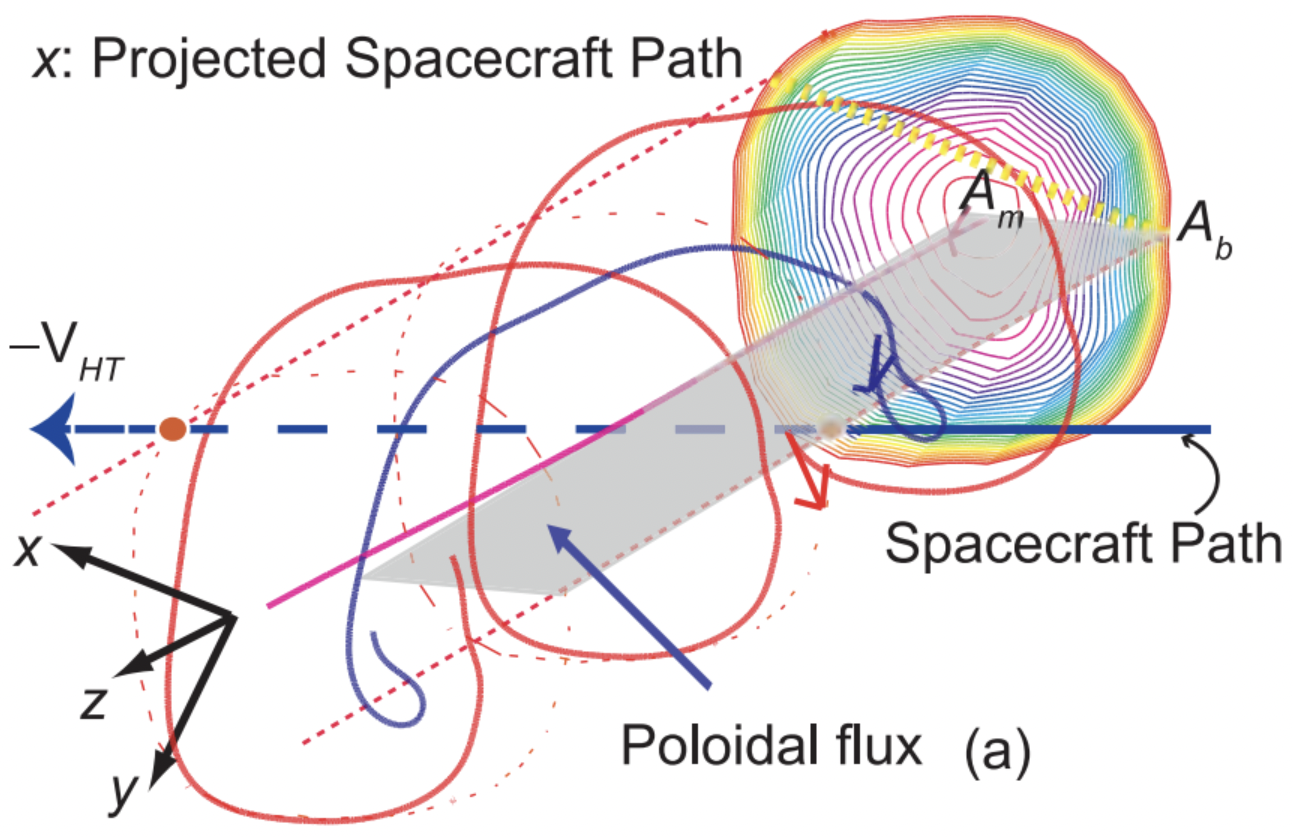
\includegraphics[width=\textwidth]{Figures/Hu2017_5a.png}
    \caption[Representation of a 2D cross-sectional view of a magnetic cloud] {View of a reconstruction for a magnetic cloud event as a spacecraft passes through it \citep{Hu:2017}. The 2D cross section and selected associated magnetic field lines (red and blue twisted lines) are shown along the flux rope axis ($z$-axis). The variables $A_m$ and $A_b$ mark the magnetic flux function $A$ at the center and boundary, respectively, of the reconstruction result. The poloidal flux and axial flux can also be obtained through the reconstruction algorithm.} %$\Phi_p = |A_m-A_b|\cdot L_{eff}$ along the effective length of the $z$-axis (shaded portion)
    \label{fig:GSreconstruction_Hu2017}
\end{figure}

\begin{figure}[ht!]
    \centering
    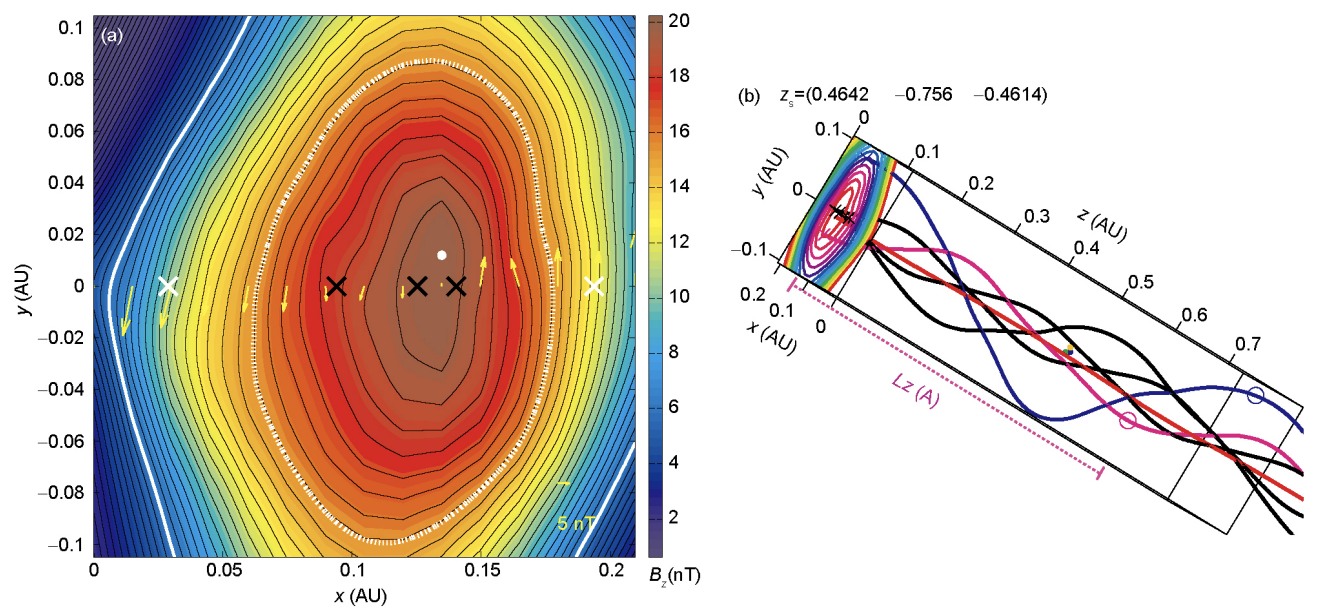
\includegraphics[width=\textwidth]{Figures/Reconstructions/Hu2015_GSreconstruction.png}
    \caption[2D reconstruction of a magnetic cloud using the GS-reconstruction algorithm]{Reconstruction of a magnetic cloud \citep{Hu:2015}: a) 2D cross section of $A(x,y)$ for a reconstructed magnetic cloud event. The black lines indicate the transverse magnetic field lines, and the color bar indicates the axial field lines $B_z$. The yellow arrows denote the transverse field lines ($B_t$) along the path of the spacecraft ($y=0$). The white contour indicates the area of the reconstruction done from spacecraft data ($A=A_b$), while the area outside the white contour is reconstructed from extrapolation. b) 3D view of a flux rope structure for the magnetic cloud event, showing the 2D cross section (A') and selected associated twisted magnetic field lines along the flux rope axis (denoted at the top). The black field lines  rooted at the foot points where the electron onsets were observed. The pink and blue circles denote the locations where the associated field lines complete a full turn around the z-axis.}
    \label{fig:GSreconstruction_Hu2015}
\end{figure}

% Determination of the cylindrical z-axes
The GS-based algorithm starts by moving a window continually through an entire data segment with variable window sizes in turn, ranging from the minimum duration of approximately 10 data points with cadence $\Delta t$, \textit{i.e.} 10$\Delta t$, to the maximum duration of 343 data points to cover a wide range of SFR duration, while taking into account limited computing resources. The maximum duration corresponds to approximately 17 minutes for the THEMIS data, and 25 minutes for the MMS data. The in situ magnetic field and plasma data from a specified window of time are first transformed into the co-moving frame, notably the de Hoffmann-Teller frame \citep{deHoffman-Teller:1950}. Through a trial-and-error process, the optimal orientation of the $z$-axis is determined. A trial $z$-axis is represented by the azimuthal and polar angles, \gls{phi} and \gls{theta}, in the GSE coordinate system. The azimuthal angle $\phi$ is the longitude of the SFR $z$-axis, which measures the angle between the GSE $X$-direction and the projection of the $z$-axis onto the $XY$-plane. The polar angle $\theta$ is the angle between the SFR $z$-axis and the $Z$-direction. The trial values for $\phi$ and $\theta$ are selected, and the transverse pressure $P_t'$ along the spacecraft path is calculated, as shown in Equation (\ref{eq:GSextended}). The plot of $P_t'$ versus $A'$ may have a turning point where $P_t'$ along the spacecraft path splits into two parts, with an extreme $A'$ value near this turning point, typically for an SFR structure. This is where the magnetic field $B_y$ component changes sign because of the field line geometry of a helical structure. To search for the double-folding of $P_t'$ versus $A'$, the line integral of $B_y$ along the spacecraft path ($y=0$) is evaluated:
\begin{equation}
    A'(x,0)=-\int_0^x\p{1-\alpha}B_y(x',0)dx'.
    \label{eq:By-integral}
\end{equation}
Figure \ref{fig:Pt-vs-A} represents such a $P_t'$ versus $A'$ plot, with two distinct portions joining near a turning point with a minimum $A'$ value. The quality of the folding (or overlapping) of the two parts of $P_t'$ versus $A'$ is evaluated by two metrics, \gls{Rdiff} (the point-wise difference residue between the two parts) and \gls{Rfit} (a residue of the fitting function $P_t'(A')$ as illustrated by the solid black curve). These metrics are used to check how well the two parts fold onto each other, provided that such a turning point exists. The threshold conditions, $R_{diff}\lesssim 0.2$ and $R_{fit}\lesssim 0.2$ for these metrics, are selected empirically to guarantee good double-folding quality \citep{Hu:2018}. The optimal orientation of the $z$-axis of the SFRs is found by going through iterations of $\phi$ and $\theta$ until the minimum residue values are found. Once the minimum residues satisfying the threshold conditions are found, the corresponding optimal $z$-axis orientation and event interval are recorded as an SFR candidate.

% \begin{figure}
%     \centering
%     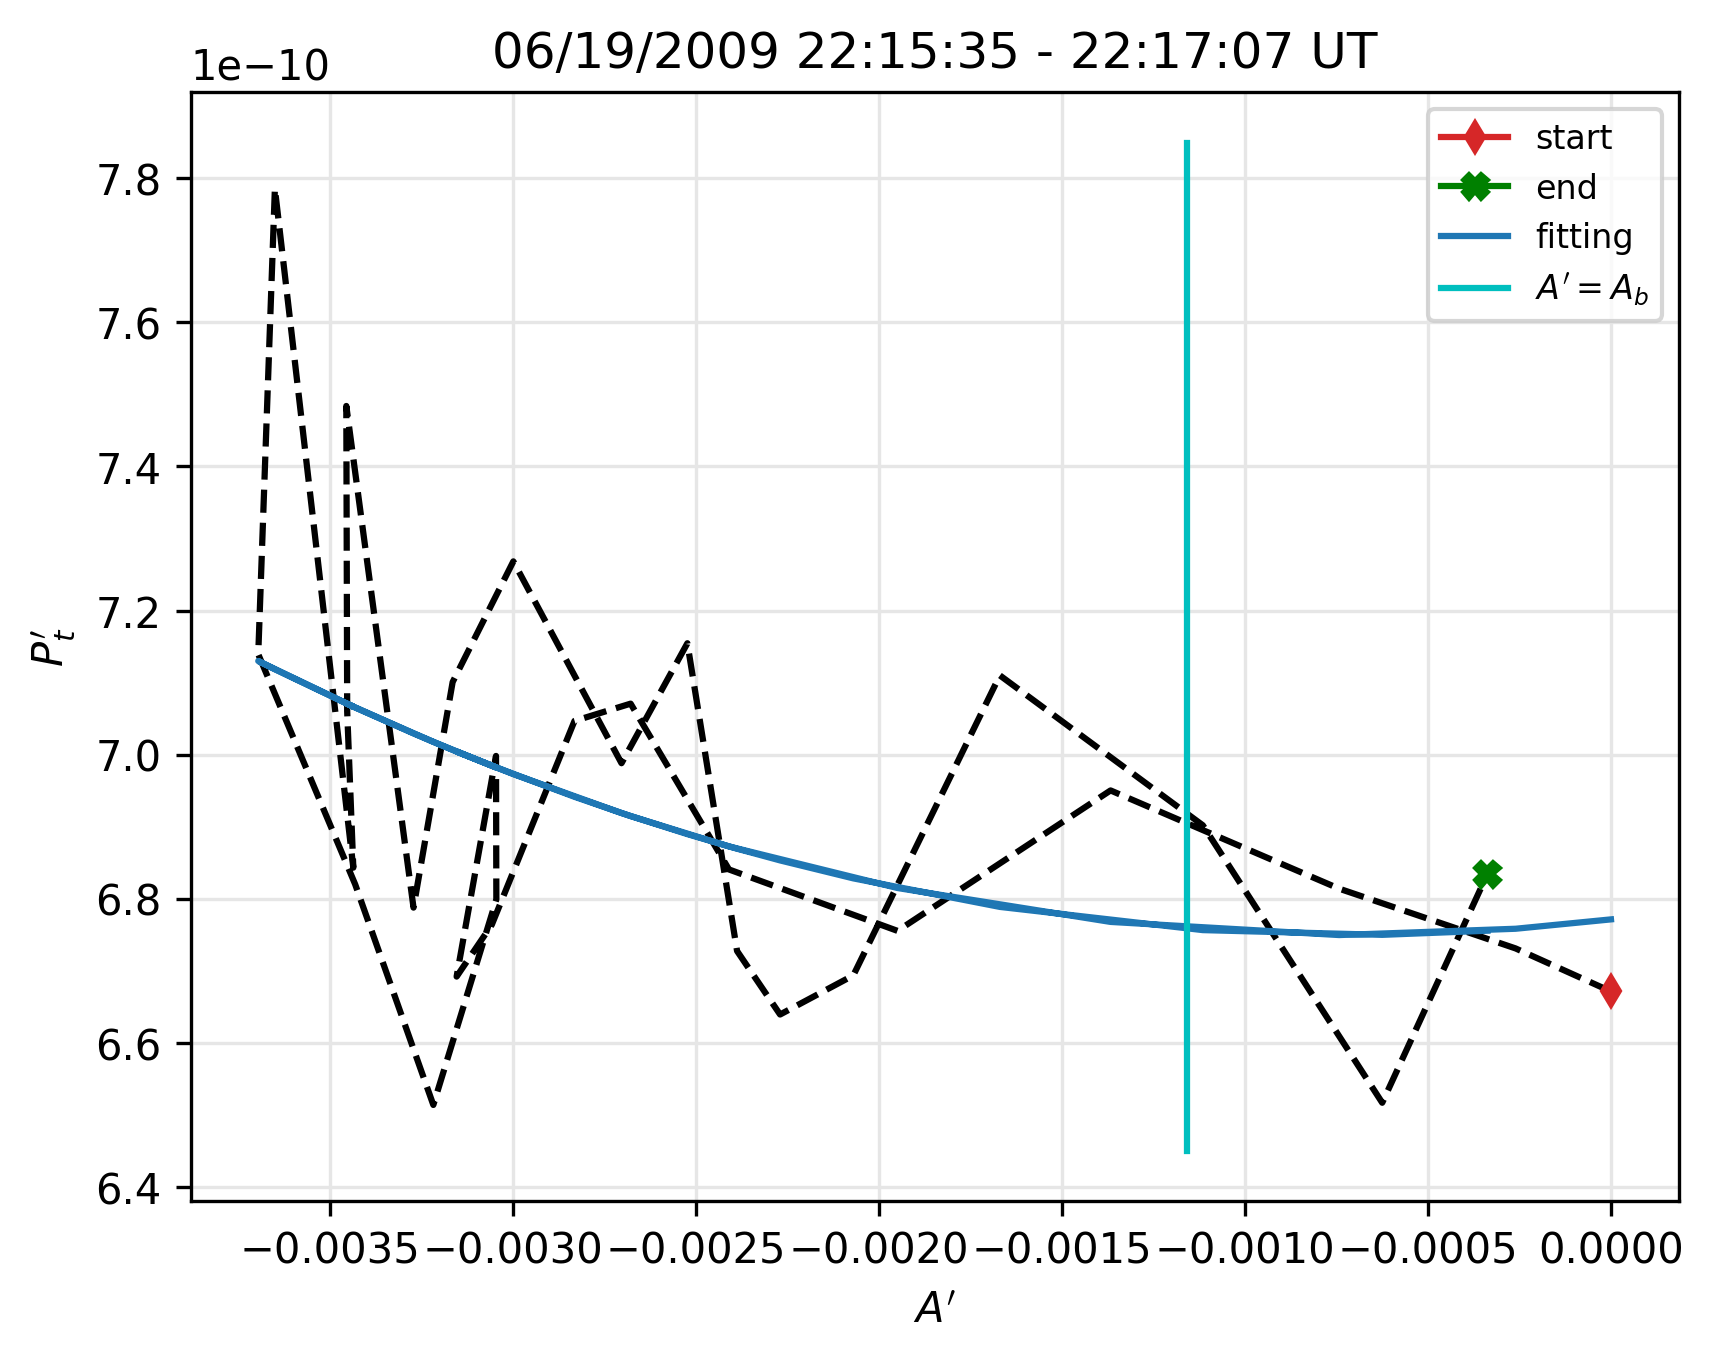
\includegraphics[width=\textwidth]{Figures/Reconstructions/PtvsA_Ab_20090619_20090621.png}
%     \caption[Double folding pattern of $P_t'$ versus $A'$ for 22:15:35-22:17:05 UT on 19 June 2009]{$P_t'(A')$ versus $A'$ plot for an SFR from 22:15:35-22:17:05 on 19 June 2009 observed by THM-C. The red and green markers indicate the starting and ending points of the SFR interval, the darker blue line indicates the fitted $P_t'(A')$ versus $A'$ function, and the lighter blue line indicates the turning point where $A'=A_b$.}
%     \label{fig:Pt-vs-A-Ab}
% \end{figure}

\begin{figure}
    \centering
    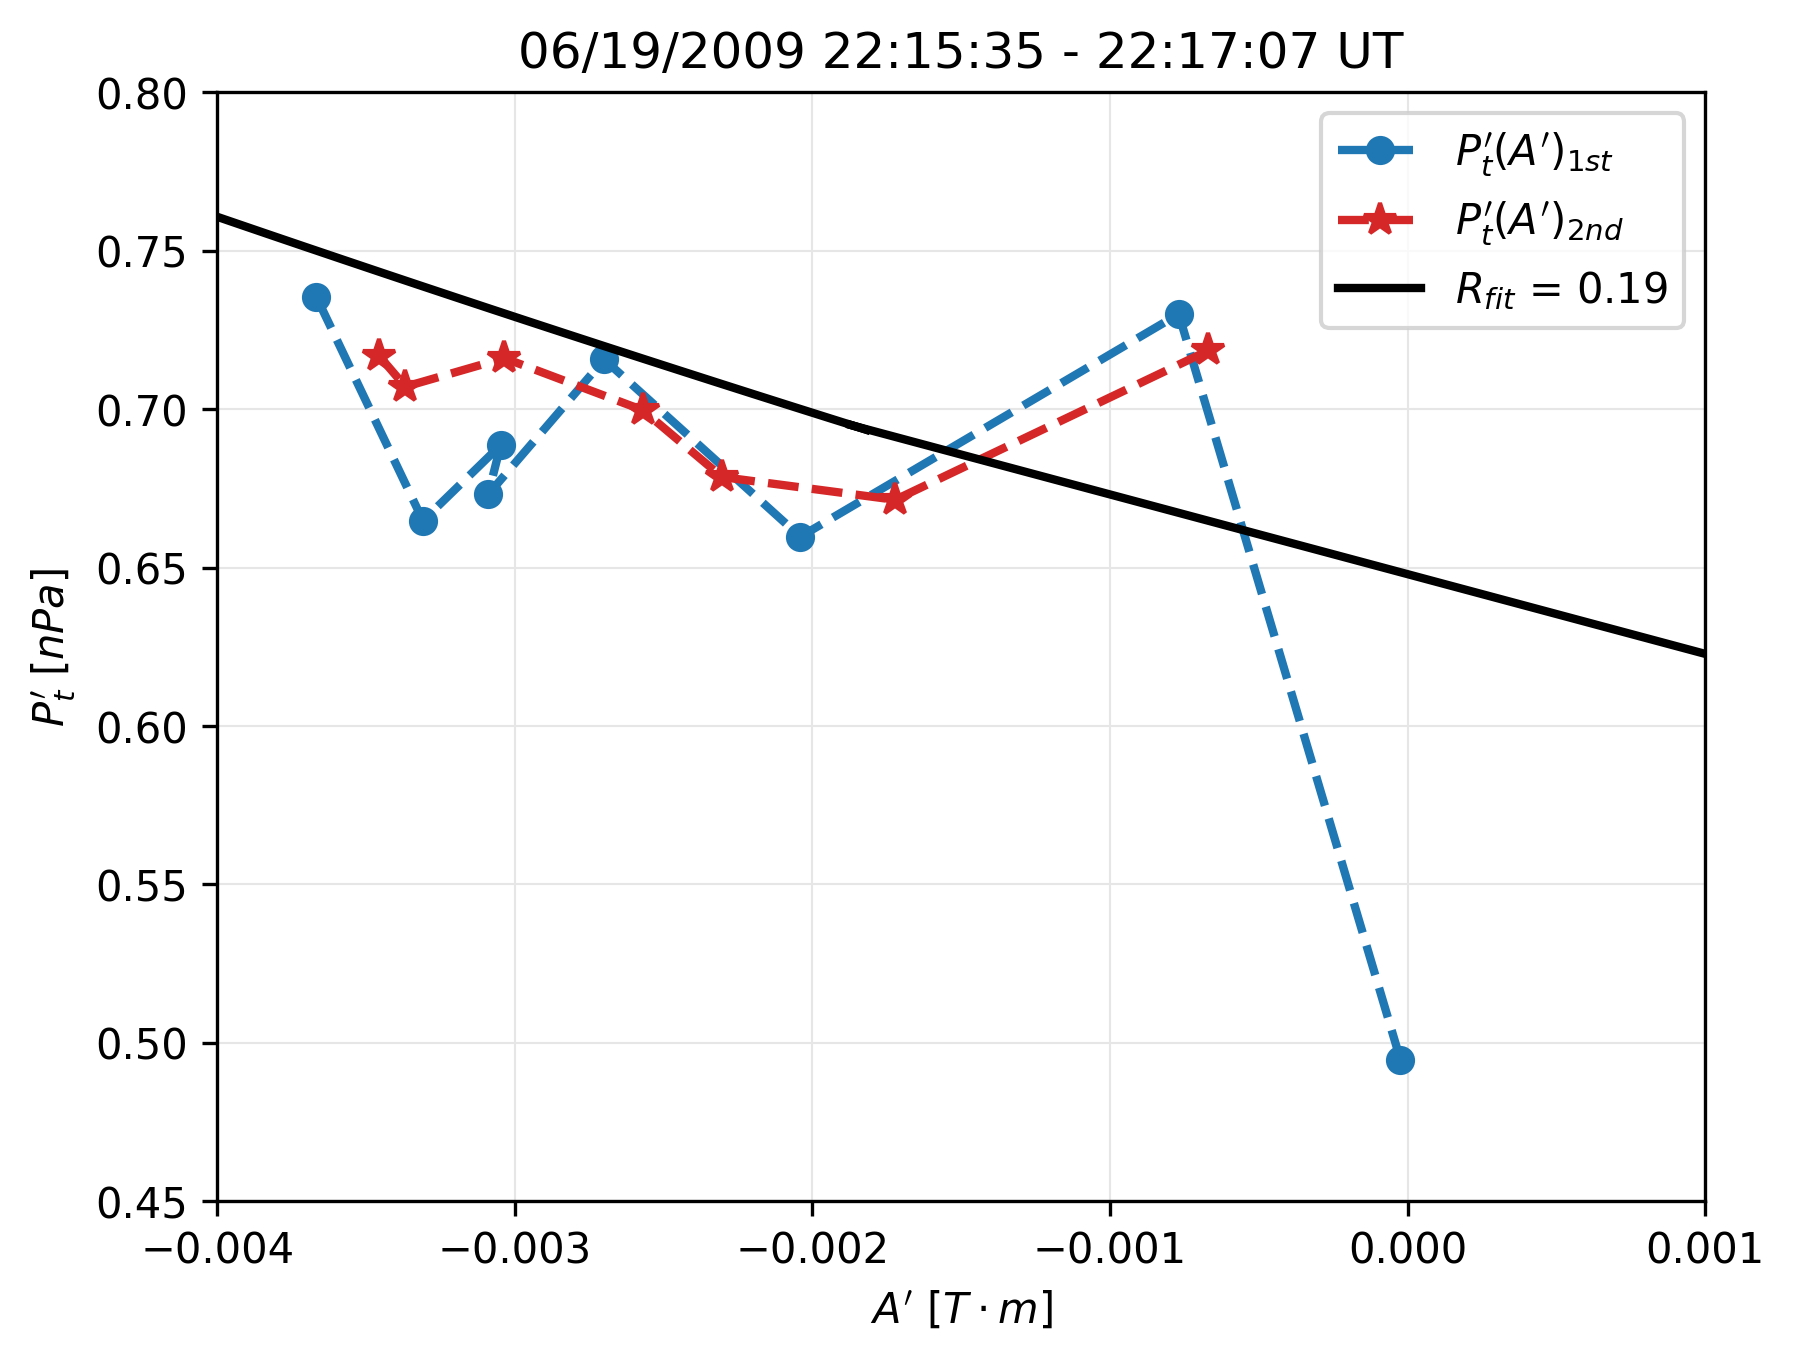
\includegraphics[width=\textwidth]{Figures/Reconstructions/PtvsA_20090619_20090621.png}
    \caption[$P_t'$ versus $A'$ plot for 22:15:35-22:17:05 UT on 19 June 2009]{The $P_t'$ versus $A'$ plot for an SFR interval from 22:15:35-22:17:05 UT on 19 June 2009 observed by THM-C. The data points are marked by the symbols, and are connected by the blue dashed line and the red dashed line, separated by the turning point at the minimum of $A'$ in this case. The two lines correspond to the first and second parts of the $P_t'(A')$ curve as denoted by the legend. The solid black curve represents a functional fitting to the data points with fitting residue $R_{fit}$.}
    \label{fig:Pt-vs-A}
\end{figure}

% The data are then used to calculate the transverse pressure $P_t'(A')$ as a function of the scalar flux function, $A'$. If the $P_t'$ versus $A'$ is double folded through a flux rope interval, then two metrics, $R_{diff}$ (the point-wise difference between the two folds) and $R_{fit}$ (a fitting residue of $P_t'(A')$), are used to check the double-folding quality and the shape of $P_t'(A')$. The threshold values for these metrics are selected empirically to guarantee good flux rope quality \citep{Hu:2018}, and if the thresholds are met, the event is recorded as an event candidate. If the thresholds are not met, the $z$-axis will go through its next iteration until the thresholds are met.

After the initial detection of SFR candidates, the list of initial candidates is refined. The records are further classified based on the Wal\'en test slope \gls{walen}, which is the slope of the linear regression between $\mathbf{V_{sw}} - \mathbf{V_{HT}}$ and $\mathbf{V_A}$. Records with $|w|\leq0.3$ are quasi-static SFRs and thus saved directly. Records with $|w|>0.3$, except for when the correlation coefficient $r$ between the aforementioned two velocities ($\mathbf{V_{sw}} - \mathbf{V_{HT}}$ and $\mathbf{V_A}$) is $|r|\geq 0.8$ and $\langle M_A\rangle \leq 0.9$, are removed. These conditions ensure that the remaining plasma flow is aligned with the local magnetic field, and also to avoid a singularity in Equation (\ref{eq:GSextended}) at $\alpha=1$. Events with $\alpha>1$ are rare, but they are also removed, so that the events remaining are sub-Alfv\'enic. The algorithm also removes events from the initial candidate list if the candidates have a turning point within $5\Delta t$ (turn time) of the turning point of another candidate with a smaller $R_{diff}$, as these could be the same overlapping structures. Table \ref{tab:thresholds} lays out the threshold conditions as utilized in the post-processing of the GS-based detection event list \citep{Chen:2020, Chen:2021, Chen:2022}.
\begin{table}[h!]
\centering
\caption[Threshold conditions for GS algorithm]{Table of threshold conditions for GS reconstruction-based algorithm. $R_{diff}$ and $R_{fit}$ are residues which ensure good double-folding quality in the $P_t'(A')$ vs. $A'$ curve..} %Events meeting the following criteria are kept.} %Duration is $10*dt\sim 343*dt$ where $dt\sim 3$ seconds.
\begin{tabular}{ccccccc}
\toprule
    Duration  & $R_{diff}$ & $R_{fit}$ & Turn time & Wal\'en test slope & $|r|$ & $\langle M_A\rangle$ \\ 
    \hline
    %$\sim$ 30-1029 & $<0.2$ & $<0.2$ & 5$dt$ & $\leq 1$ &  &  \\
    10$\Delta t$-342$\Delta t$ & $<0.2$ & $<0.2$ & 5$\Delta t$ & $|k|\leq 0.3$ & & \\
    10$\Delta t$-342$\Delta t$ & $<0.2$ & $<0.2$ & 5$\Delta t$ & $|k|> 0.3$ & $\geq 0.8$ & $\leq 0.9$ \\
\bottomrule %30-1029 (s)
\end{tabular}
\label{tab:thresholds}
\end{table}

%Solar wind
%k <= 0.3:  1752
%k > 0.3; r>|0.8|, <M_A> <0.9:  107

% Magnetosheath
%k <= 0.3:  2310
%k > 0.3; r>|0.8|, <M_A> <0.9:  70

The duration of the search windows does not exceed 343$\Delta t$ ($\sim25.733$ minutes for MMS and $\sim24.553$ minutes for THEMIS) due to computational time constraints. The detection algorithm was performed for some time periods with search window size up to 388 points in duration; however, the search yielded very few (generally less than 3) additional event counts after the post-processing steps. This was due to the step of making sure there is no overlap between SFR candidates, which prioritizes smaller duration candidates. Therefore, with the search algorithm taking a significant amount of time to run for longer search windows and yielding very few results, it was decided to stop the search at the maximum window size of $343\Delta t$.

The PyGS software \citep{Zheng:2018, Hu:2018, Chen:2022, Sonnerup:1996, Hau:1999, HuSonnerup:2002} was used to reconstruct the 2D cross-sections and search for the folding patterns in the $P_t'$ versus $A'$ plot. Some modifications to the post-processing portion of the search algorithm were made in order to adhere to the magnetosheath environment. In one step of the post-processing algorithm, SFR candidates containing shocks (and other discontinuities) identified by various spacecraft (see PyGS documentation at \url{https://github.com/PyGSDR/PyGS}) are removed. Because the behavior of plasma in the magnetosheath is highly turbulent, removing SFR candidates with discontinuities would not be appropriate.
%Another adjustment in post-processing candidates was the 
%Other user-input values, such as the turn-time tolerance and thresholds for $R_{diff}$ and $R_{fit}$ were adjusted, and do not follow the published PyGS package values.

\section{2D reconstructions of cross-sections}
Figures \ref{fig:reconstruction-Nov2019} and \ref{fig:reconstruction-June2009} are examples of the reconstruction of 2D cross-sections of selected flux rope events, both in the magnetosheath. The black lines indicate the transverse magnetic field lines, and the color background indicates the axial field $B_z$ with the strength denoted by the color bar. The flux rope structure is confirmed by the closed field lines region and unipolar $B_z$. The white dot indicates the maximum $B_z$. The white arrows denote the transverse magnetic field lines ($\Bvec_t$) along the path of the spacecraft ($y=0$), and the green arrows along this path denote the remaining flow velocity. The white contour encloses the area of the reconstruction done from spacecraft data, while the area outside the white contour is reconstructed from extrapolation.

\begin{figure}[ht!]
    \centering
    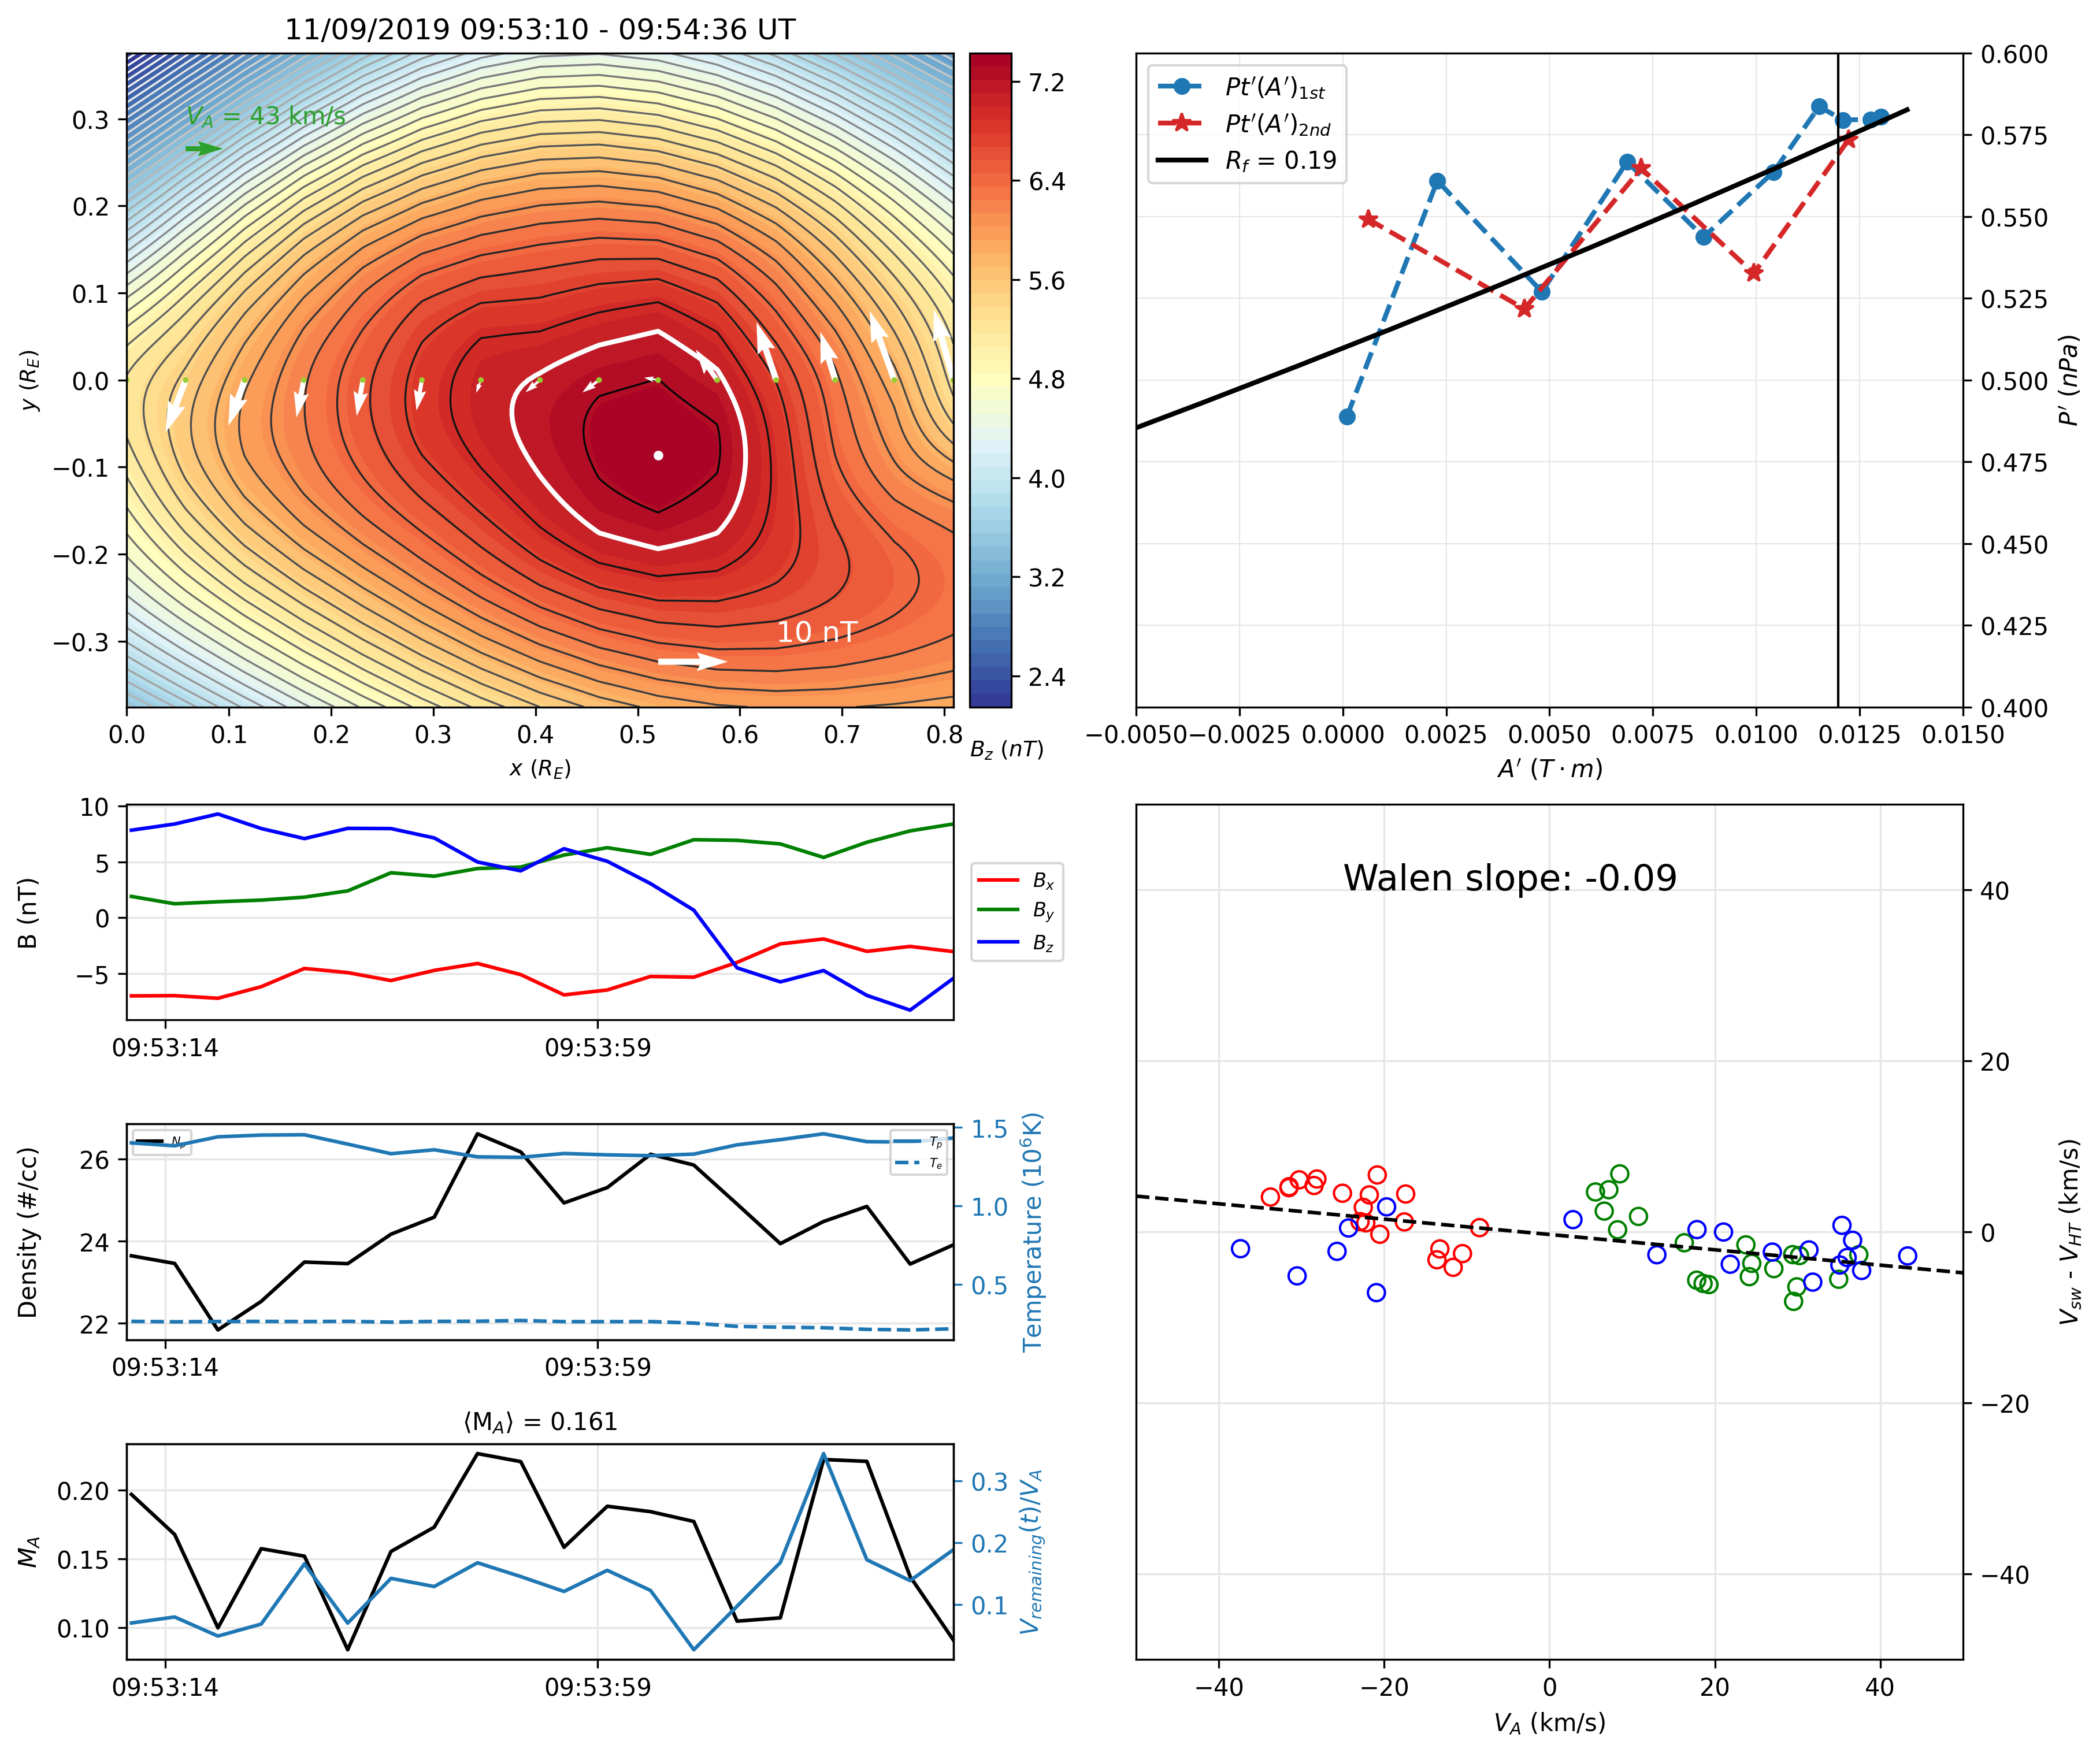
\includegraphics[width=\textwidth]{Figures/Reconstructions/timeseries_walenTest_20191109_20191110.png}
    \caption[GS-based event reconstruction for 9 November 2019]{GS-based reconstruction of an event 9:53:10-9:54:36 UT on 9 November 2019 in the magnetosheath. Top left: 2D cross-section, with $\hat{x}_{GSE}=[0.890, 0.268, 0.369]$, $\hat{y}_{GSE}=[0.142, 0.605, -0.784]$, $\hat{z}_{GSE}=[-0.433, 0.750, 0.500]$. Bottom left: Associated time series data for MMS-1 in the magnetosheath during this period. Top right: $P_t'(A')$ vs. $A'$ curve for this event. Bottom right: Wal\'en relation for this event.}
    \label{fig:reconstruction-Nov2019}
\end{figure}

\begin{figure}[ht!]
    \centering
    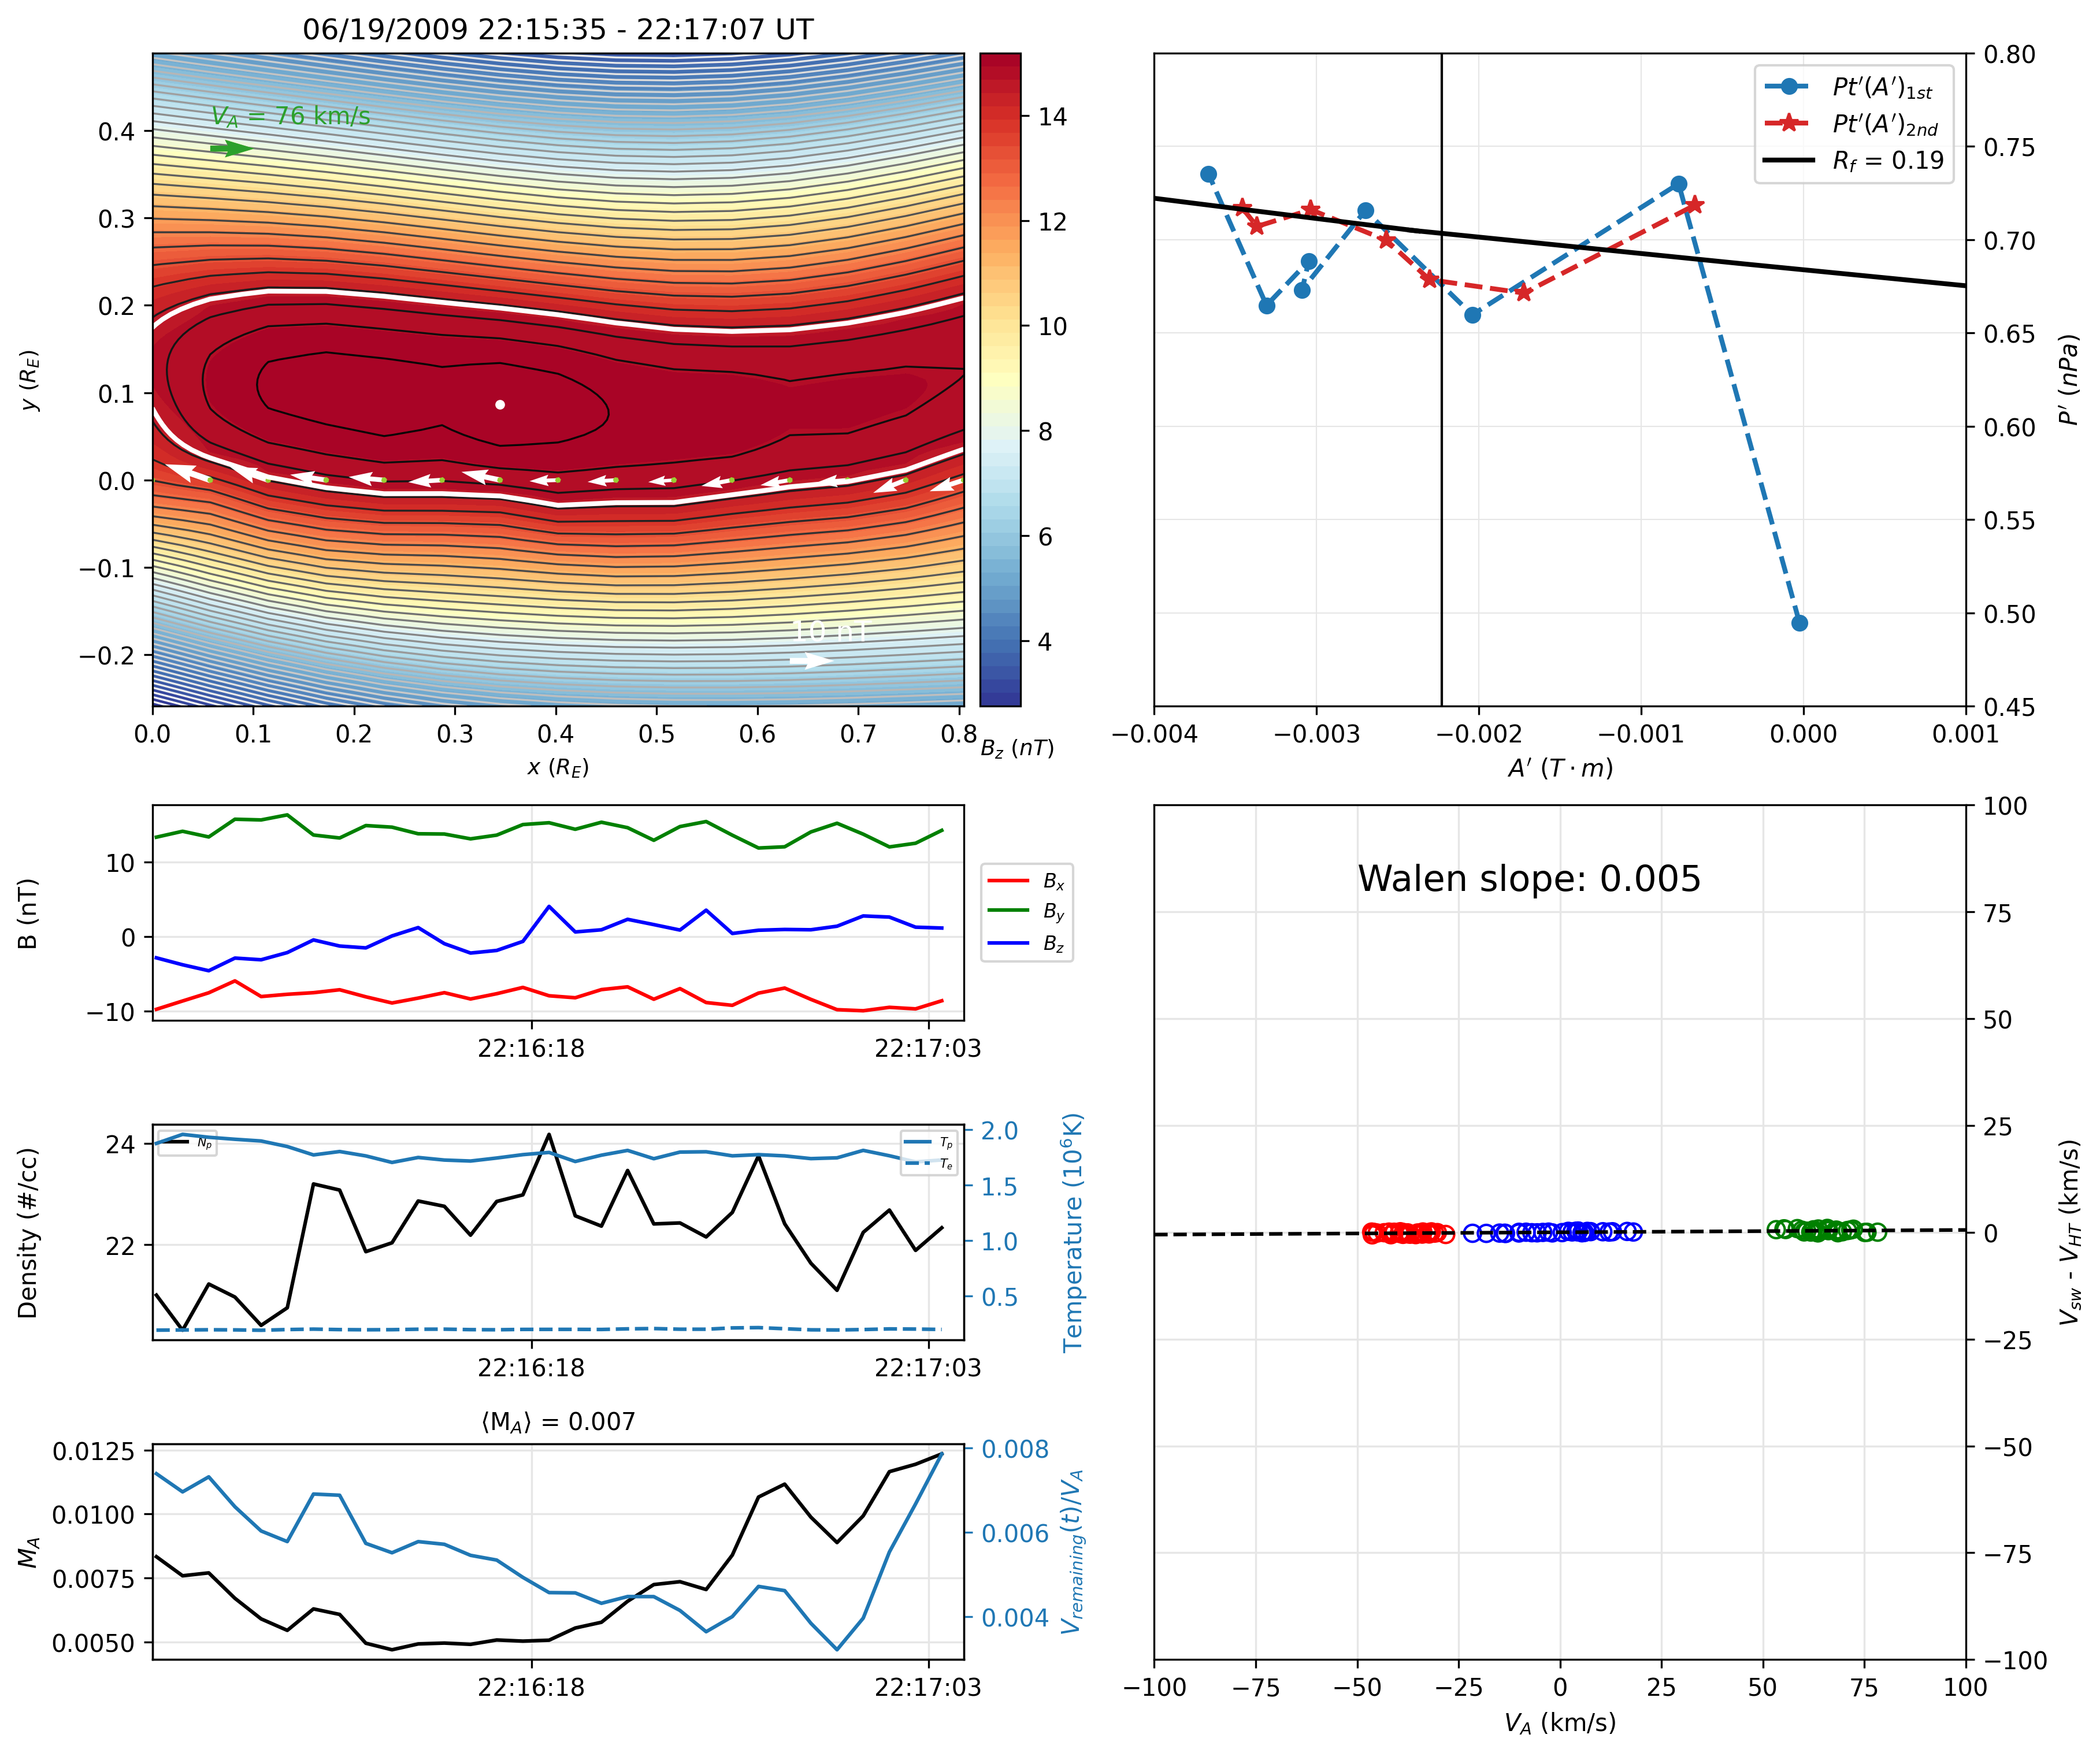
\includegraphics[width=\textwidth]{Figures/Reconstructions/timeseries_walenTest_20090619_20090621.png}
    \caption[GS-based event reconstruction for 19 June 2009]{GS-based reconstruction of an event from 22:15:35-22:17:07 UT on 19 June 2009 in the magnetosheath. Top left: 2D cross-section, with $\hat{x}_{GSE}=[0.761, -0.103, 0.640]$, $\hat{y}_{GSE}=[0.628, 0.365, -0.688]$, $\hat{z}_{GSE}=[-0.163,0.925,0.342]$. Bottom left: Associated time series data for THM-C in the magnetosheath during this period. Top right: $P_t'(A')$ vs. $A'$ curve for this event. Bottom right: Wal\'en relation for this event.}
    \label{fig:reconstruction-June2009}
\end{figure}

The event in Figure \ref{fig:reconstruction-Nov2019} has a Wal\'en slope of -0.09, and the event in Figure \ref{fig:reconstruction-June2009} has a Wal\'en test slope of 0.002. This indicates that the structures are static, where the remaining flow vectors (green) along the spacecraft path in the cross-section have little alignment with the transverse magnetic field line vectors (white arrows). The closed, transverse field lines, and the $B_t$ vectors along the spacecraft path show that the reconstruction in Figure \ref{fig:reconstruction-Nov2019} is a right-handed event, while the structure in Figure \ref{fig:reconstruction-June2009} is a left-handed flux rope. The maximum $B_z$ of the structure in Figure \ref{fig:reconstruction-Nov2019} is 11.85 nT, and that of the structure in Figure \ref{fig:reconstruction-June2009} is 18.21 nT. Figure \ref{fig:reconstruction-Nov2017-quasistatic} shows the reconstruction of a left-handed, quasi-static event in the magnetosheath. It has a much larger scale size ($\sim5 R_E$) than those in the magnetosheath ($\lesssim1 R_E$). The Wal\'en test slope of this event is 0.399, which meets the $|w| > 0.3$ threshold. It can be seen that the structure has a considerable remaining flow, as indicated by the size of the green arrows.
\begin{figure}
    \centering
    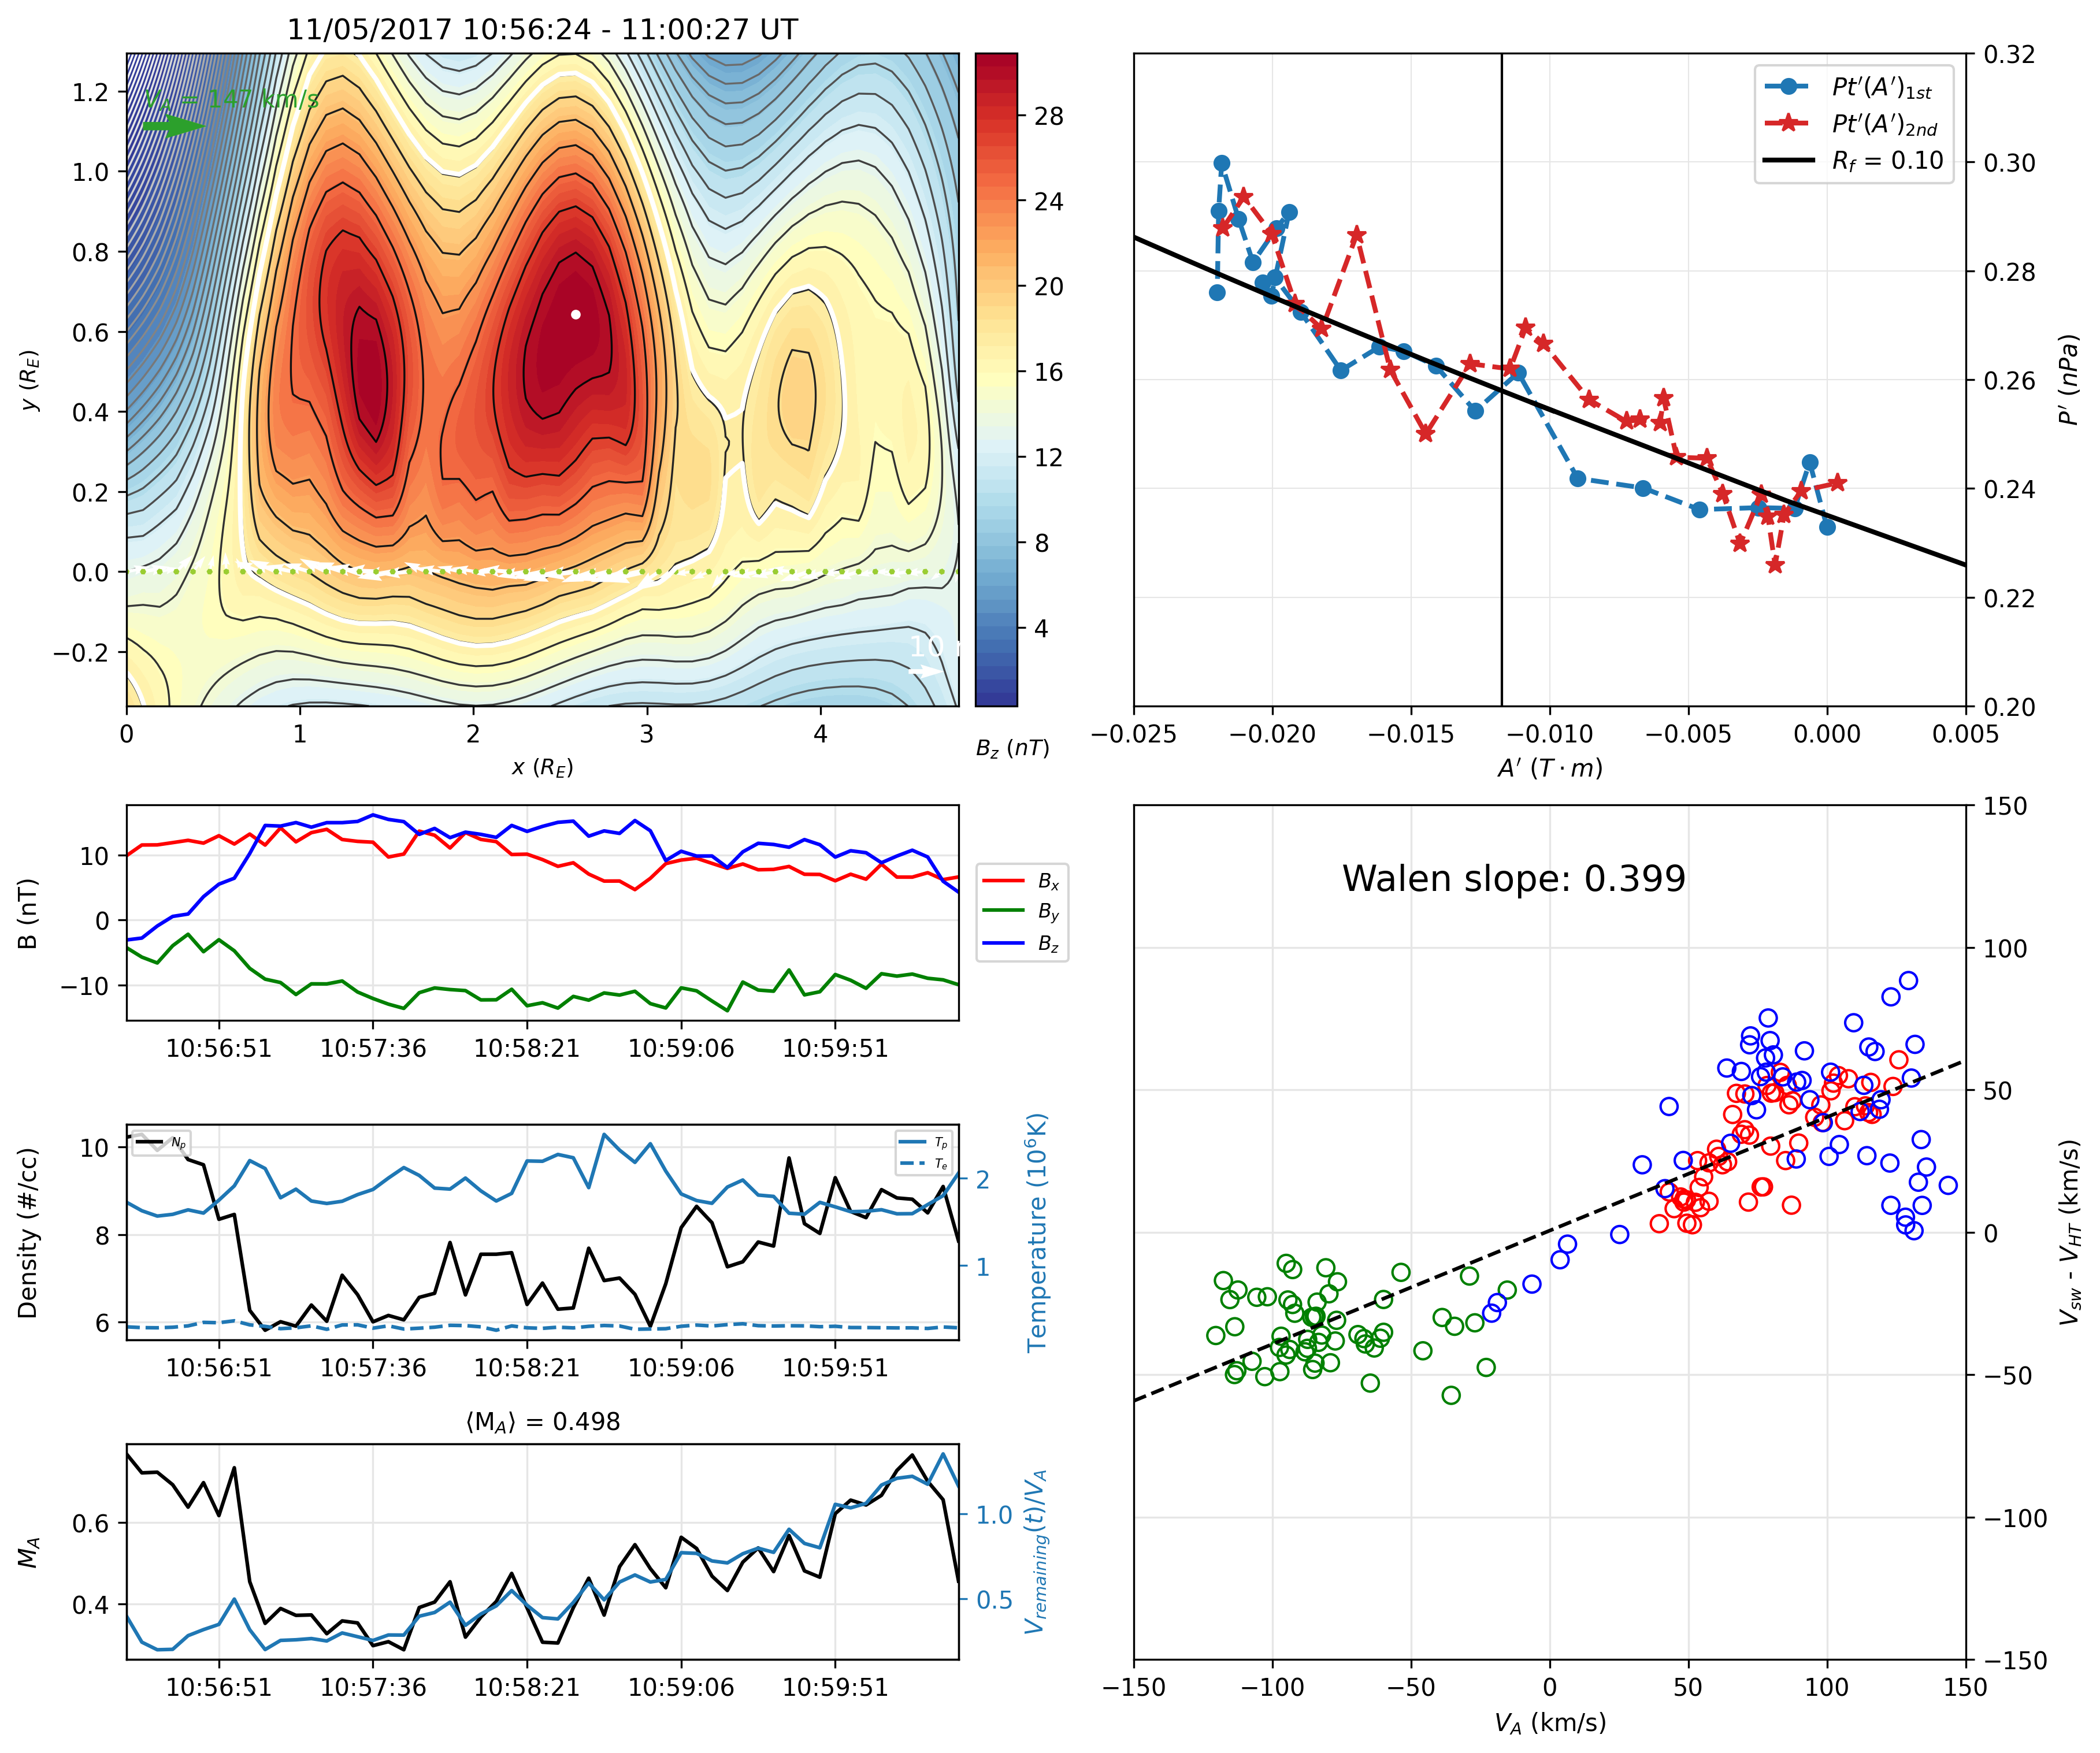
\includegraphics[width=\textwidth]{Figures/Reconstructions/timeseries_walenTest_20171105_20171106.png}
    \caption[GS-based event reconstruction for 15 November 2017]{GS-based reconstruction of an event on 10:56:24-11:00:27 UT on 5 November 2017 in the magnetosheath. Top left: 2D cross-section, with $\hat{x}_{GSE}=[0.409, -0.029, -0.912]$, $\hat{y}_{GSE}=[0.561, 0.796, 0.226]$, and $\hat{z}_{GSE}=[0.720, -0.604, 0.342]$. Bottom left: Associated time series data for MMS-1 in the magnetosheath during this period. Top right: $P_t'(A')$ vs. $A'$ curve for this event. Bottom right: linear regression of the remaining flow $V_{rem}$ versus the Alfv\'en velocity $V_A$, with Wal\'en slope for this event being 0.399.} % B_z = 41.19 nT
    \label{fig:reconstruction-Nov2017-quasistatic}
\end{figure}

\section{Analysis results}
Table \ref{tab:regions-GS-summary} summarizes the events identified in the solar wind and magnetosheath across the identified time periods: 19 in the solar wind and 19 in the magnetosheath simultaneously from two spacecraft, and an additional 58 periods in the solar wind and 111 in the magnetosheath (including those from the refined \cite{ToyEdens:2024} list). The occurrence rate for events in the solar wind from the GS-based is about 5.1 events/hour and for the magnetosheath the corresponding rate is about 7.3 events/hour. SFRs are observed approximately in 43\% and 44\% of the total observation periods in the solar wind and magnetosheath, respectively. Properties of the magnetic structures are recorded during the identification process. The average duration of the events identified with the GS-based method is 5.03 minutes for the solar wind and 3.57 minutes for the magnetosheath. The average magnetic field for the identified events is 4.8 nT in the solar wind and 21.6 nT in the magnetosheath.

\begin{table}
    \centering
    \caption{Summary table for identified events in the solar wind and magnetosheath via the GS-based reconstruction identification algorithm.}
    \begin{tabular}{rccc}
\hline
                        & Observation        & Events & Event rate \\
                        & period [hrs]       &        & [\#/hour]  \\
\hline
\textit{Solar wind}     & 676 hours          &  3476  & 5.1 \\
\textit{Magnetosheath}  & 1051 hours         &  7689  & 7.3 \\
\hline
\end{tabular}
    \label{tab:regions-GS-summary}
\end{table}

Table \ref{tab:stats-GS} summarizes the statistical values for the events identified with the GS-based analysis. In the solar wind, there are a large number of events with an average magnetic field of less than 10 nT, whereas in the magnetosheath there are relatively much fewer events with $\langle B\rangle < 10$ nT. The median magnetic field magnitude in the solar wind is 4.3 nT, and 17.9 nT in the magnetosheath. The mean $\langle B\rangle$ in the magnetosheath is $\sim$20 nT for all of the events identified. In the solar wind, this number is much smaller around 4.9 nT. As shown in Table \ref{tab:stats-GS}, the duration of the events has similar ranges for the two regions. However, for the scale sizes of the GS events in the magnetosheath, they range from 251.7 km to 6$\times 10^5$ km, with a median and mean of 1.6$\times 10^4$ km, $\sim$2.5$R_E$ and 3.8$\times 10^4$ km, $\sim$6.0 $R_E$, respectively. In the solar wind, the corresponding values are from 1296.1 km to 8.6$\times 10^5$ km, and a median (mean) of 2.9$\times 10^4$ (9.1$\times 10^4$) km, $\sim$4.6 (14) $R_E$.

\begin{table}
    \centering
    \caption[Statistical values for the physical quantities of structures identified with GS-based analysis analysis]{Statistical values for the physical quantities of the structures identified with the GS-based analysis. Top: magnetosheath; bottom: solar wind.}
    \begin{tabular}{lccccc}
\hline
                       & Minimum & Maximum & Mean & Median & Std. Dev. \\
\hline
Duration [min]         &     0.4 &      25.7 &      3.6 &     1.5 &       4.8 \\
Velocity [km/s]        &    12.0 &     547.8 &    211.4 &   203.5 &      81.1 \\
Temperature [10$^6$ K] &     0.6 &      29.2 &      3.2 &     2.3 &       2.5 \\
$<B>$ [nT]             &     2.0 &      95.2 &     21.6 &    17.9 &      12.7 \\
Scale size [km]        &   251.7 & 6.0$\times 10^5$ & 3.8$\times 10^4$ & 1.6$\times 10^5$ &   5.6$\times 10^4$ \\

\hline \hline

Duration [min]          &     0.4 &      25.7 &      5.0 &     1.6 &       6.6 \\
Velocity [km/s]         &   255.8 &     666.0 &    365.7 &   340.2 &      87.2 \\
Temperature [10$^6$ K]  &     0.1 &      15.2 &      3.2 &     3.1 &       3.5 \\
$<B>$ [nT]              &     0.7 &      19.9 &      4.8 &     4.3 &       2.5 \\
Scale size [km]         &  1296.1 & 8.6$\times 10^5$ & 9.1$\times 10^4$ & 2.9$\times 10^4$ &  1.3$\times 10^5$ \\
\hline
\end{tabular}
    \label{tab:stats-GS}
\end{table}

% histograms of GS parameters: alpha, z-axis, flux
The GS-based method can generate a set of unique physical parameters \citep{Hu:2017} as summarized in Table \ref{tab:stats-GS-only}. They include the approximate axial magnetic flux, \gls{axial flux}, a product of $\langle B_z\rangle$ and $\pi(\textnormal{scale size}/2)^2$, the poloidal magnetic flux per meter, $|A_m| = \textnormal{max}(|A|)$, and the approximate helicity density per meter $\Phi_z|A_m|$ \citep{Hu:2014}. In addition, the statistics for the proportionality parameter $\alpha$ are also presented. It generally indicates a modest level of Alfv\'enicity in both the solar wind and in the magnetosheath. The last two rows in the top and bottom blocks of Table \ref{tab:stats-GS-only} provide a proxy to the estimated magnetic helicity per unit volume. No clear differences are seen in the distributions and statistics for $\Phi_z$ and \gls{poloidal flux} between the two regions.
\begin{table}[ht!]
    \caption[Statistical values for the physical quantities of SFR structures identified solely via the GS-based method]{Statistical values for the physical quantities characterizing the SFR structures identified solely via the GS-based method in the two regions. Top: magnetosheath; bottom: solar wind.}
    \centering
    \begin{tabular}{llcccc}
\hline
 &  Criteria & Minimum & Maximum & Mean & Median \\
\hline
$\Phi_z$ [Tm$^2$]                    &              & 403.8               & 4.8$\times 10^{9}$  & 4.9$\times 10^{7}$ & 2.1$\times 10^{6}$ \\
\multirow[t]{3}{*}{$|A_m|$ [Tm]}     &              & 3.1$\times 10^{-5}$ & 3.6                 & 0.04               & 9.2$\times 10^{-3}$ \\    
Helicity Density [T$^2$m$^3$]        &              & 0.01                & 1.7$\times 10^{10}$ & 1.4$\times 10^{7}$ & 1.9$\times 10^{4}$ \\
\multirow[t]{2}{*}{$\alpha=<M_A>^2$} & $|w|\leq0.3$ & 1.3$\times 10^{-6}$ & 0.99                & 0.14               & 0.06 \\
                                     & $|w|>0.3$    & 0.09                & 0.81                & 0.37               & 0.32 \\                        
$\langle |A| \cdot B_z \rangle$  [T$^2$ m]  & & 4.0$\times 10^{-14}$ & 3.0$\times 10^{-8}$ & 3.1$\times 10^{-10}$ & 4.7$\times 10^{-11}$ \\
max($|A| \cdot B_z$) [T$^2$ m]              & & 7.4$\times 10^{-14}$ & 1.0$\times 10^{-7}$ & 7.7$\times 10^{-10}$ & 1.1$\times 10^{-10}$ \\
\hline \hline
$\Phi_z$ [Tm$^2$]                    &              & 375.5               &  4.9$\times 10^{9}$ & 8.7$\times 10^{7}$ & 2.1$\times 10^{6}$ \\   
\multirow[t]{3}{*}{$|A_m|$ [Tm]}     &              & 2.3$\times 10^{-5}$ & 1.6                 & 0.03               & 4.0$\times 10^{-3}$\\
Helicity Density [T$^2$m$^3$]        &              & 0.01                & 2.0$\times 10^{9}$  & 1.9$\times 10^{7}$ & 6.9$\times 10^{3}$ \\
\multirow[t]{2}{*}{$\alpha=<M_A>^2$} & $|w|\leq0.3$ & 1.4$\times 10^{-6}$ & 0.81                & 0.06               & 7.6$\times 10^{-3}$ \\
                                     & $|w|>0.3$    & 0.09                & 0.81                & 0.34               & 0.30 \\
$\langle |A| \cdot B_z \rangle$ [T$^2$ m]  & & 1.3$\times 10^{-15}$ & 5.4$\times 10^{-9}$ & 8.8$\times 10^{-11}$ & 5.3$\times 10^{-12}$ \\
max($|A| \cdot B_z$) [T$^2$ m]             & & 1.9$\times 10^{-15}$ & 1.0$\times 10^{-8}$ & 1.8$\times 10^{-10}$ & 1.1$\times 10^{-11}$ \\
\hline
\end{tabular}

    \label{tab:stats-GS-only}
\end{table}


Figure \ref{fig:histogram-flux} displays the distributions of the approximation to the axial flux and poloidal flux (per unit length) for events identified via the GS-based automated algorithm. Both distributions follow approximate and similar power laws in both regions. The magnetosheath exhibits events corresponding to the maximum magnitude of $|A_m|$ values larger than that in the solar wind, but these counts are few. The mean $|A_m|$ in the solar wind (0.031 Tm) is only slightly lower than that in the magnetosheath (0.035 Tm), and all corresponding statistical values are of the same orders of magnitude. For completeness, Figure \ref{fig:histogram-helicitydensity} shows the distribution of the approximation to the helicity density per unit length. The sample size needs to be enlarged to discern any differences between the two distributions. The statistical values for the helicity density per meter for the events in the magnetosheath are generally of the same orders of magnitude as those in the solar wind, except for the maximum and that the median for the magnetosheath is $\sim$2.5 times larger than that of the solar wind. On the other hand, the statistical values for the helicity density per unit volume in the magnetosheath are typically larger than those in the solar wind by one order of magnitude. This is likely an indication of compression of the SFR structures downstream of the bow shock.
\begin{figure}
    \centering
    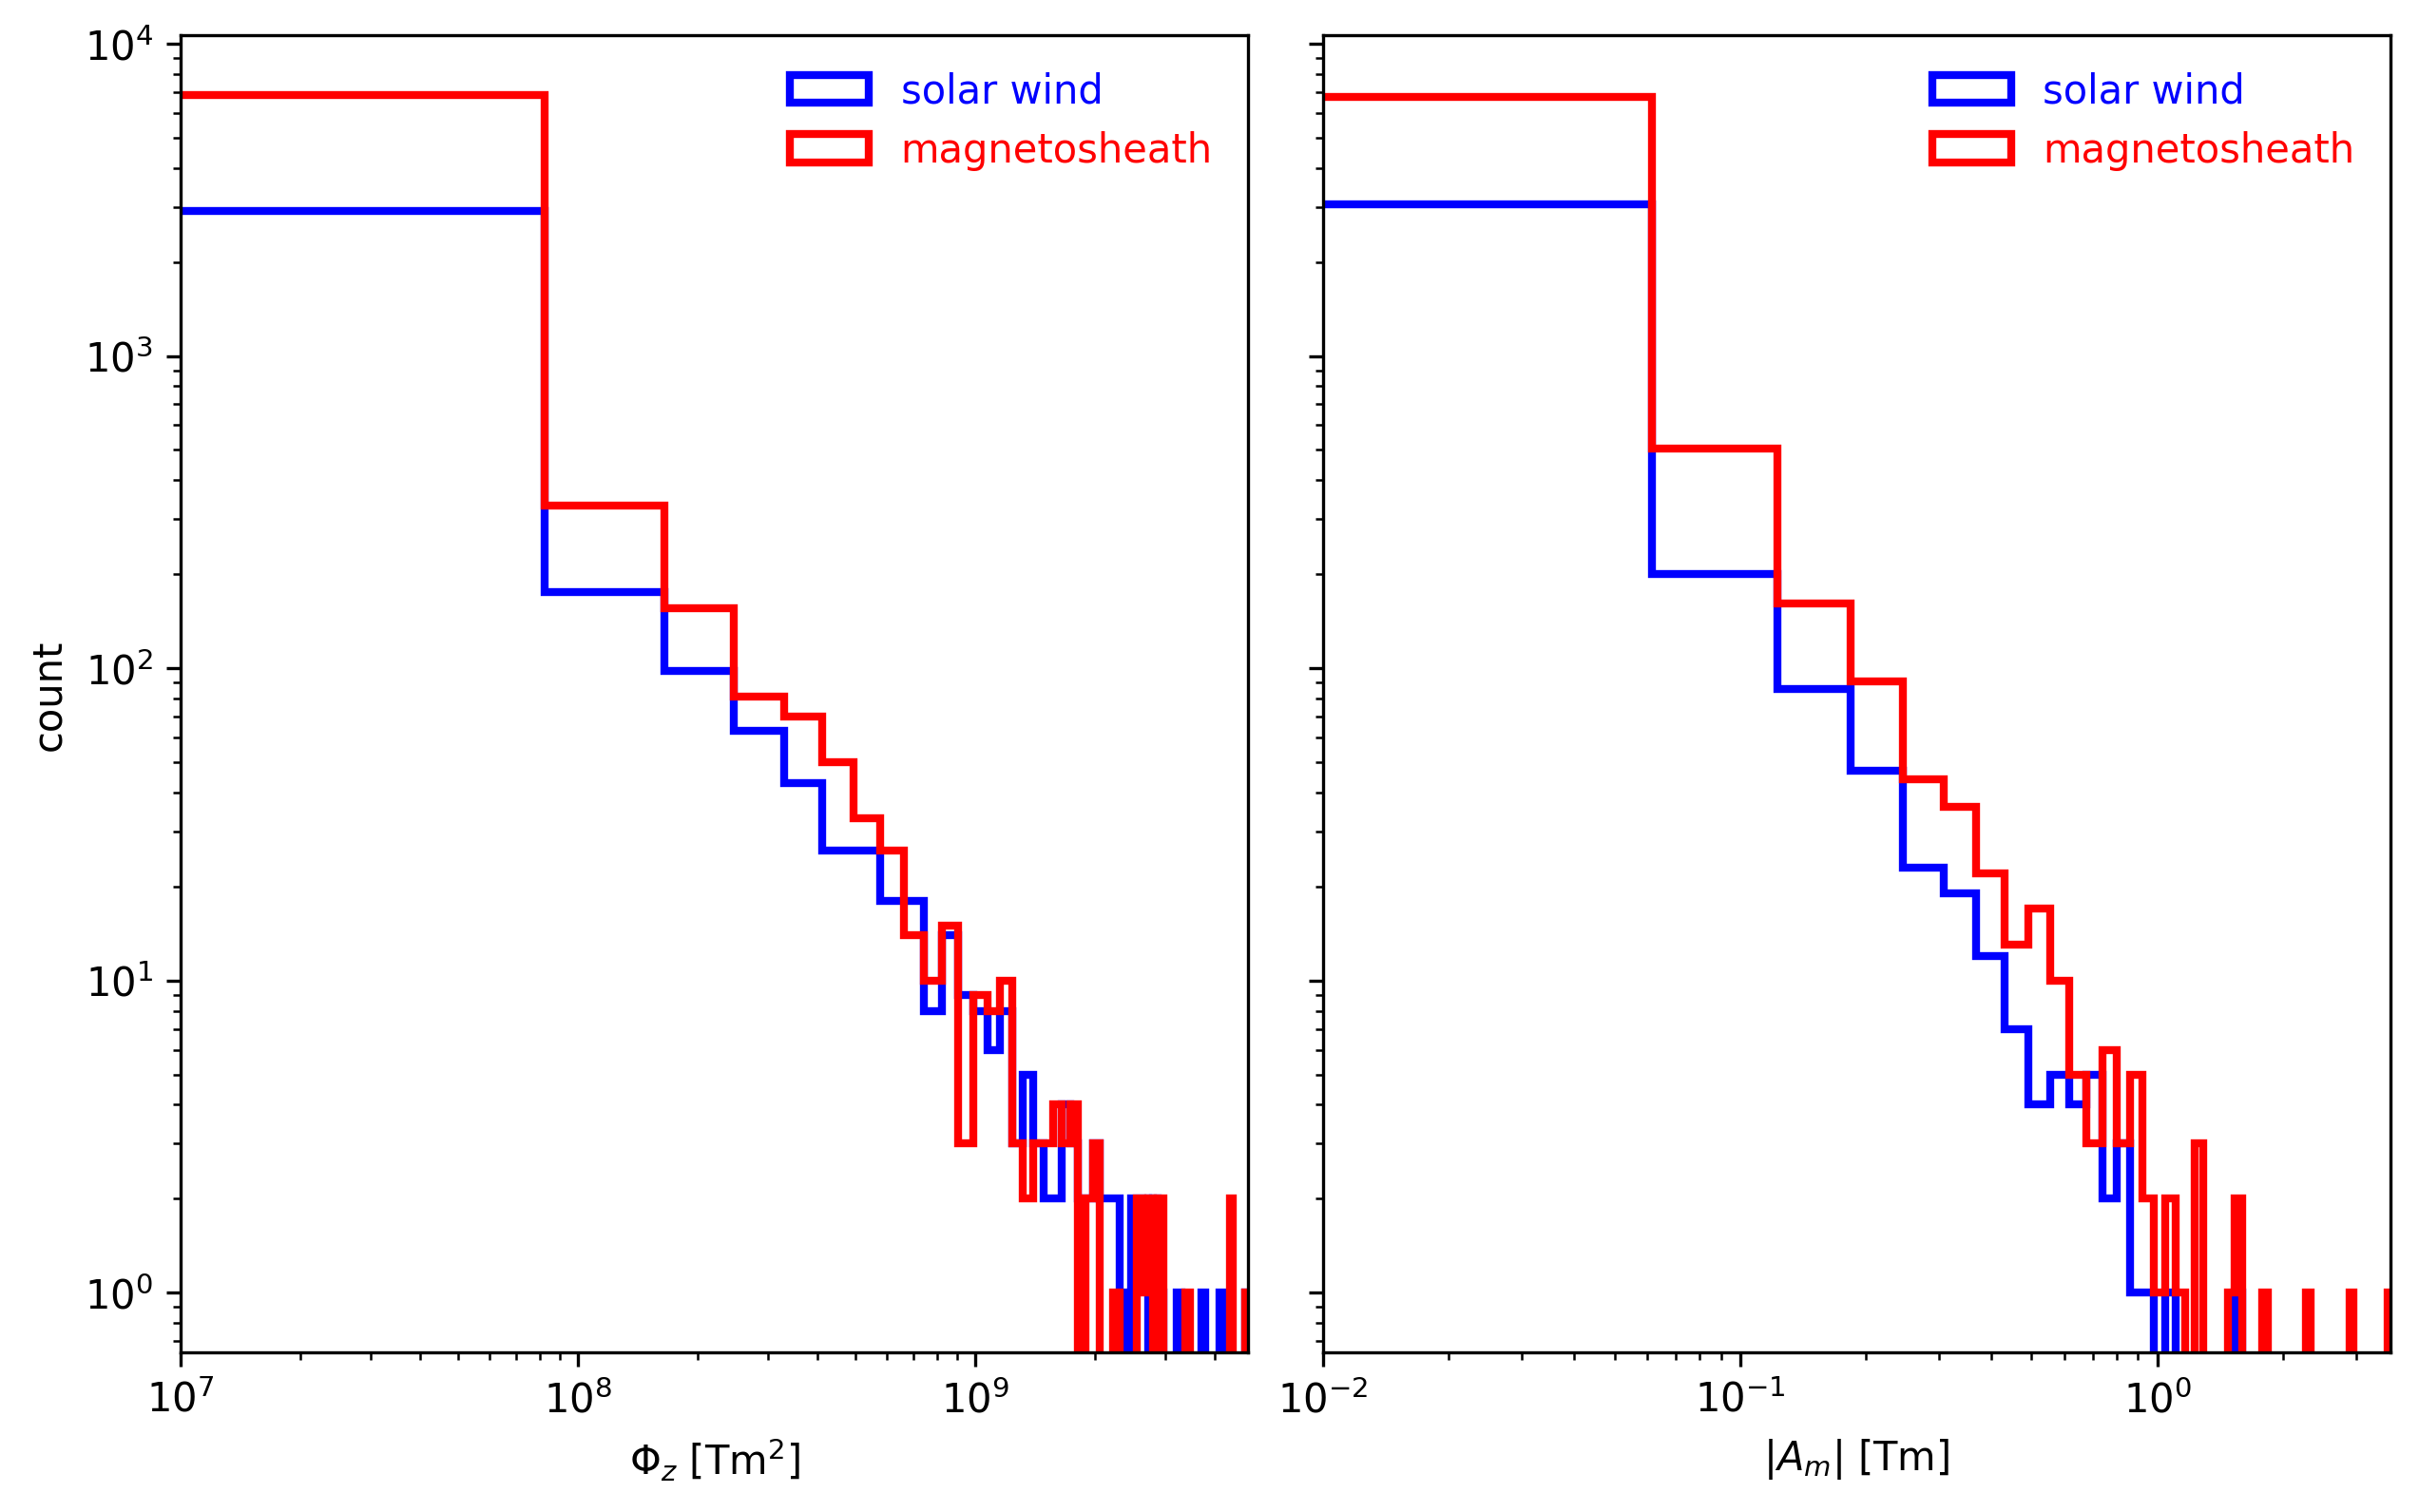
\includegraphics[width=\textwidth]{Figures/Histograms/histogram_flux_Am.png}
    \caption[Distributions of the axial flux and poloidal flux per unit length]{Distributions of the axial flux (left panel) and the poloidal flux per unit length (right panel) of events identified via the GS-based analysis. Blue lines are for solar wind events, and red lines for magnetosheath events.}
    \label{fig:histogram-flux}
\end{figure}

% Histogram of approximation to the helicity density \Phi_z * |Am|
\begin{figure}
    \centering
    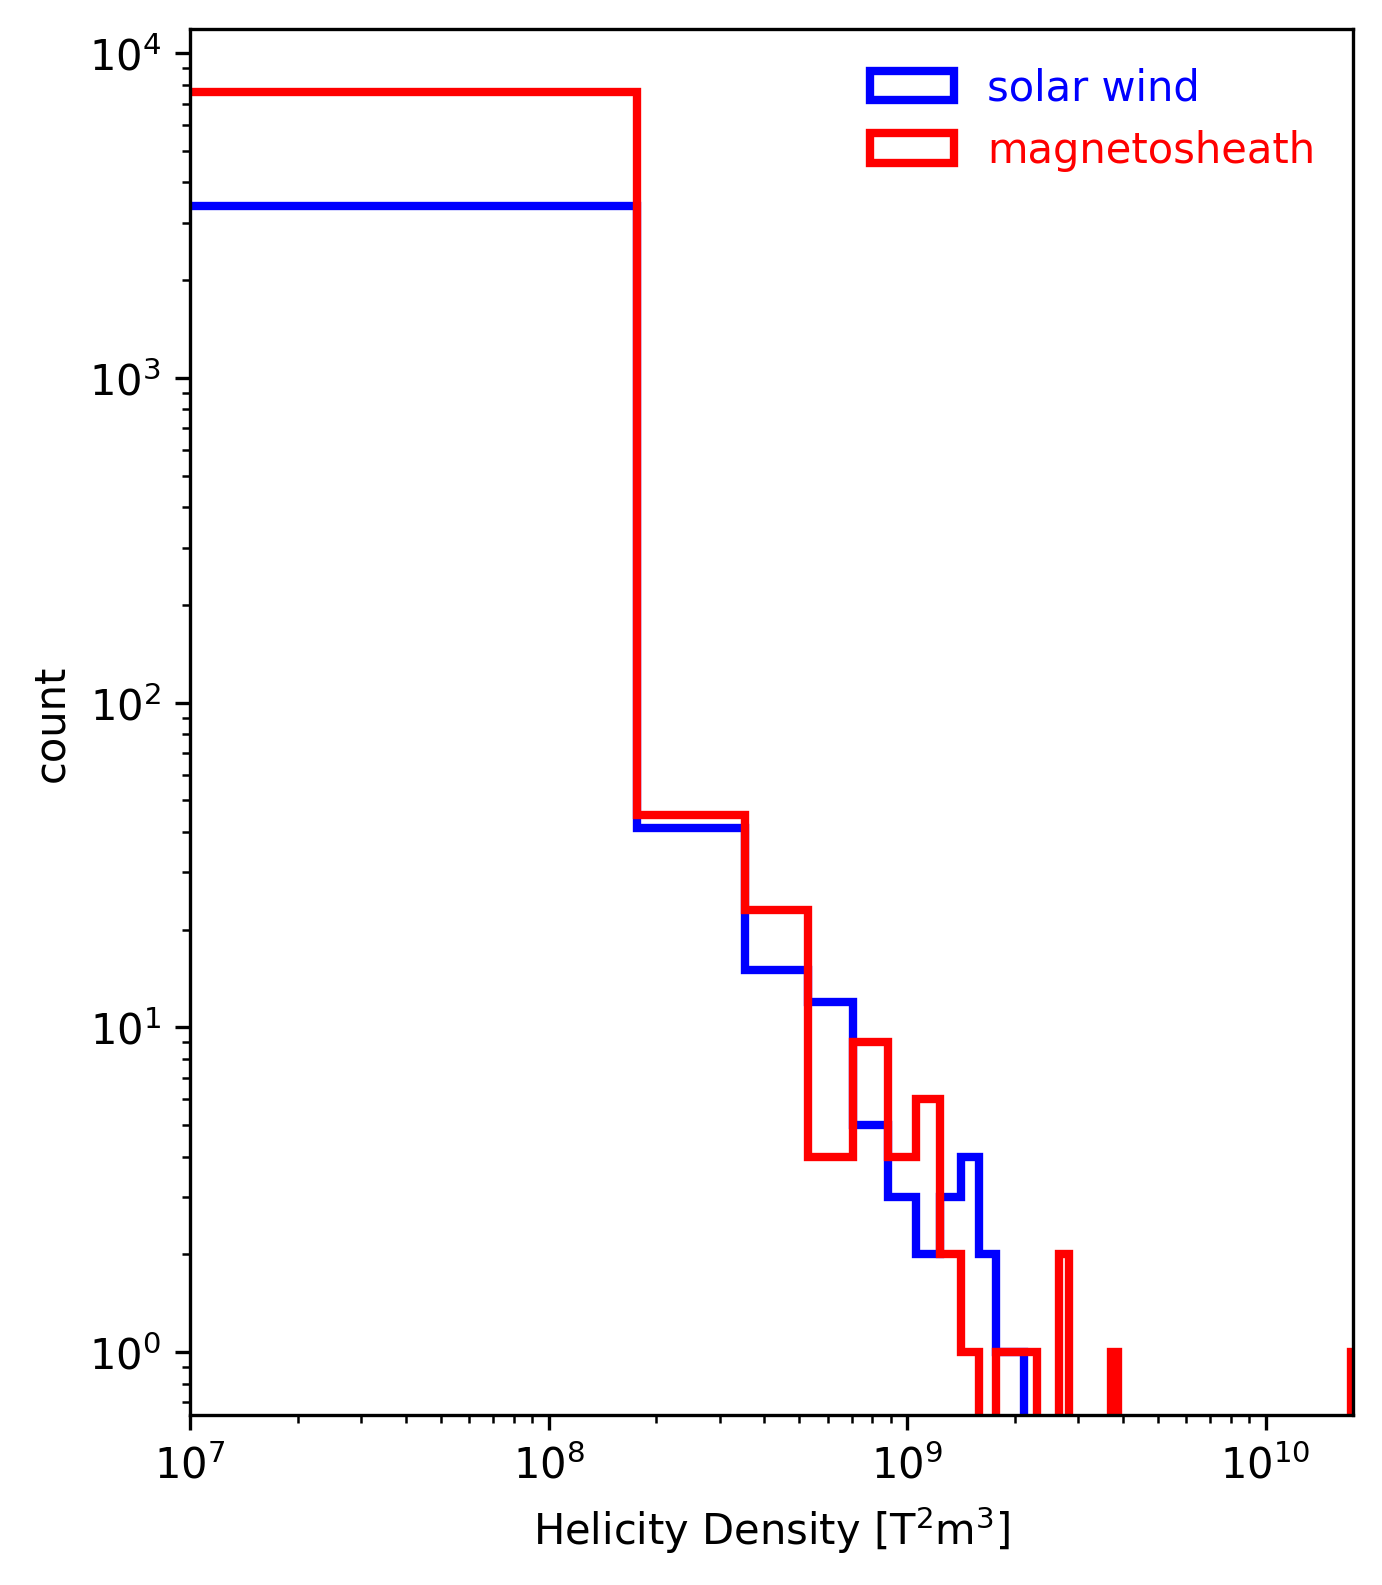
\includegraphics[width=0.6\textwidth]{Figures/Histograms/histogram_helicitydensity.png}
    \caption[Histograms for the approximation to the helicity density per unit length]{Histograms for the approximation to the helicity density per unit length of the events identified via the GS-based analysis for the solar wind (blue) and the magnetosheath (red).}
    \label{fig:histogram-helicitydensity}
\end{figure}

% 2D heatmaps
Figures \ref{fig:heatmap-solarwind} and \ref{fig:heatmap-magntosheath} display the 2D distributions of various parameters vs. the poloidal magnetic flux per unit length $|A_m|$ for events identified with the GS-based method. The distributions of a) average velocity, b) proton $\beta$, c) scale size, and d) the product of $<|B_y|>$ and one-half of the scale size versus $|A_m|$. The average value of $|A_m|$ in each bin (on the $x$-axis) are marked by red X's. The peaks in poloidal flux for all distributions in the magnetosheath are centered around $|A_m|=10^{-2}$ Tm, whereas in the solar wind this value is $|A_m|=10^-{3}$ Tm. For the scale size versus $|A_m|$ distribution, the is a larger range of events with smaller scale size and lower $|A_m|$ in the magnetosheath that in the solar wind. The peak for the distribution in the solar wind is near ($|A_m|=10^{-3}$ Tm, size=2$\times 10^4$ km), and for the magnetosheath it is close to ($|A_m|=10^{-2}$ Tm, size=$10^4$ km); thus, the magnetosheath is seen to experience larger flux with smaller-sized structures. These results complement the idea that the SFRs experience compression downstream of the bow shock.

\begin{figure}[ht!]
    \centering
    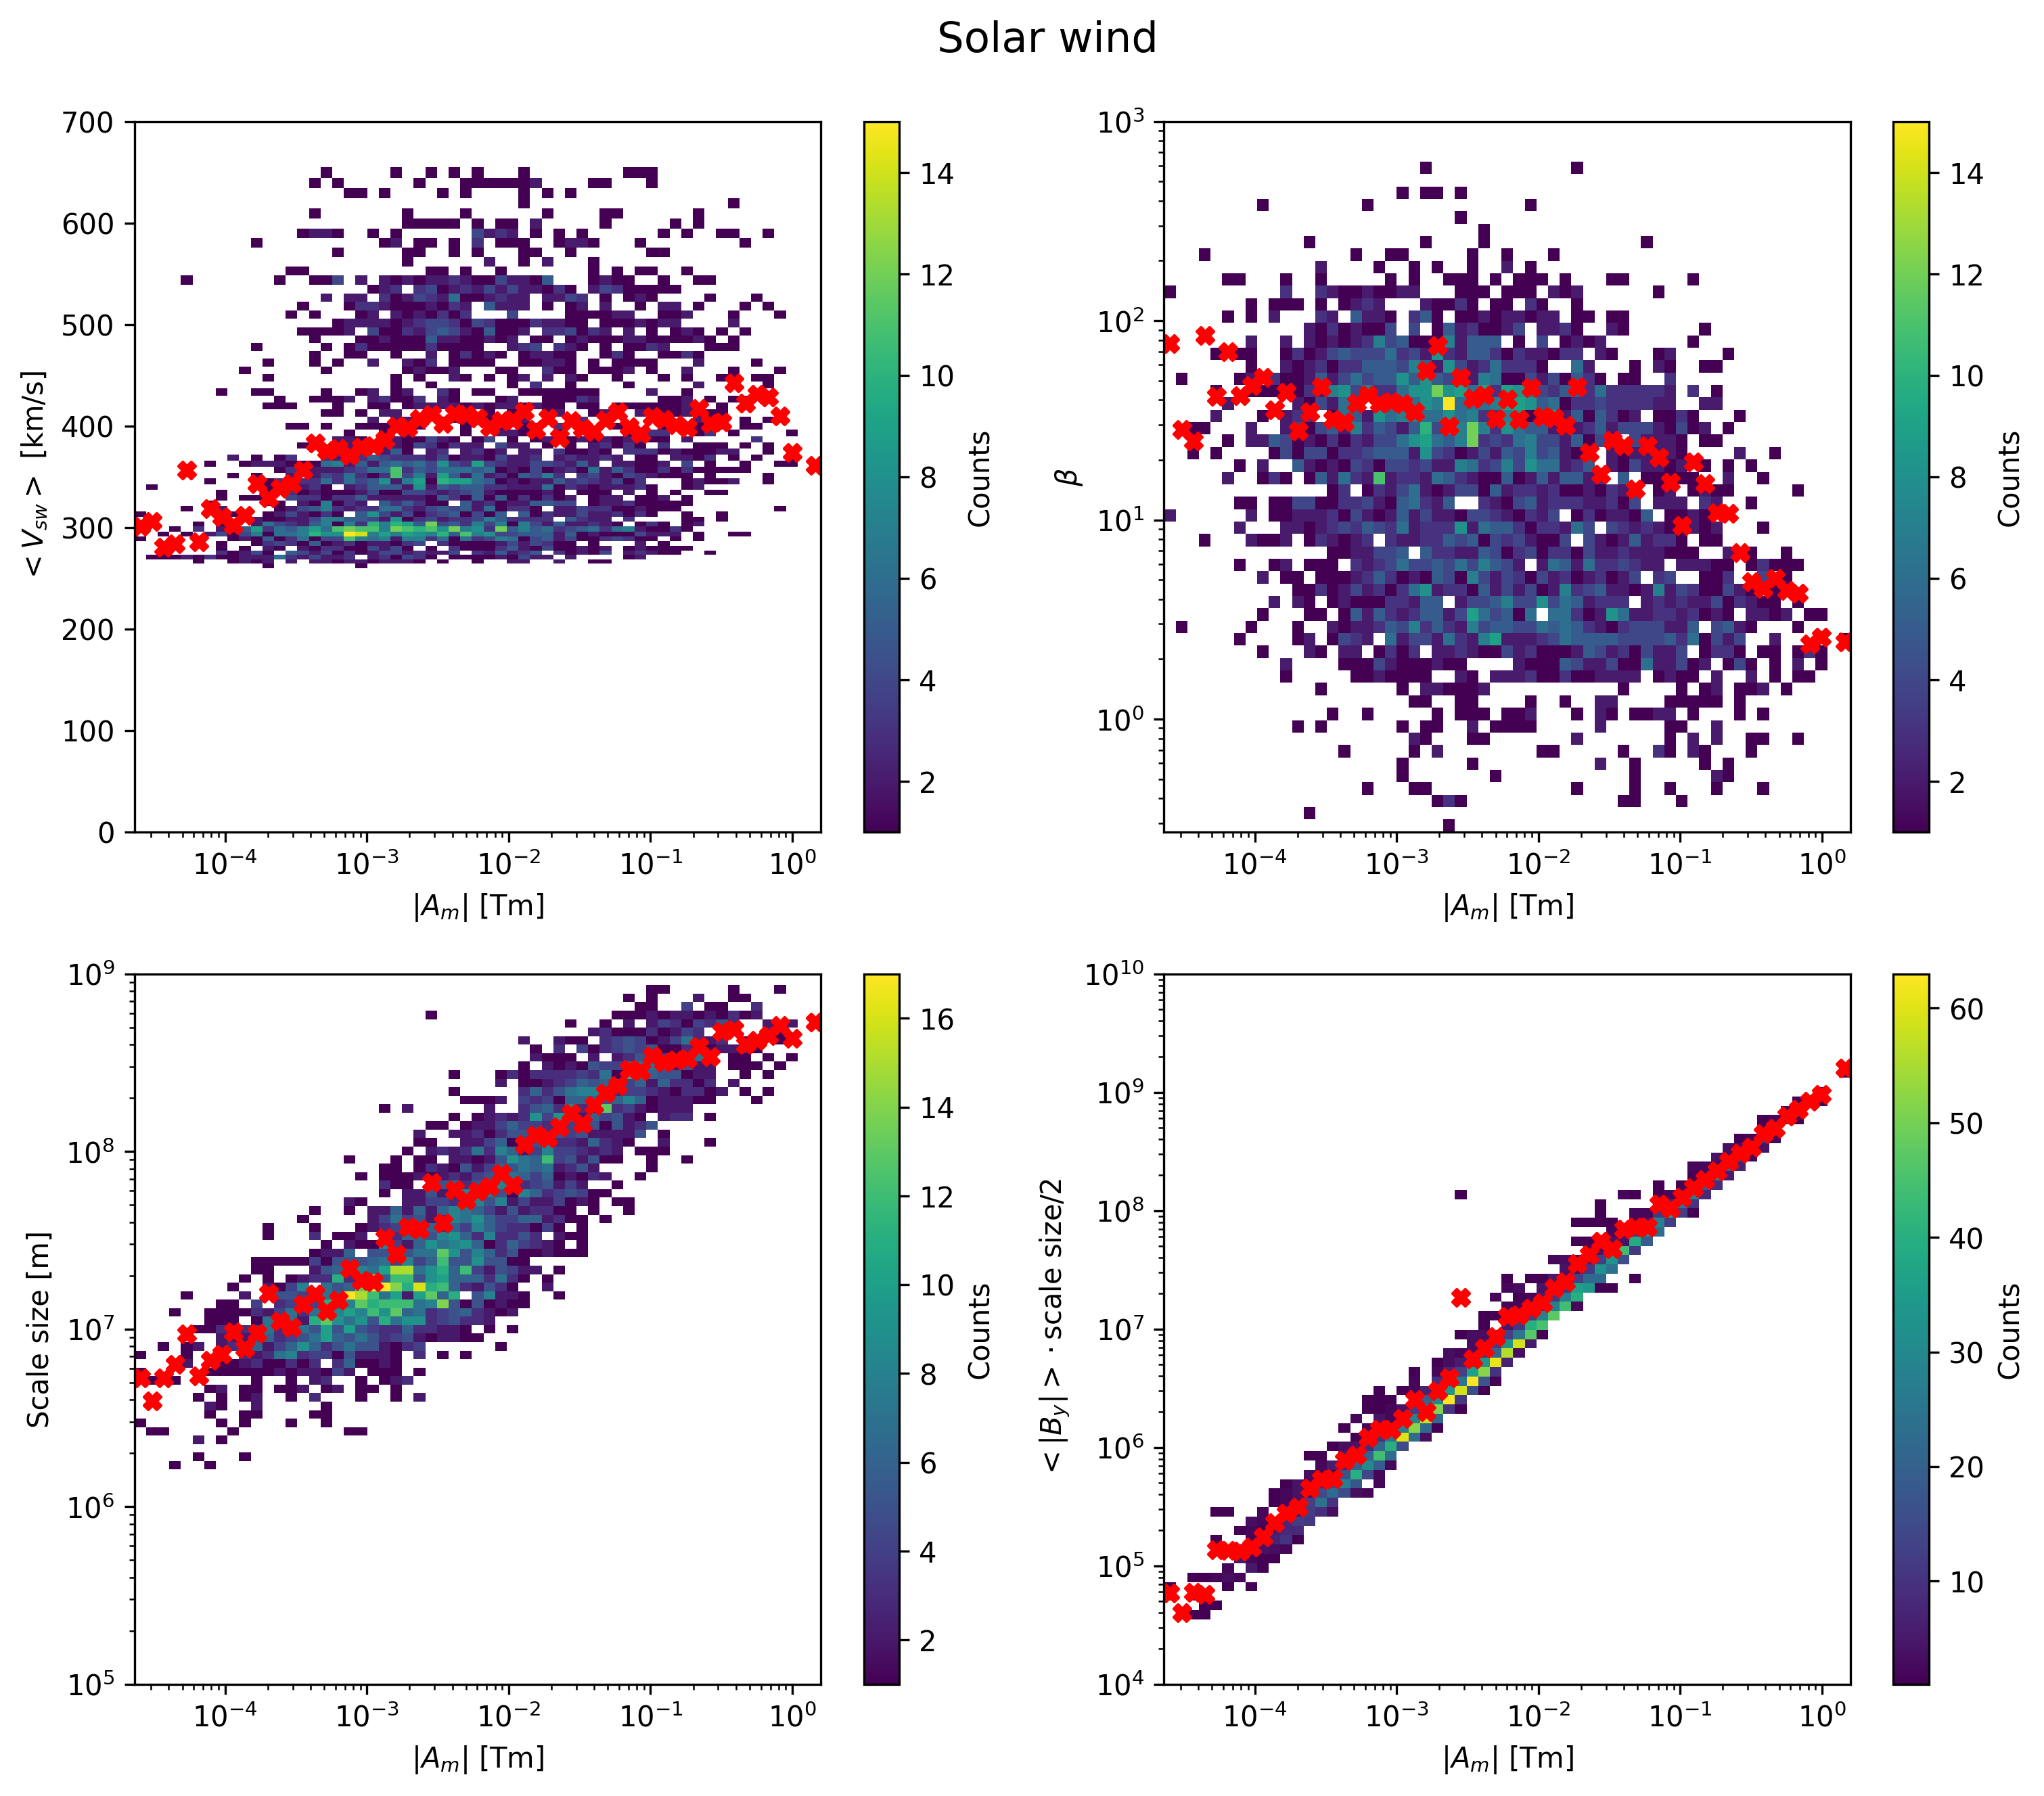
\includegraphics[width=\textwidth]{Figures/GS analysis/heatmap_solarwind.png}
    \caption[2D distributions of various parameters vs. $|A_m|$ in the solar wind]{2D distributions of a) average velocity, b) proton $\beta$, c) scale size, and d) the product of $<|B_y|>$ and one-half of the scale size versus the poloidal magnetic flux per unit length, for events identified with the GS-based method in the solar wind. The red X's mark the average value in each bin along the $x$-axis.}
    \label{fig:heatmap-solarwind}
\end{figure}

\begin{figure}[ht!]
    \centering
    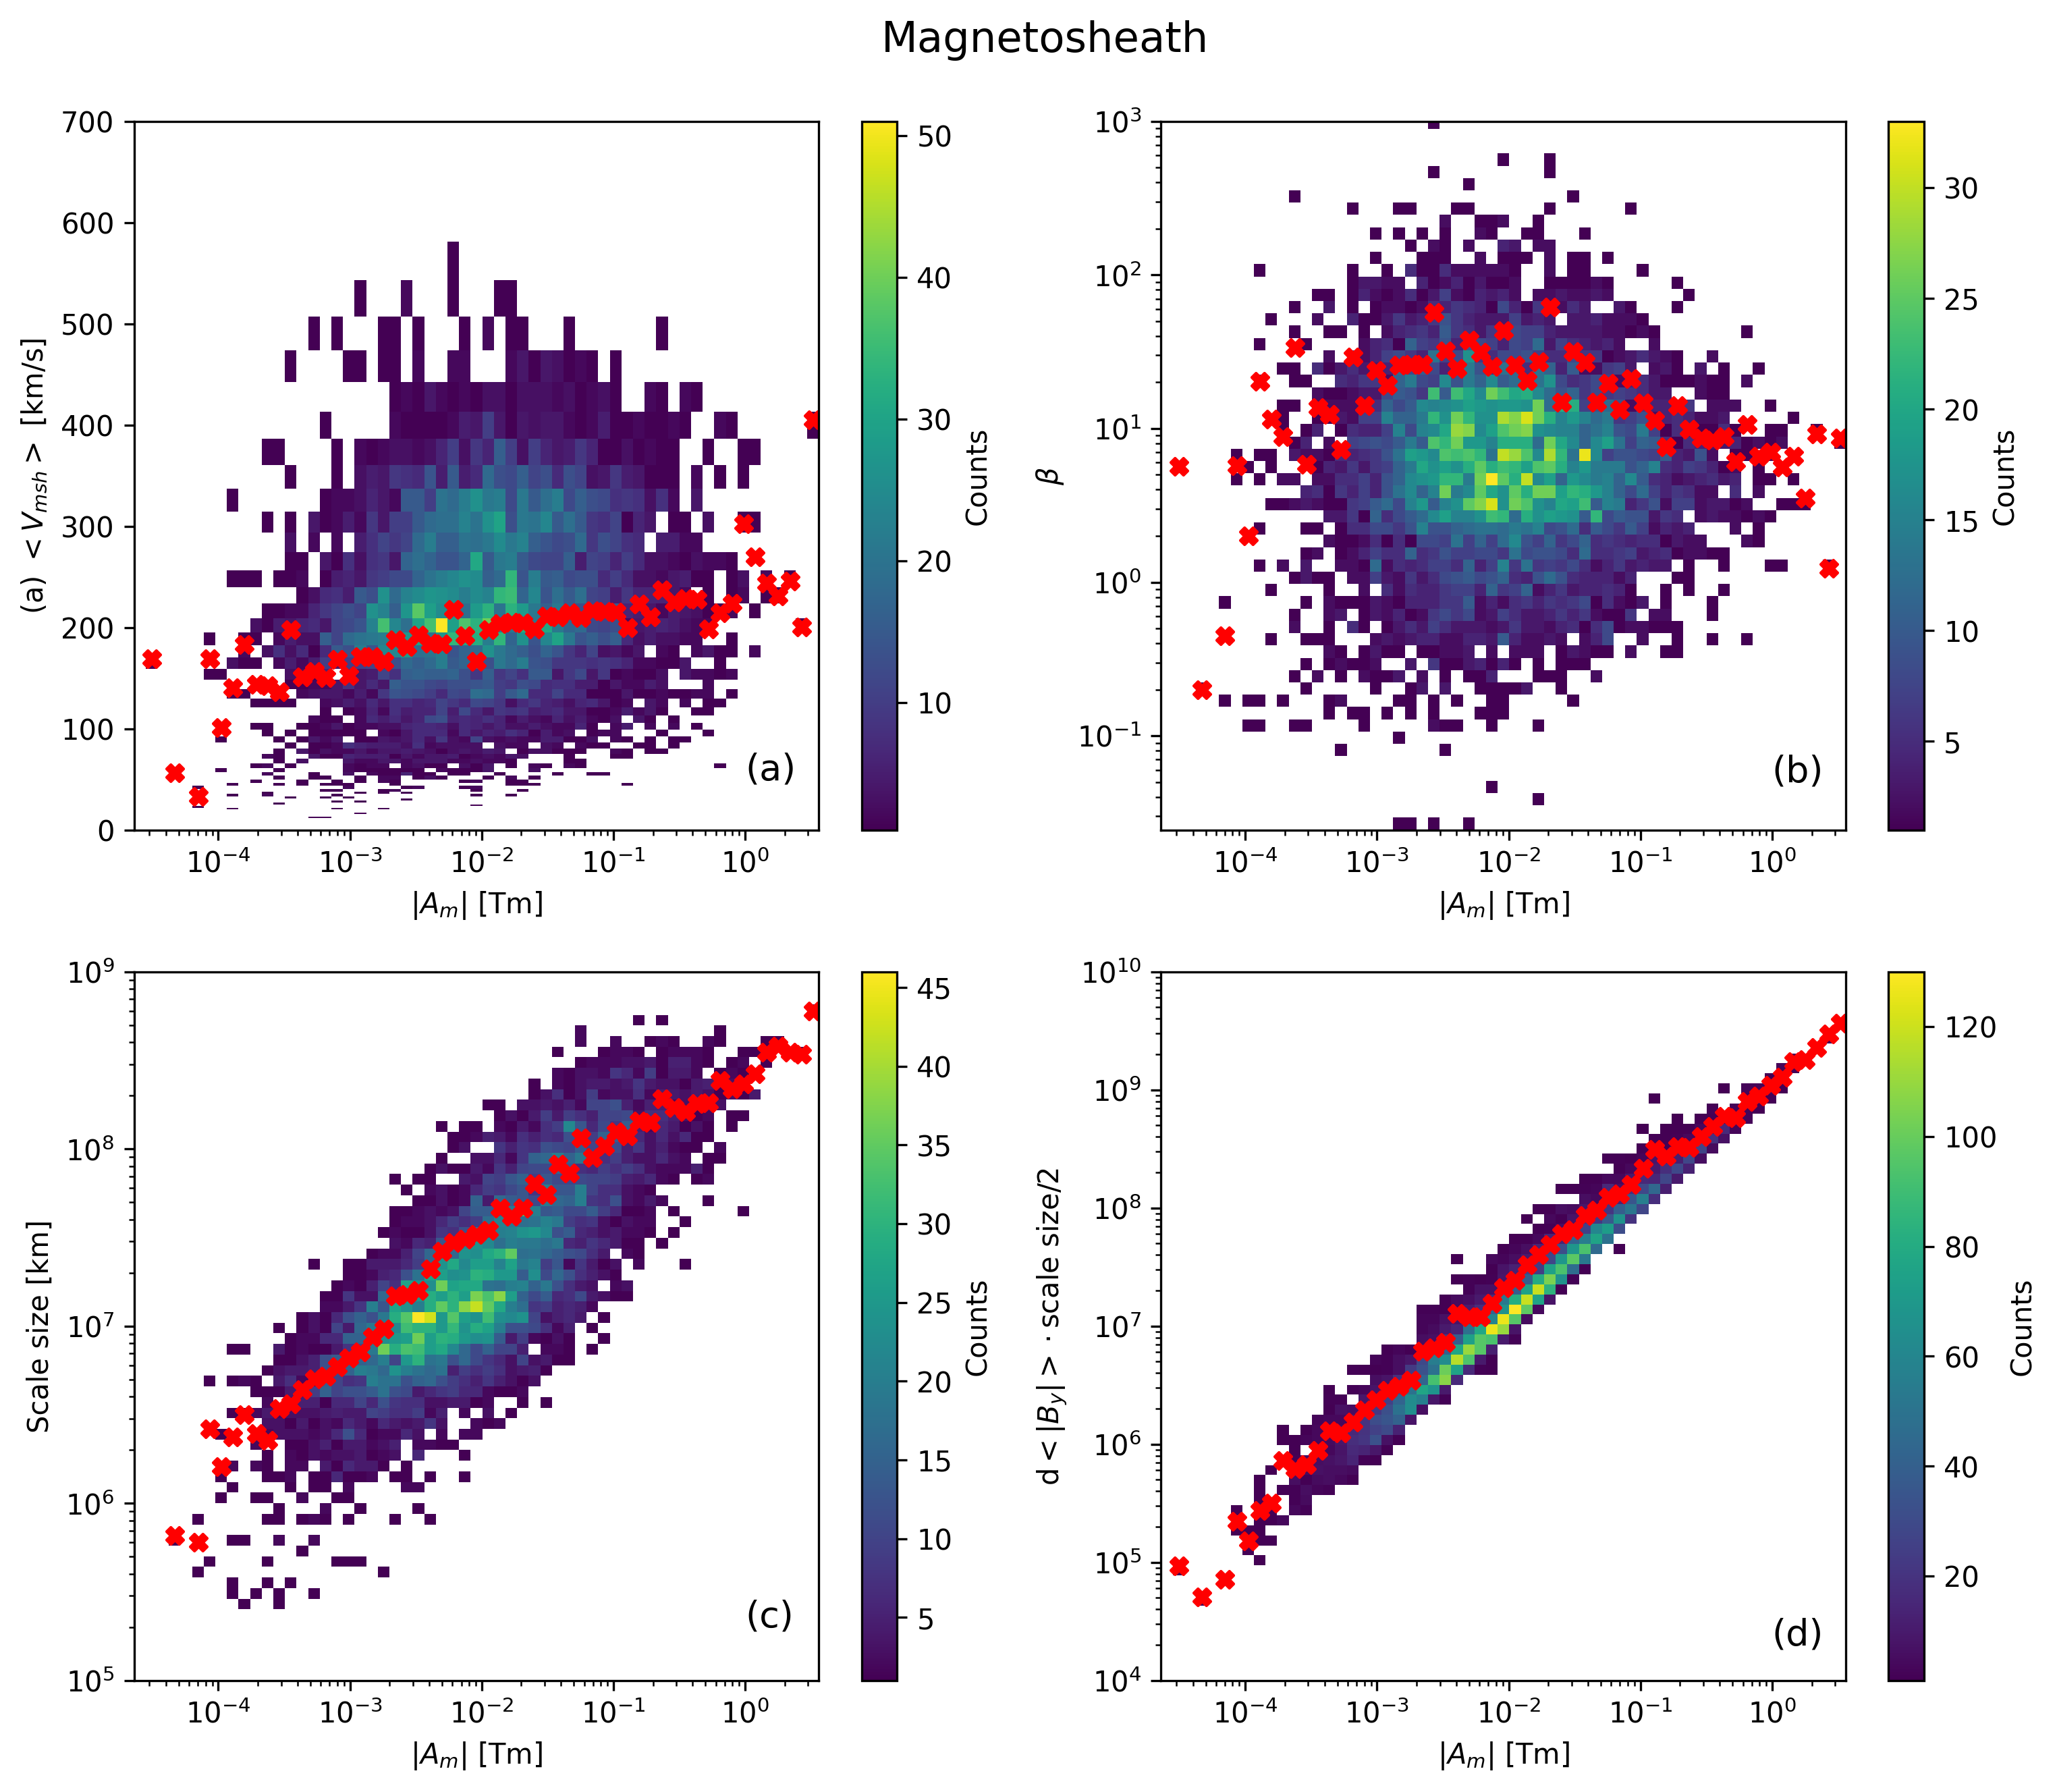
\includegraphics[width=\textwidth]{Figures/GS analysis/heatmap_magnetosheath.png}
    \caption[2D distributions of various parameters vs. $|A_m|$ in the magnetosheath]{2D distributions of a) average velocity, b) proton $\beta$, c) scale size, and d) the product of $<|B_y|>$ and one-half of the scale size versus the poloidal magnetic flux per unit length, for events identified with the GS-based method in the magnetosheath. The red X's mark the average value in each bin along the $x$-axis.}
    \label{fig:heatmap-magntosheath}
\end{figure}

\section{Wal\'en test and Alfv\'enicity}
As described in Section \ref{sec:GS-detection}, the Wal\'en test slope $w$ is used to further distinguish Alfv\'enic structures. Figure \ref{fig:walen-slope-20191109} shows the linear regression between $\mathbf{V_{sw}} - \mathbf{V_{HT}}$ and $\mathbf{V_A}$ during the event on 9 November 2019 during 9:53:10 - 9:54:36 UT. The Wal\'en slope $w=-0.09$ indicates that this event is a static flux rope-like structure, because the magnitude of the slope is less than 0.3.
\begin{figure}
    \centering
    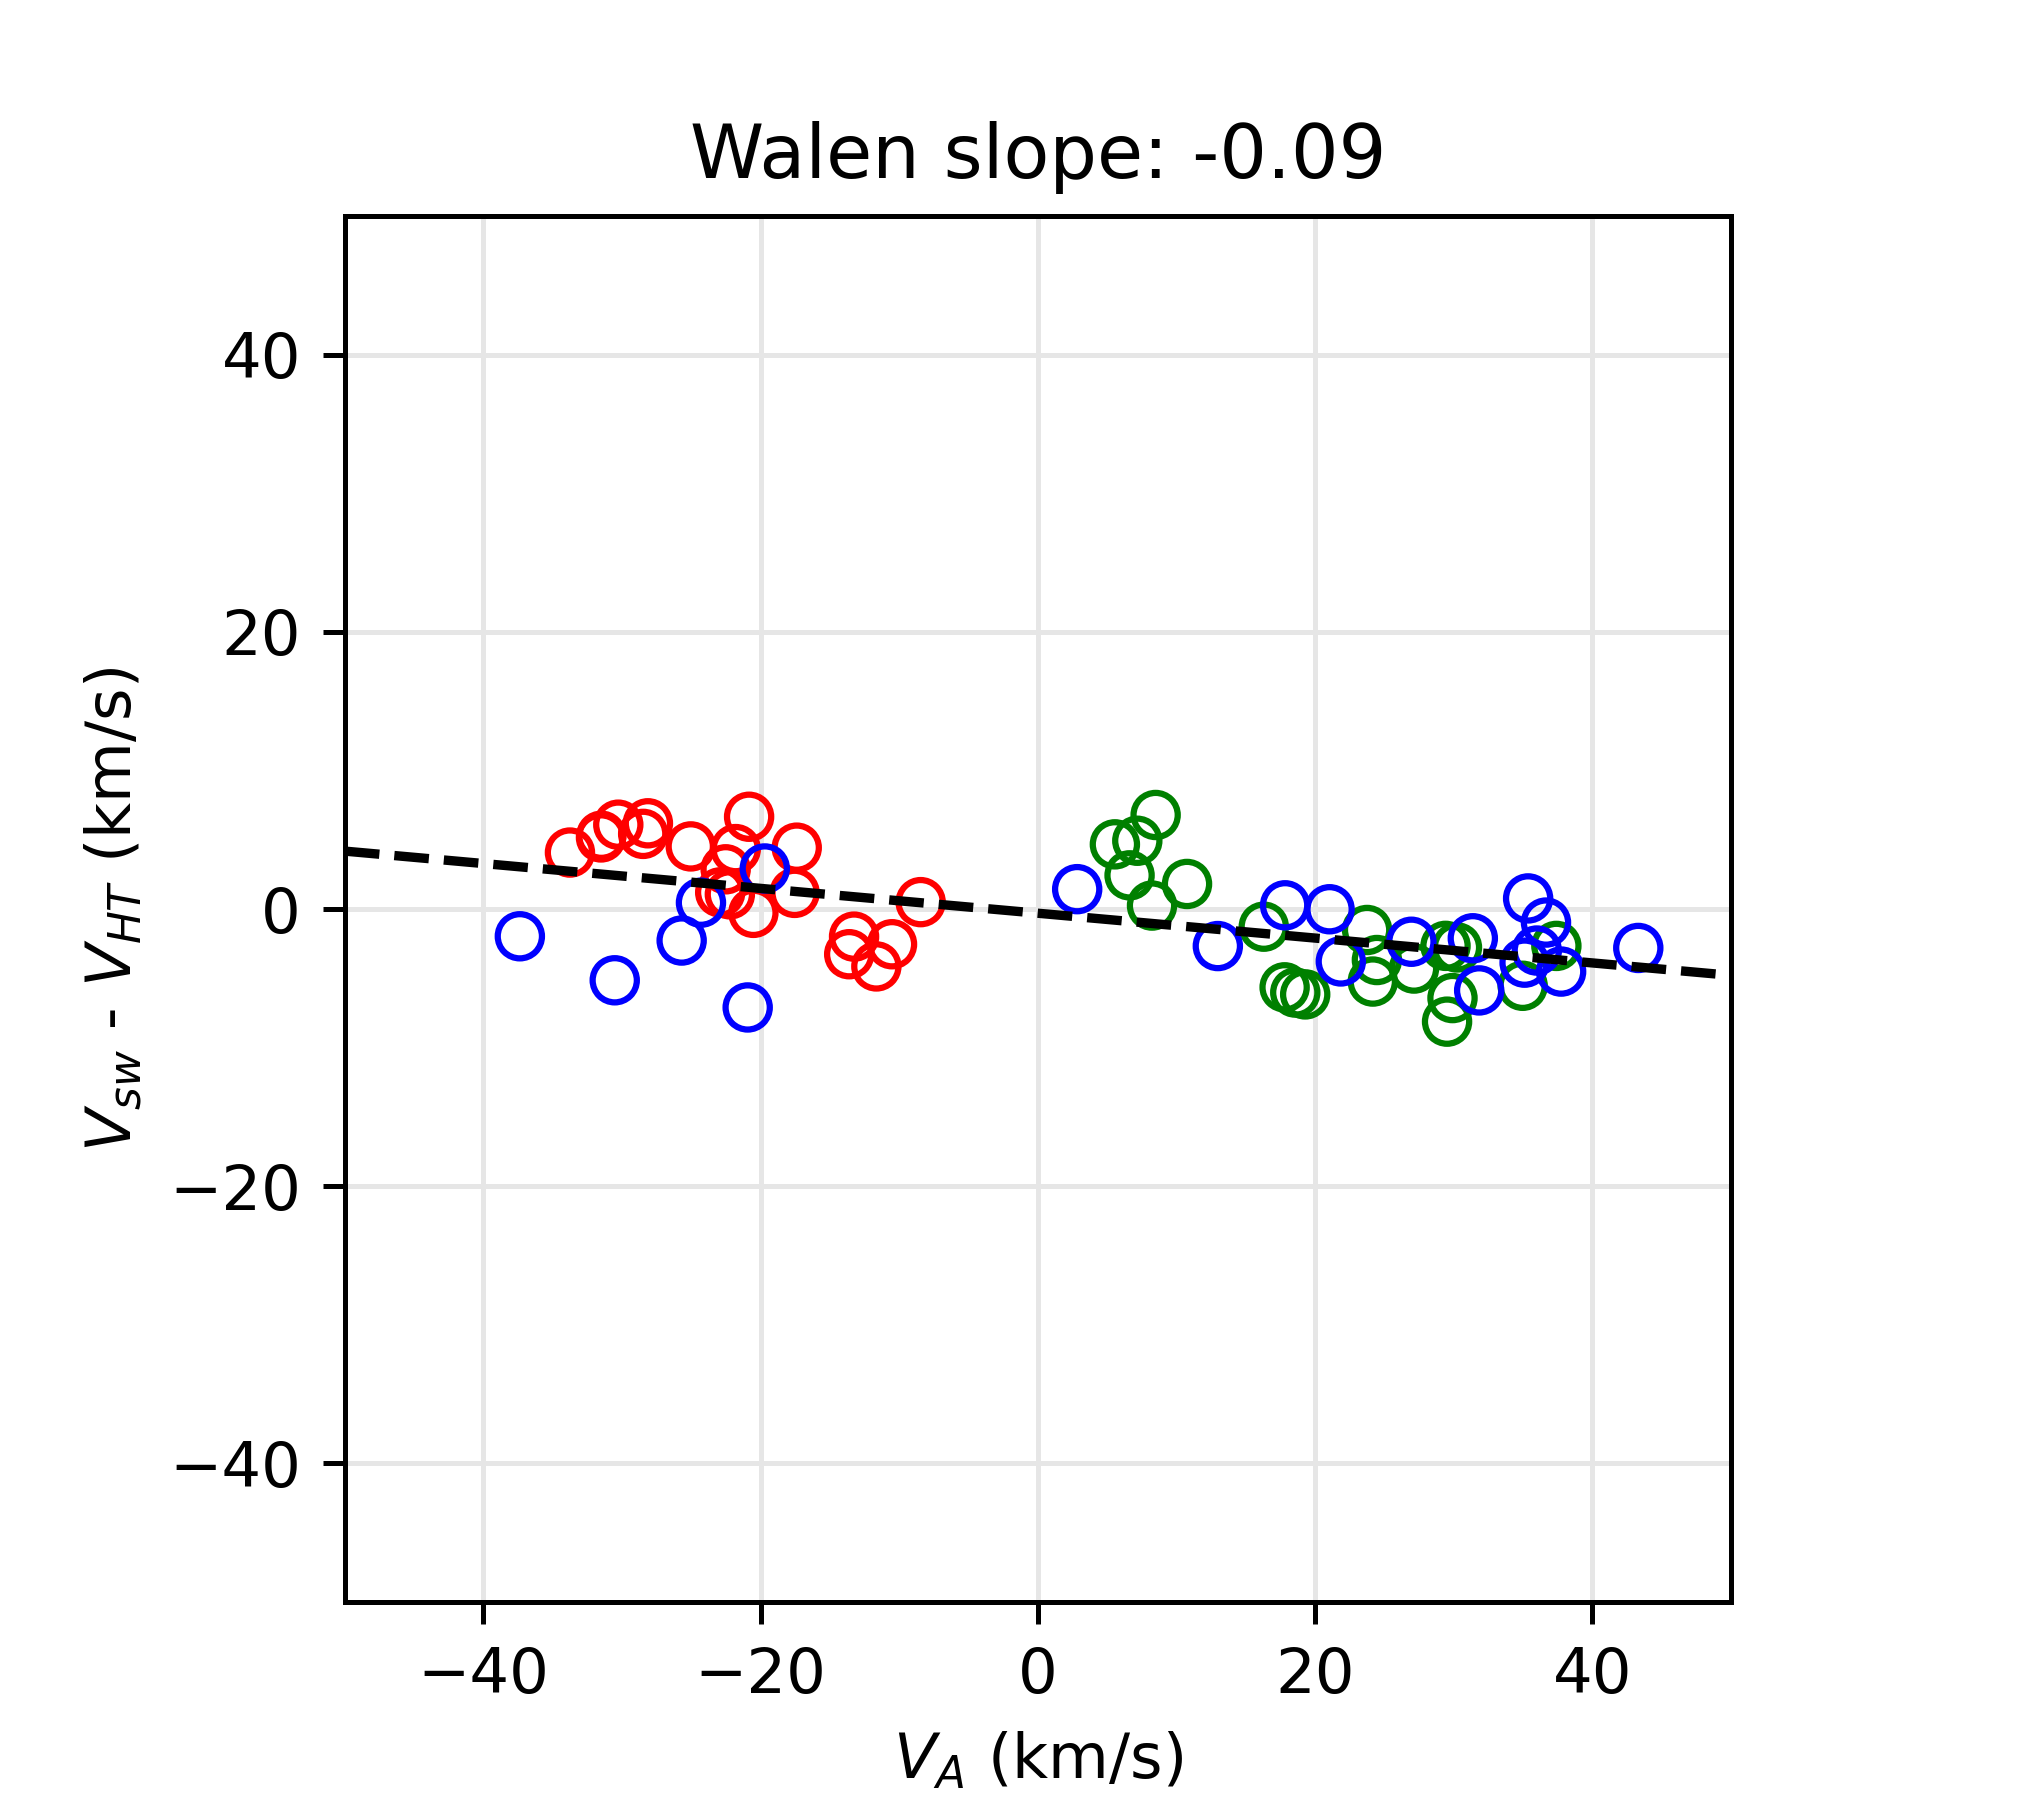
\includegraphics[width=\textwidth]{Figures/Reconstructions/MMS1_20191109095310_20191109095436_walen_relation.png}
    \caption[Plot of Wal\'en slope for 9 November 2019 9:53:10 - 9:54:36 UT]{Plot of $\mathbf{V_{sw}} - \mathbf{V_{HT}}$ and $\mathbf{V_A}$ for 9 November 2019 during 9:53:10 - 9:54:36 UT. The black dashed line is the linear regression between the two quantities. The slop of the line is the Wal\'en slope, as denoted on top. The red, green, and blue circles represent the $x-,y-,$ and $z-$ components of the velocities, respectively.}
    \label{fig:walen-slope-20191109}
\end{figure}

The distributions of the reduced cross helicity and residual energy for all identified events with the GS-based reconstruction identification algorithm are shown in Figure \ref{fig:mhd_histogram-GS}. Like Figure \ref{fig:mhd_histogram-wavelet} (in Section \ref{sec:wavelet-results}), Figure \ref{fig:mhd_histogram-GS} has a flatter distributions of reduced cross helicity $\sigma_c$ in the magnetosheath than in the solar wind. Unlike the analogous distributions in Figure \ref{fig:mhd_histogram-wavelet}, Figure \ref{fig:mhd_histogram-GS} shows that for the GS-based analysis result, there are nearly no events with $\sigma_r>0$. This is likely due to the intrinsic differences between the two methods. With the GS-based method, one can evaluate the Alfv\'enicity of the structures with the Wal\'en test slope. Table \ref{tab:walenTest-table} summarizes the classification of the events with the Wal\'en test slope. There is a slightly higher relative number of events with Wal\'en slope $|w|>0.3$ in the magnetosheath than in the solar wind. The majority (5088) of the 7689 events from the GS-based algorithm in the magnetosheath have Wal\'en test slopes $|w|\leq 0.3$, and 2601 events have Wal\'en slopes $|w|>0.3$. 1067 events of the 3476 GS-based algorithm events in the solar wind have $|w|>0.3$, which is a slightly lower proportion compared to that in the magnetosheath.

\begin{figure}
    \centering
    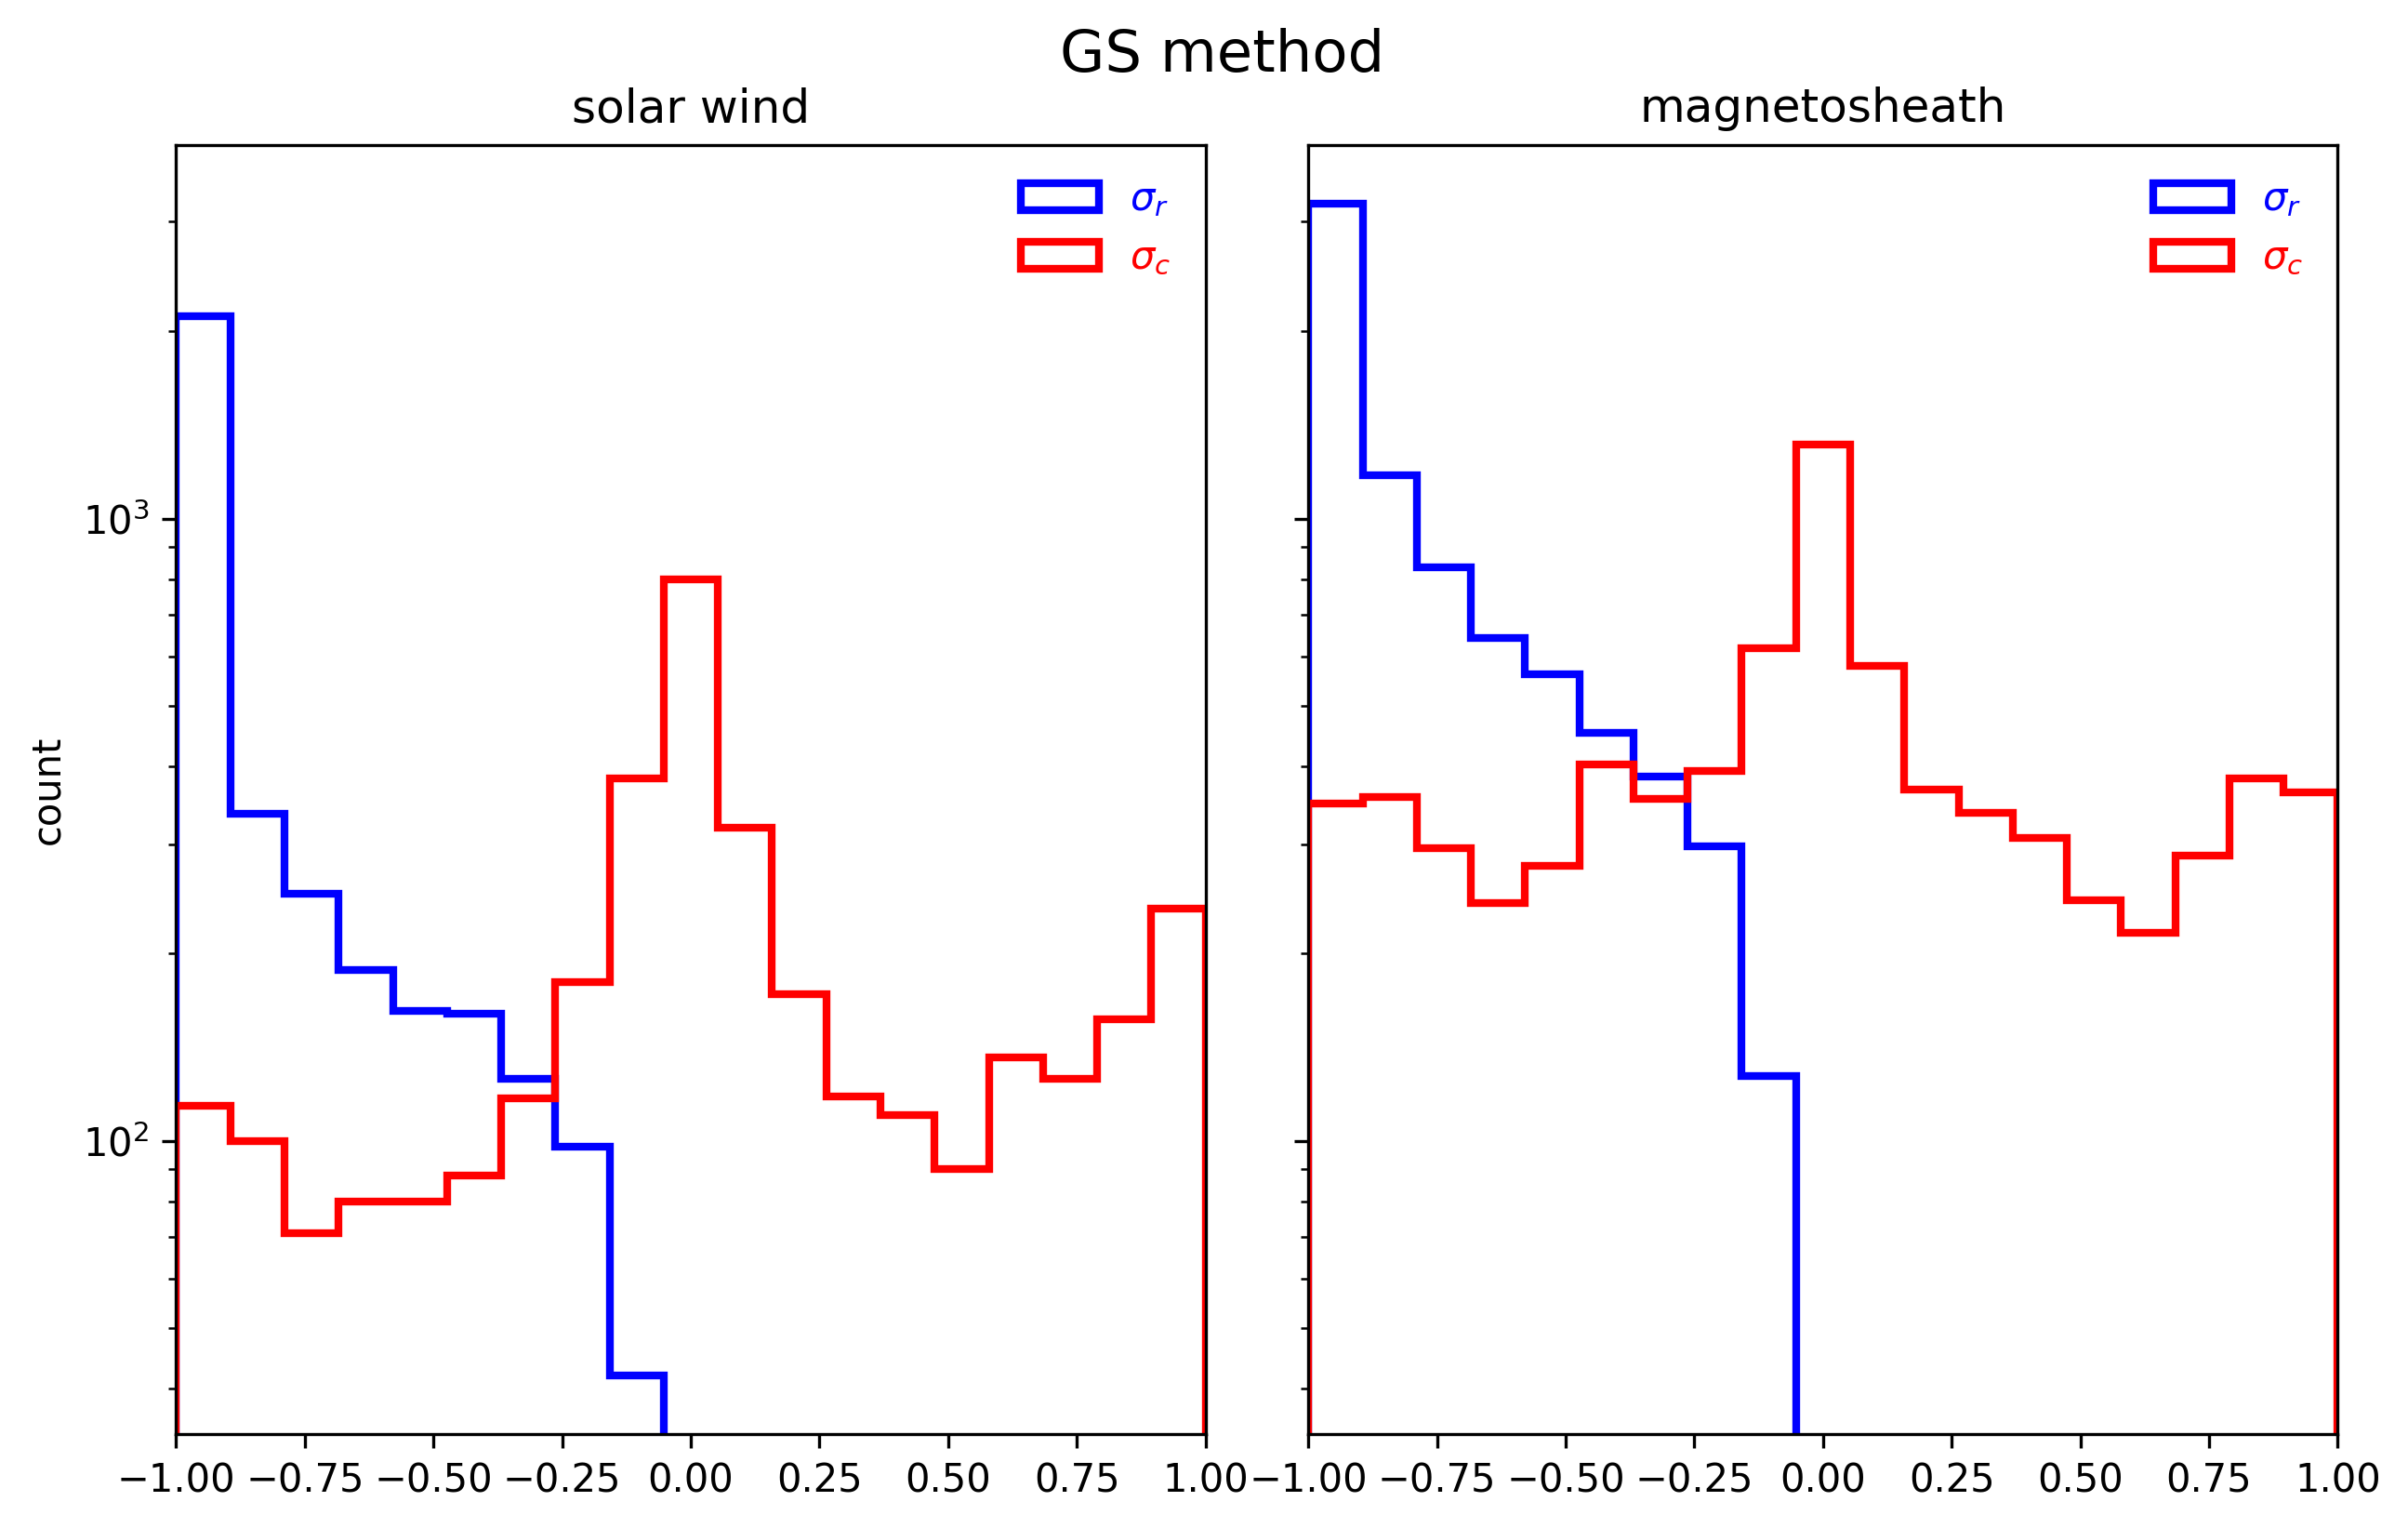
\includegraphics[width=\textwidth]{Figures/Histograms/sigr_sigc_GS.png}
    \caption[Reduced cross helicity and reduced residual energy for all events identified via GS-based reconstruction algorithm]{Histograms of reduced cross helicity $\sigma_c$ (red) and reduced residual energy $\sigma_r$ (blue) for all solar wind (left) and magnetosheath events (right) identified with the GS-based reconstruction identification algorithm.}
    \label{fig:mhd_histogram-GS}
\end{figure}

\begin{table}
    \caption{Events identified with the GS-based method meeting different Wal\'en test slope criteria.}
    \centering
    \begin{tabular}{rcc}
    \hline
                  & Solar wind & Magnetosheath \\
    \hline
    \textit{Total}& 3476 & 7689 \\
    $|w|\leq 0.3$ & 2409 & 5088 \\
    $|w|> 0.3$    & 1067 & 2601 \\
    \hline
\end{tabular}
    \label{tab:walenTest-table}
\end{table}

It can be seen that events with a high Alfv\'en Mach number (and thus proportionality constant $\alpha$) are more prominent in the magnetosheath. The distribution of the proportionality constant $\alpha$ partially represents the data in Tables \ref{tab:stats-GS-only} and \ref{tab:walenTest-table}. The mean $\alpha$ for events with $|w|\leq 0.3$ was 0.337 and 0.366 for the solar wind and magnetosheath, respectively. For $|w|>0.3$, the means had a greater difference at 0.059 and 0.139 for the respective regions. The median values for $\alpha$ in the solar wind were $7.575\times 10^{-3}$ for $|w|\leq 0.3$ and 0.297 for $|w|>0.3$. In the magnetosheath, the median values for $\alpha$ were 0.055 and 0.323 for $|w|\leq 0.3$ and $|w|>0.3$, respectively.

\begin{figure}
    \centering
    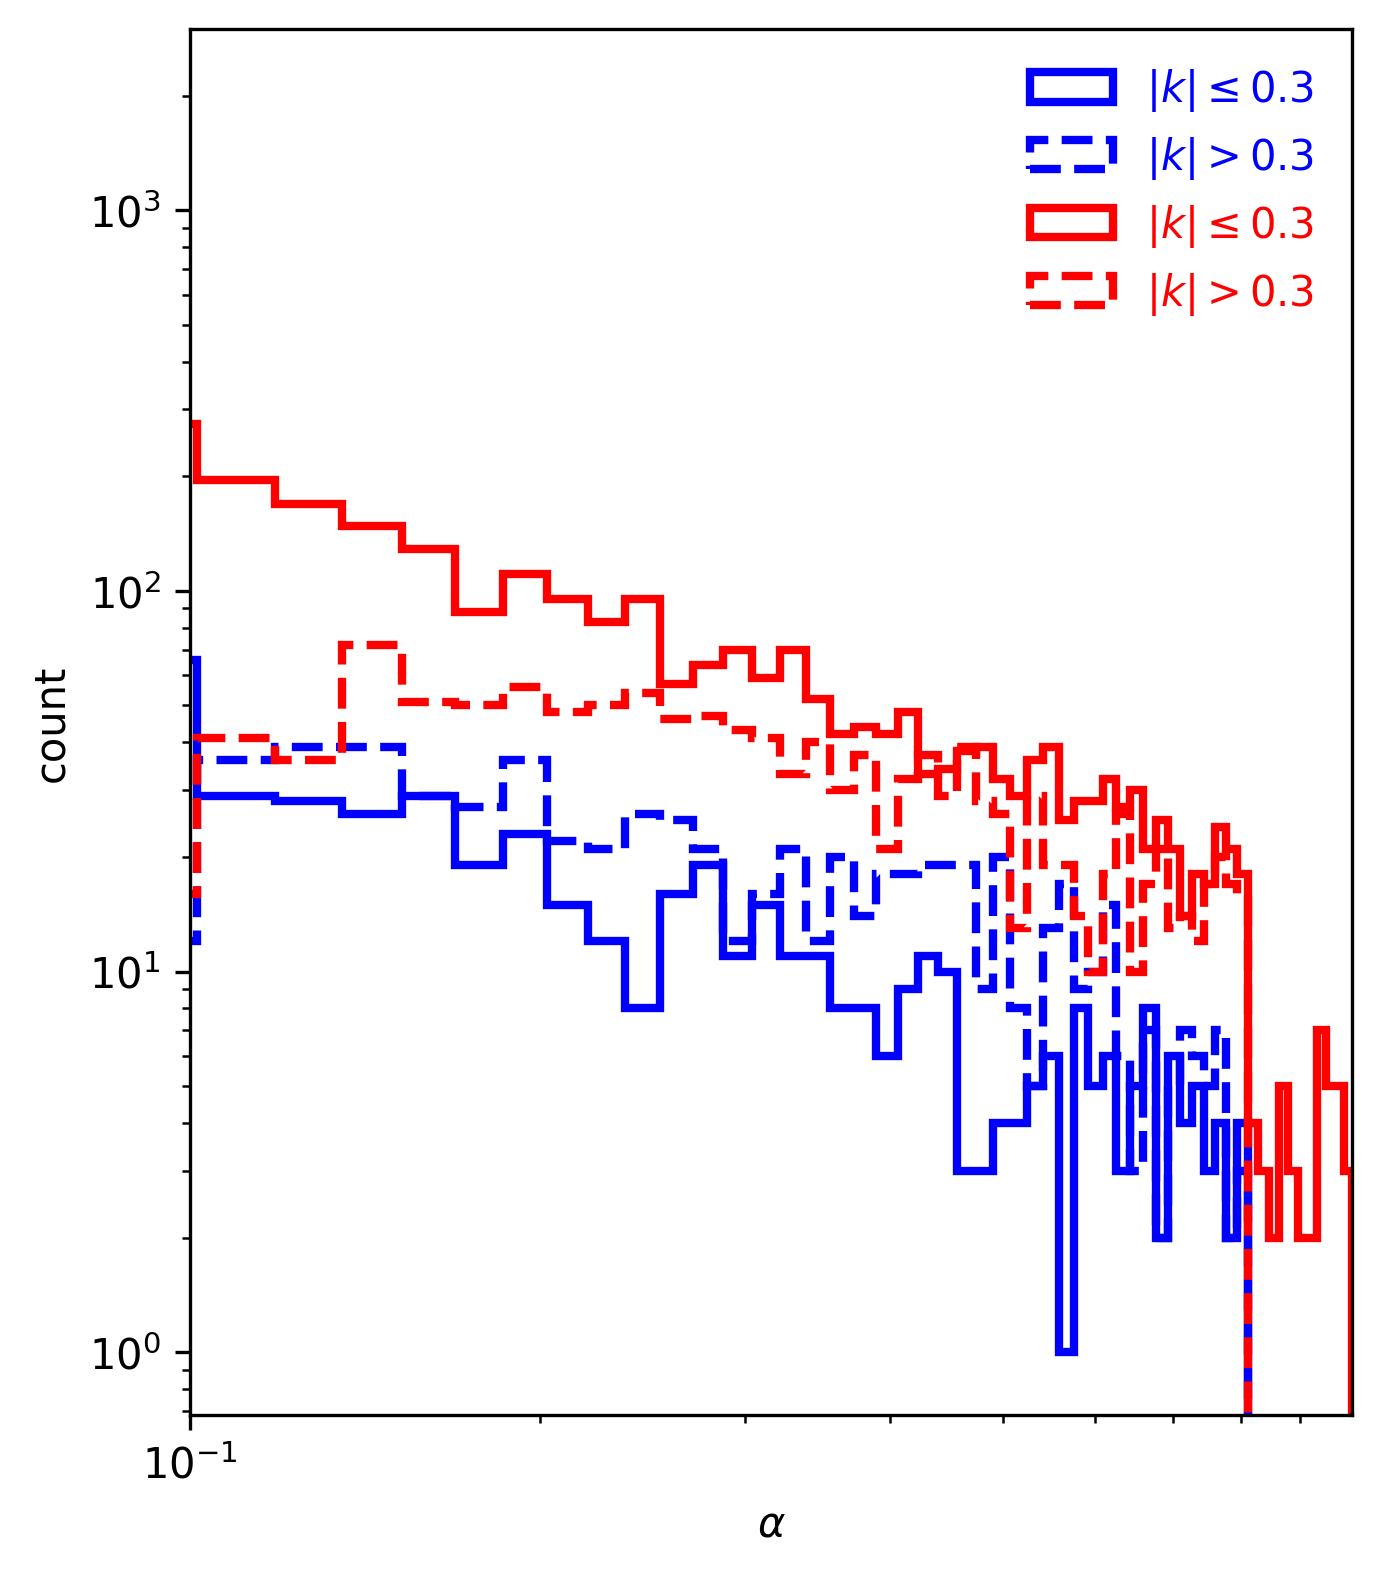
\includegraphics[width=0.6\textwidth]{Figures/Histograms/histogram_alpha.png}
    \caption[Histograms for proportionality constant $\alpha = \langle M_A \rangle^2$]{Histograms for proportionality constant $\alpha = \langle M_A \rangle^2$ of events identified via GS analysis. For this histogram, blue lines are solar wind events, and red lines are magnetosheath events. Solid lines represent events with a Wal\'en slope $|w|\leq 0.3$ and dashed lines represent events with $|w|> 0.3$.}
    \label{fig:histogram-alpha}
\end{figure}

Figure \ref{fig:walen-crosshelicity} shows the Wal\'en test slope versus the reduced cross helicity for all of the events identified via GS analysis. Each circle represents an event, with the size of the circle corresponding to the magnitude of the poloidal flux per unit length. It can be seen that in the solar wind, the events with a larger magnitude of poloidal flux have low cross helicity (close to zero), whereas in the magnetosheath the events with larger poloidal flux are seen closer to $\pm$1. The trend between the two quantities appears closely to a diagonal line, indicating that they are inherently related. \cite{Chen:2022} found a similar relation; however, beyond the connection to Alfv\'enicity, the physical correlation between the Wal\'en test slope and reduced cross helicity has not been determined.

\begin{figure}
    \centering
    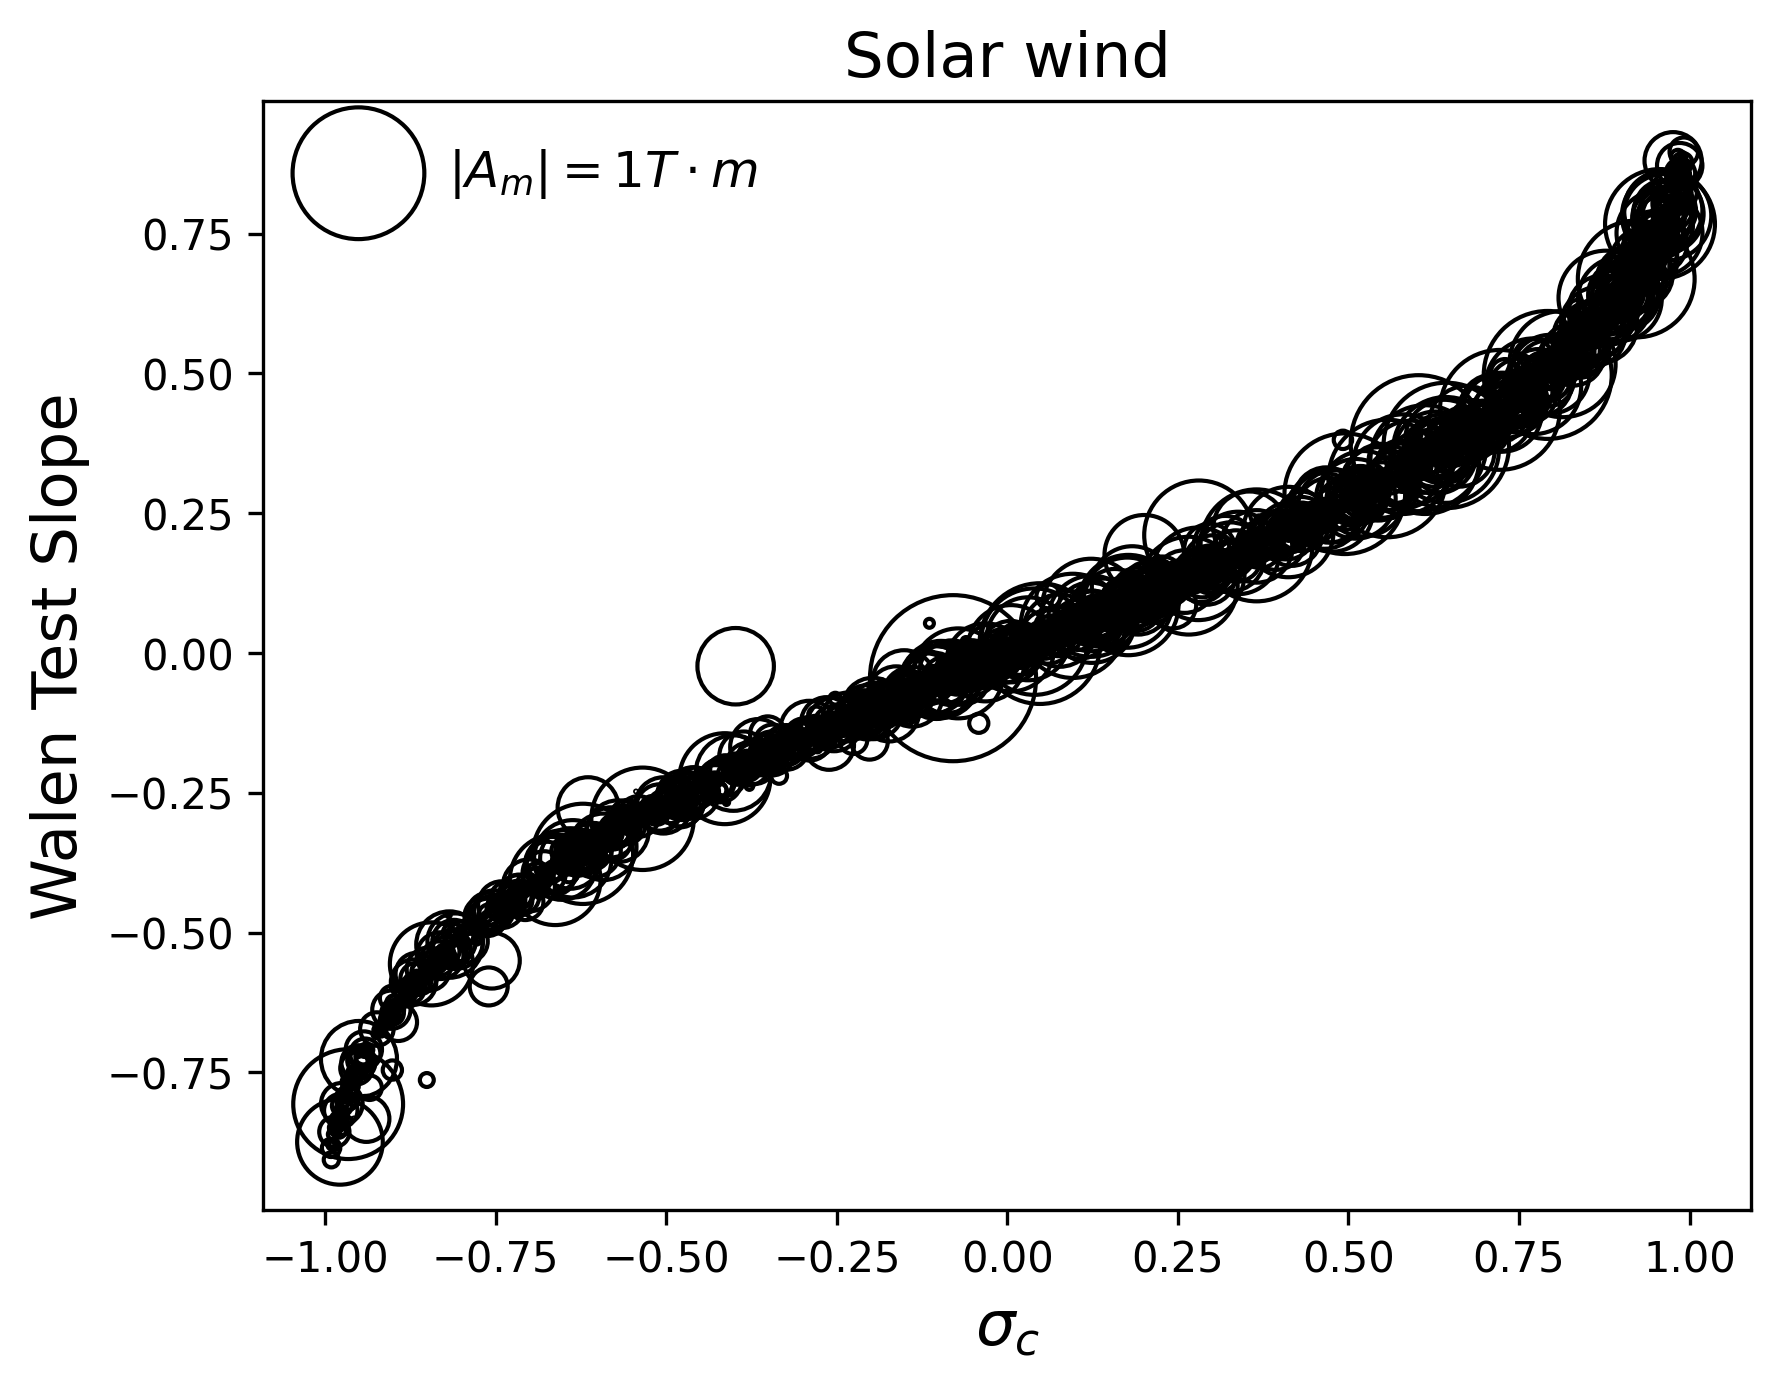
\includegraphics[width=0.7\textwidth]{Figures/GS analysis/walenTest_vs_crosshelicity_solarwind.png}
    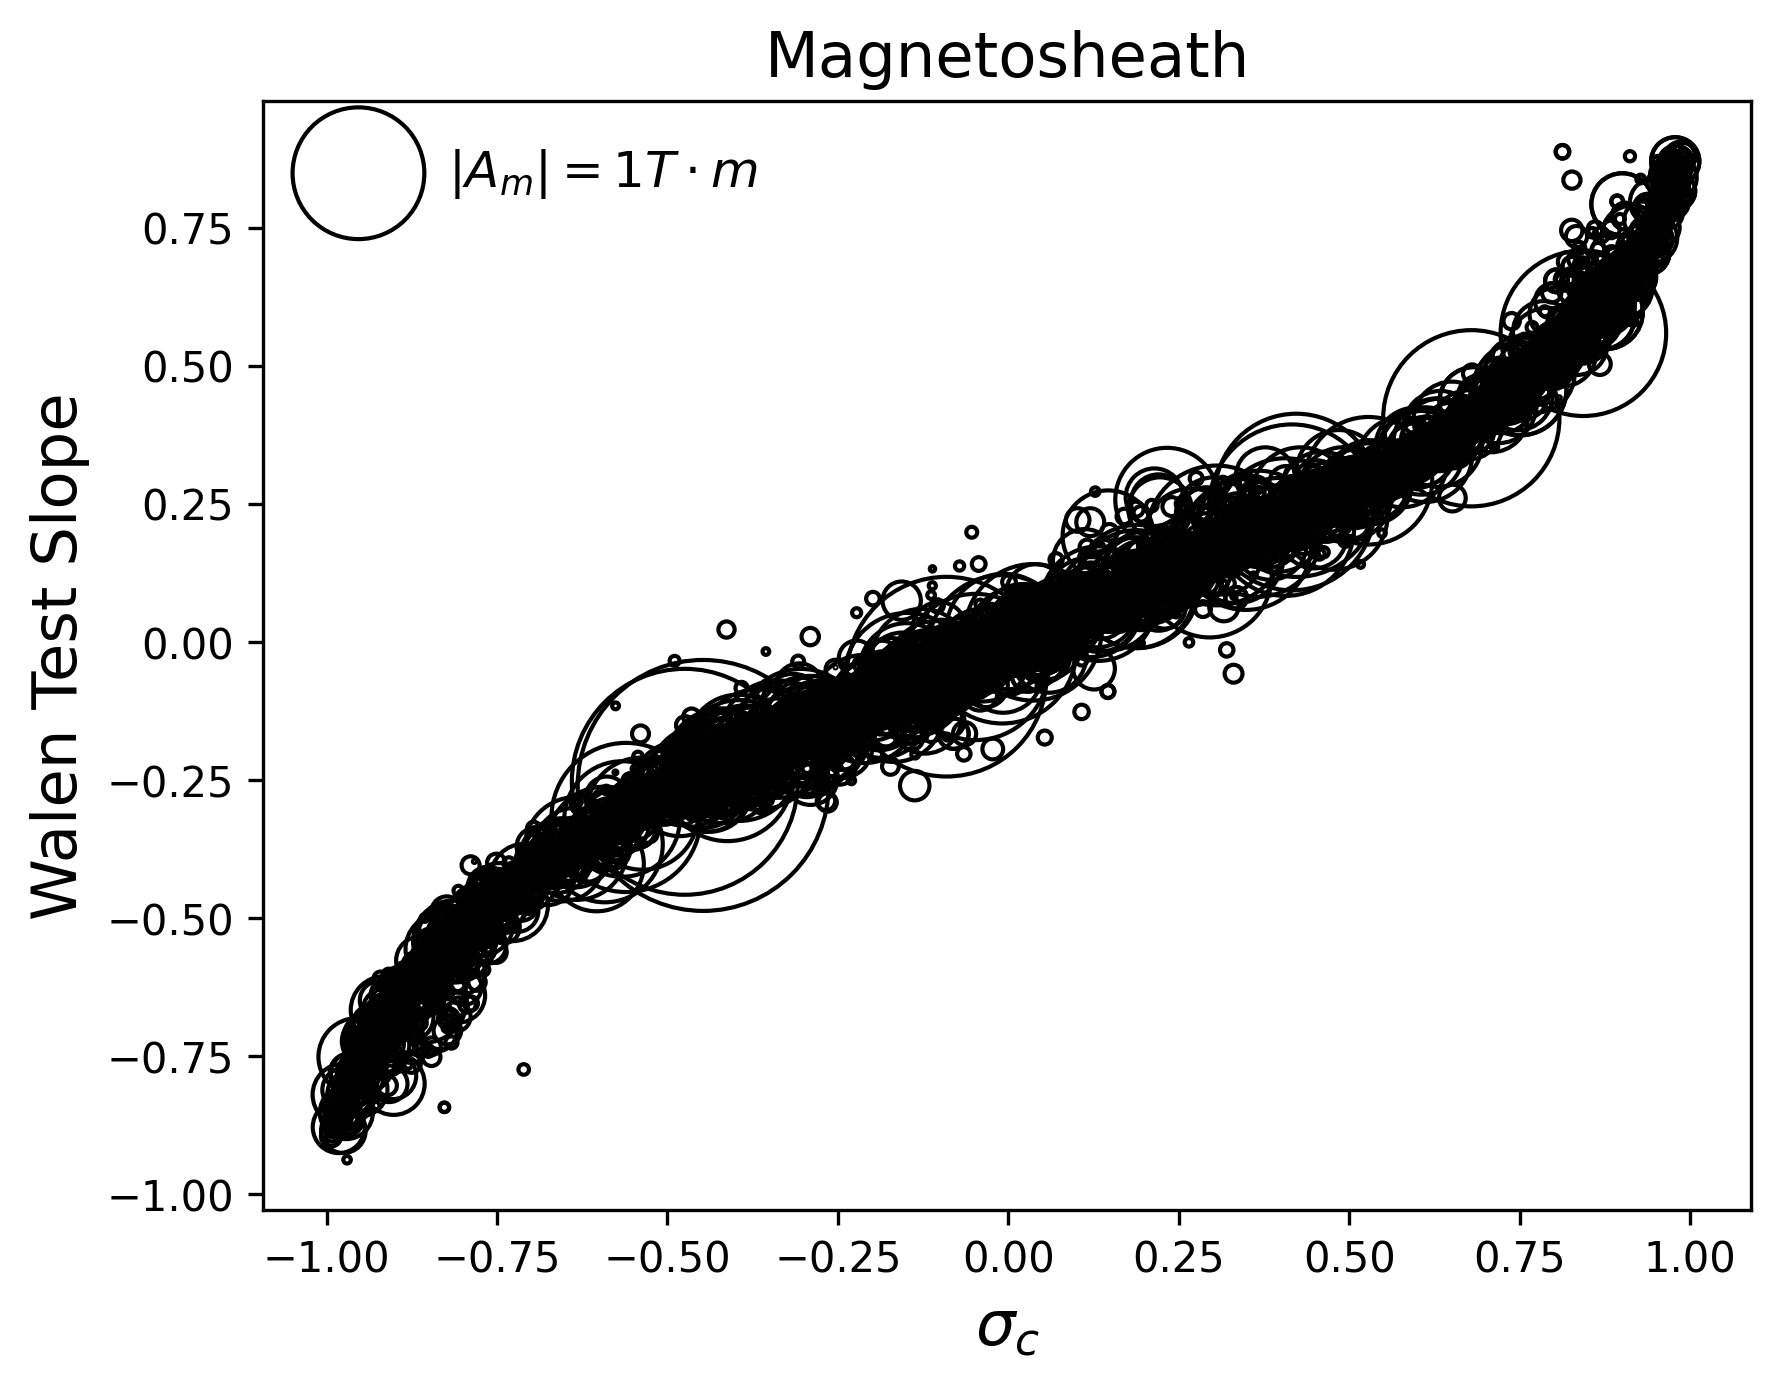
\includegraphics[width=0.7\textwidth]{Figures/GS analysis/walenTest_vs_crosshelicity_magnetosheath.png}
    \caption[Wal\'en test slope vs. reduced cross helicity]{Wal\'en test slope versus the reduced cross helicity for all of the events identified via GS analysis in both the solar wind (top) and magnetosheath (bottom). The size of the black circle represents the magnitude of the poloidal flux per unit length of each event. A reference circle of 1 Tm is present.}
    \label{fig:walen-crosshelicity}
\end{figure}

\section{Flow velocities and orientation of SFRs}
Lastly, a representation of the average flow velocities of the identified event intervals, \textit{i.e.}, $\mathbf{V_{HT}}$ vectors, is shown in Figure \ref{fig:VHT-xy}. For the identified SFR structures, I find that the corresponding flow velocities in the solar wind are fairly uniform and along the Sun-Earth direction; however, in the magnetosheath the flows appear to be largely deflected toward the dusk-side flank. Therefore the structures near the flanks (downstream of the quasi-perpendicular portion of the bow shock) ought to have elongated cross sections, resulting in large scale sizes. It is likely that while the structures may be compressed by the bow shock in the dimension along the normal direction of the bow shock, they may experience stretching along the dimension in the direction of the bulk flows, \textit{i.e.}, approximately perpendicular to the normal direction. This explains why some structures in the magnetosheath have large scale sizes, for instance, larger than the typical width of the magnetosheath itself.

\begin{figure}
    \centering
    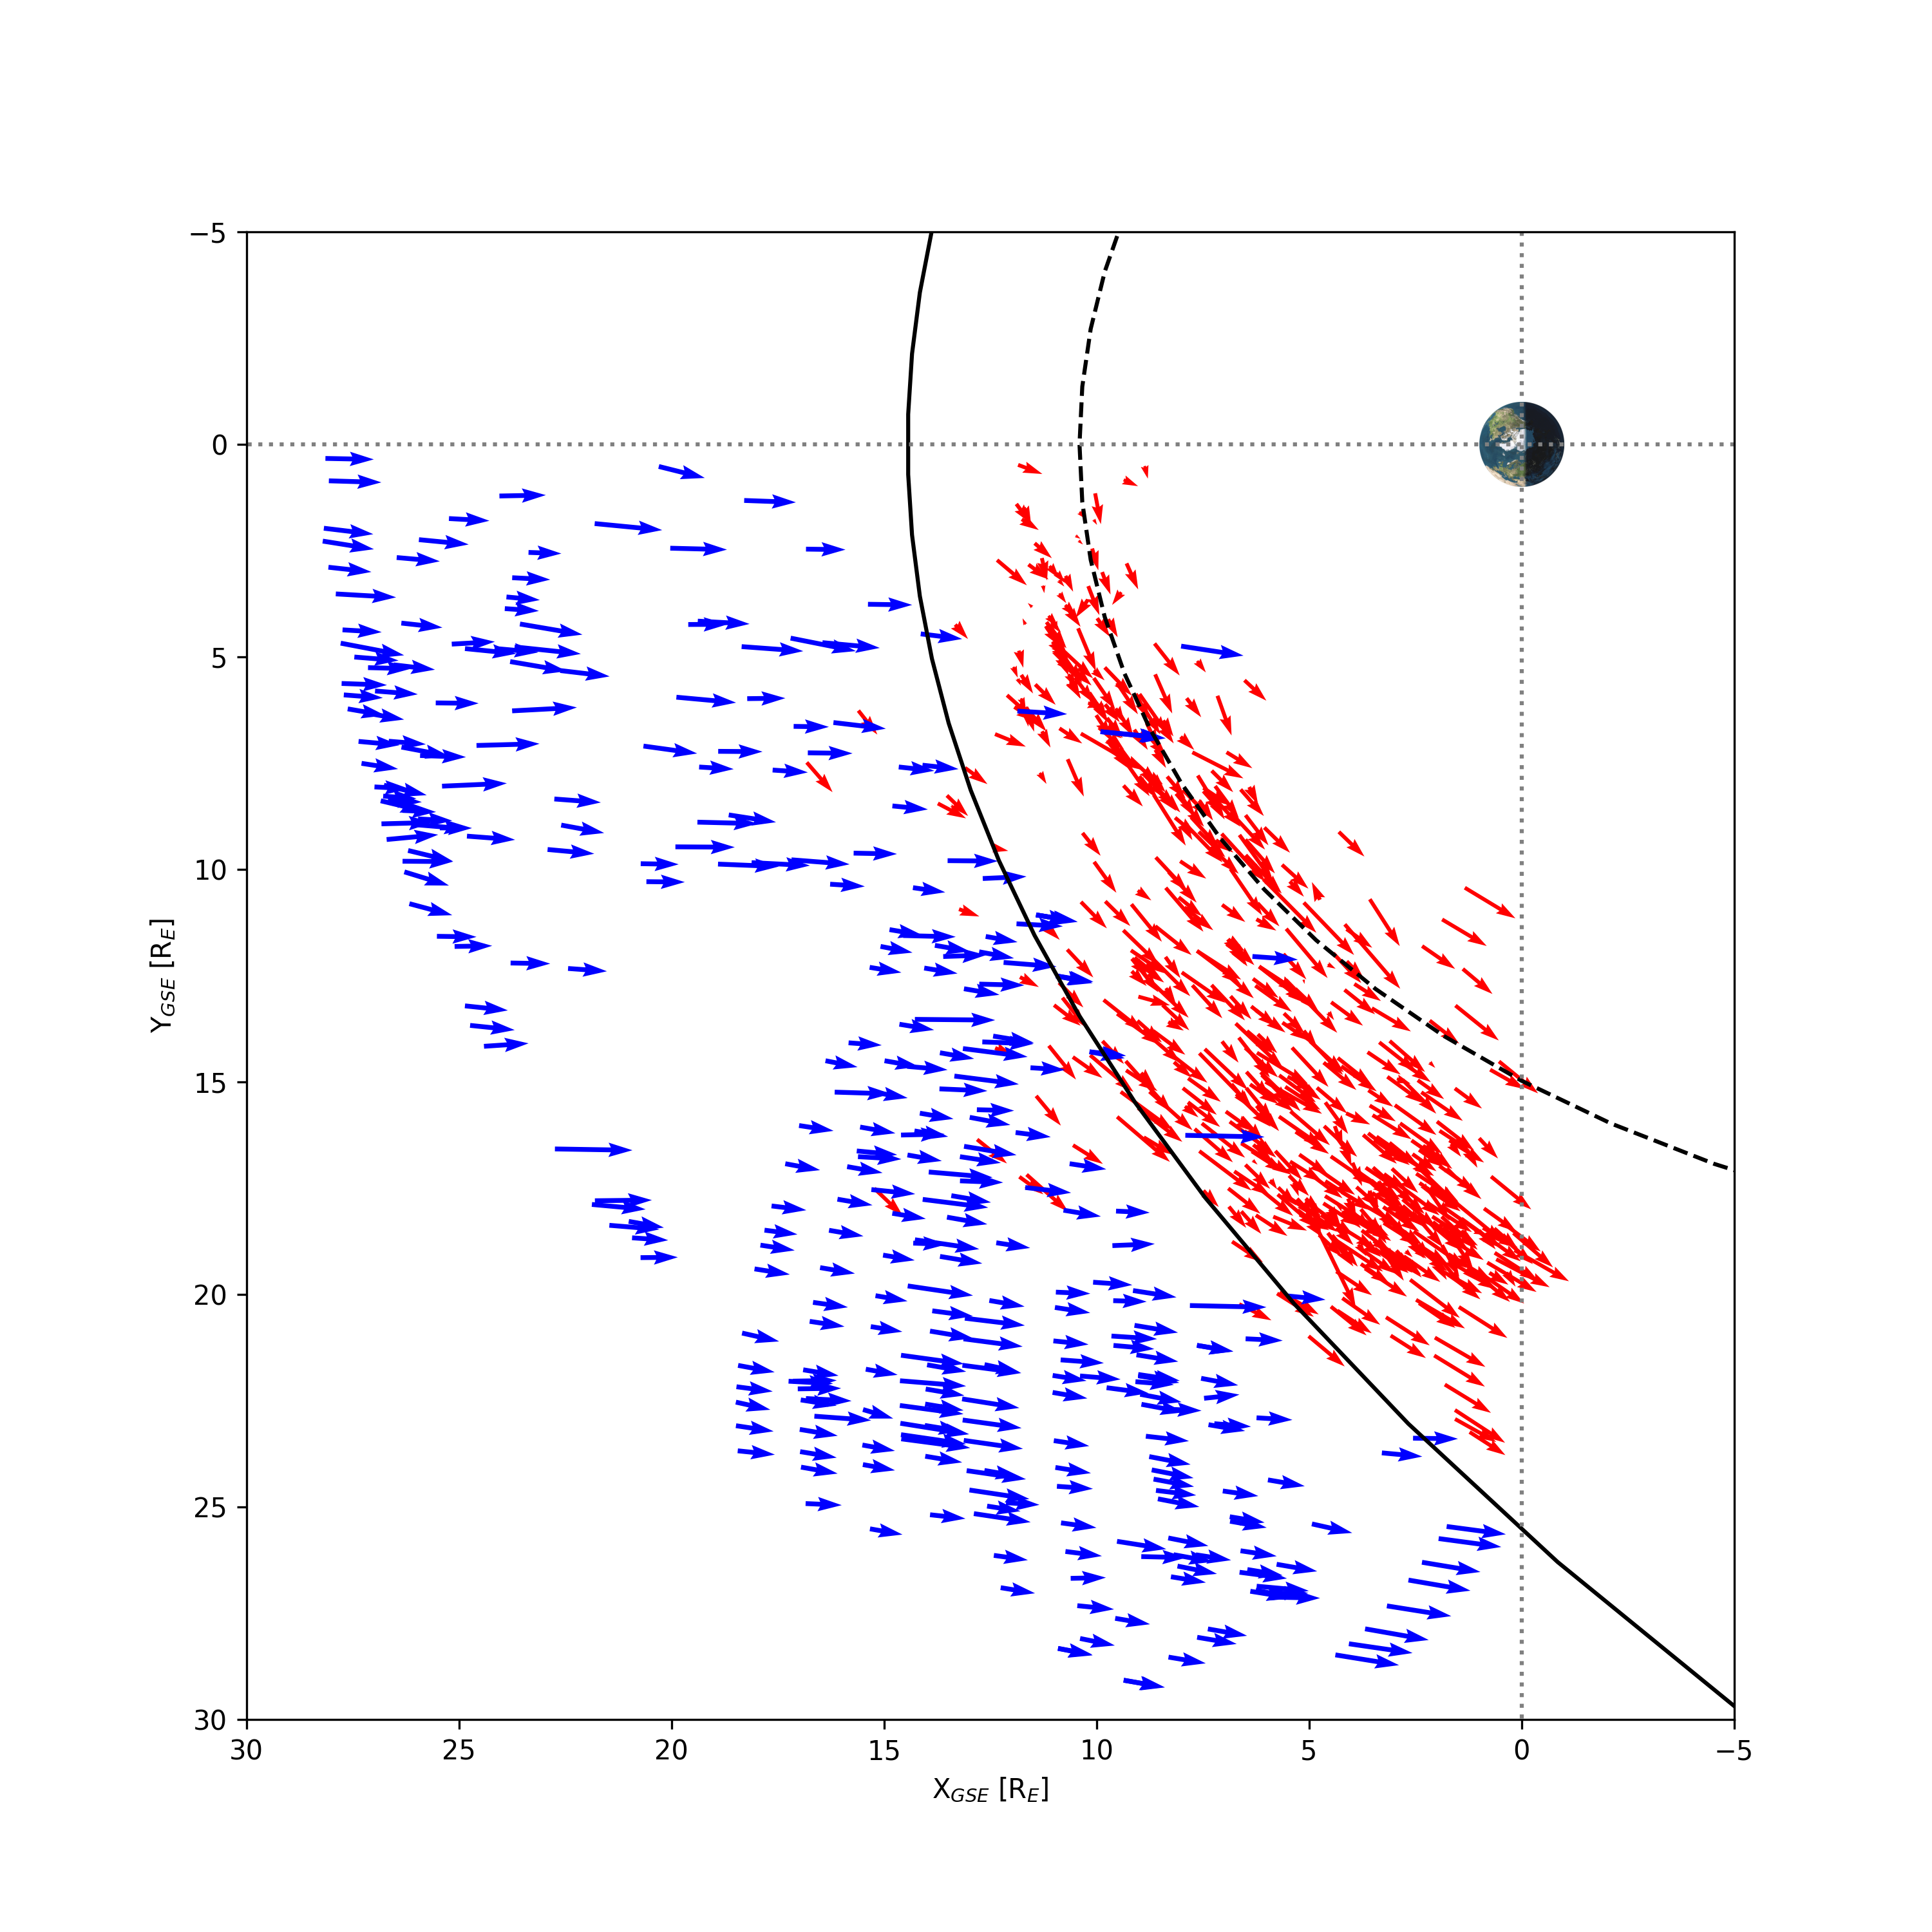
\includegraphics[width=\textwidth]{Figures/Orbits/VHT_xy.png}
    \caption[Orbit plot of flow vectors associated with the SFRs]{Plot showing the $\mathbf{V_{HT}}$ vectors at the locations of one-tenth of the total events identified in the solar wind (blue) and magnetosheath (red) on the GSE-$XY$ plane. The nominal bow shock (solid curve) and magnetopause (dashed curve) locations are drawn based on the models by \citet{Shue:1997} and \citet{SlavinHolzer:1984}, respectively. A reference vector of magnitude 400 km/s is shown in the upper left corner.}
    \label{fig:VHT-xy}
\end{figure}

% \begin{figure}
%     \centering
%     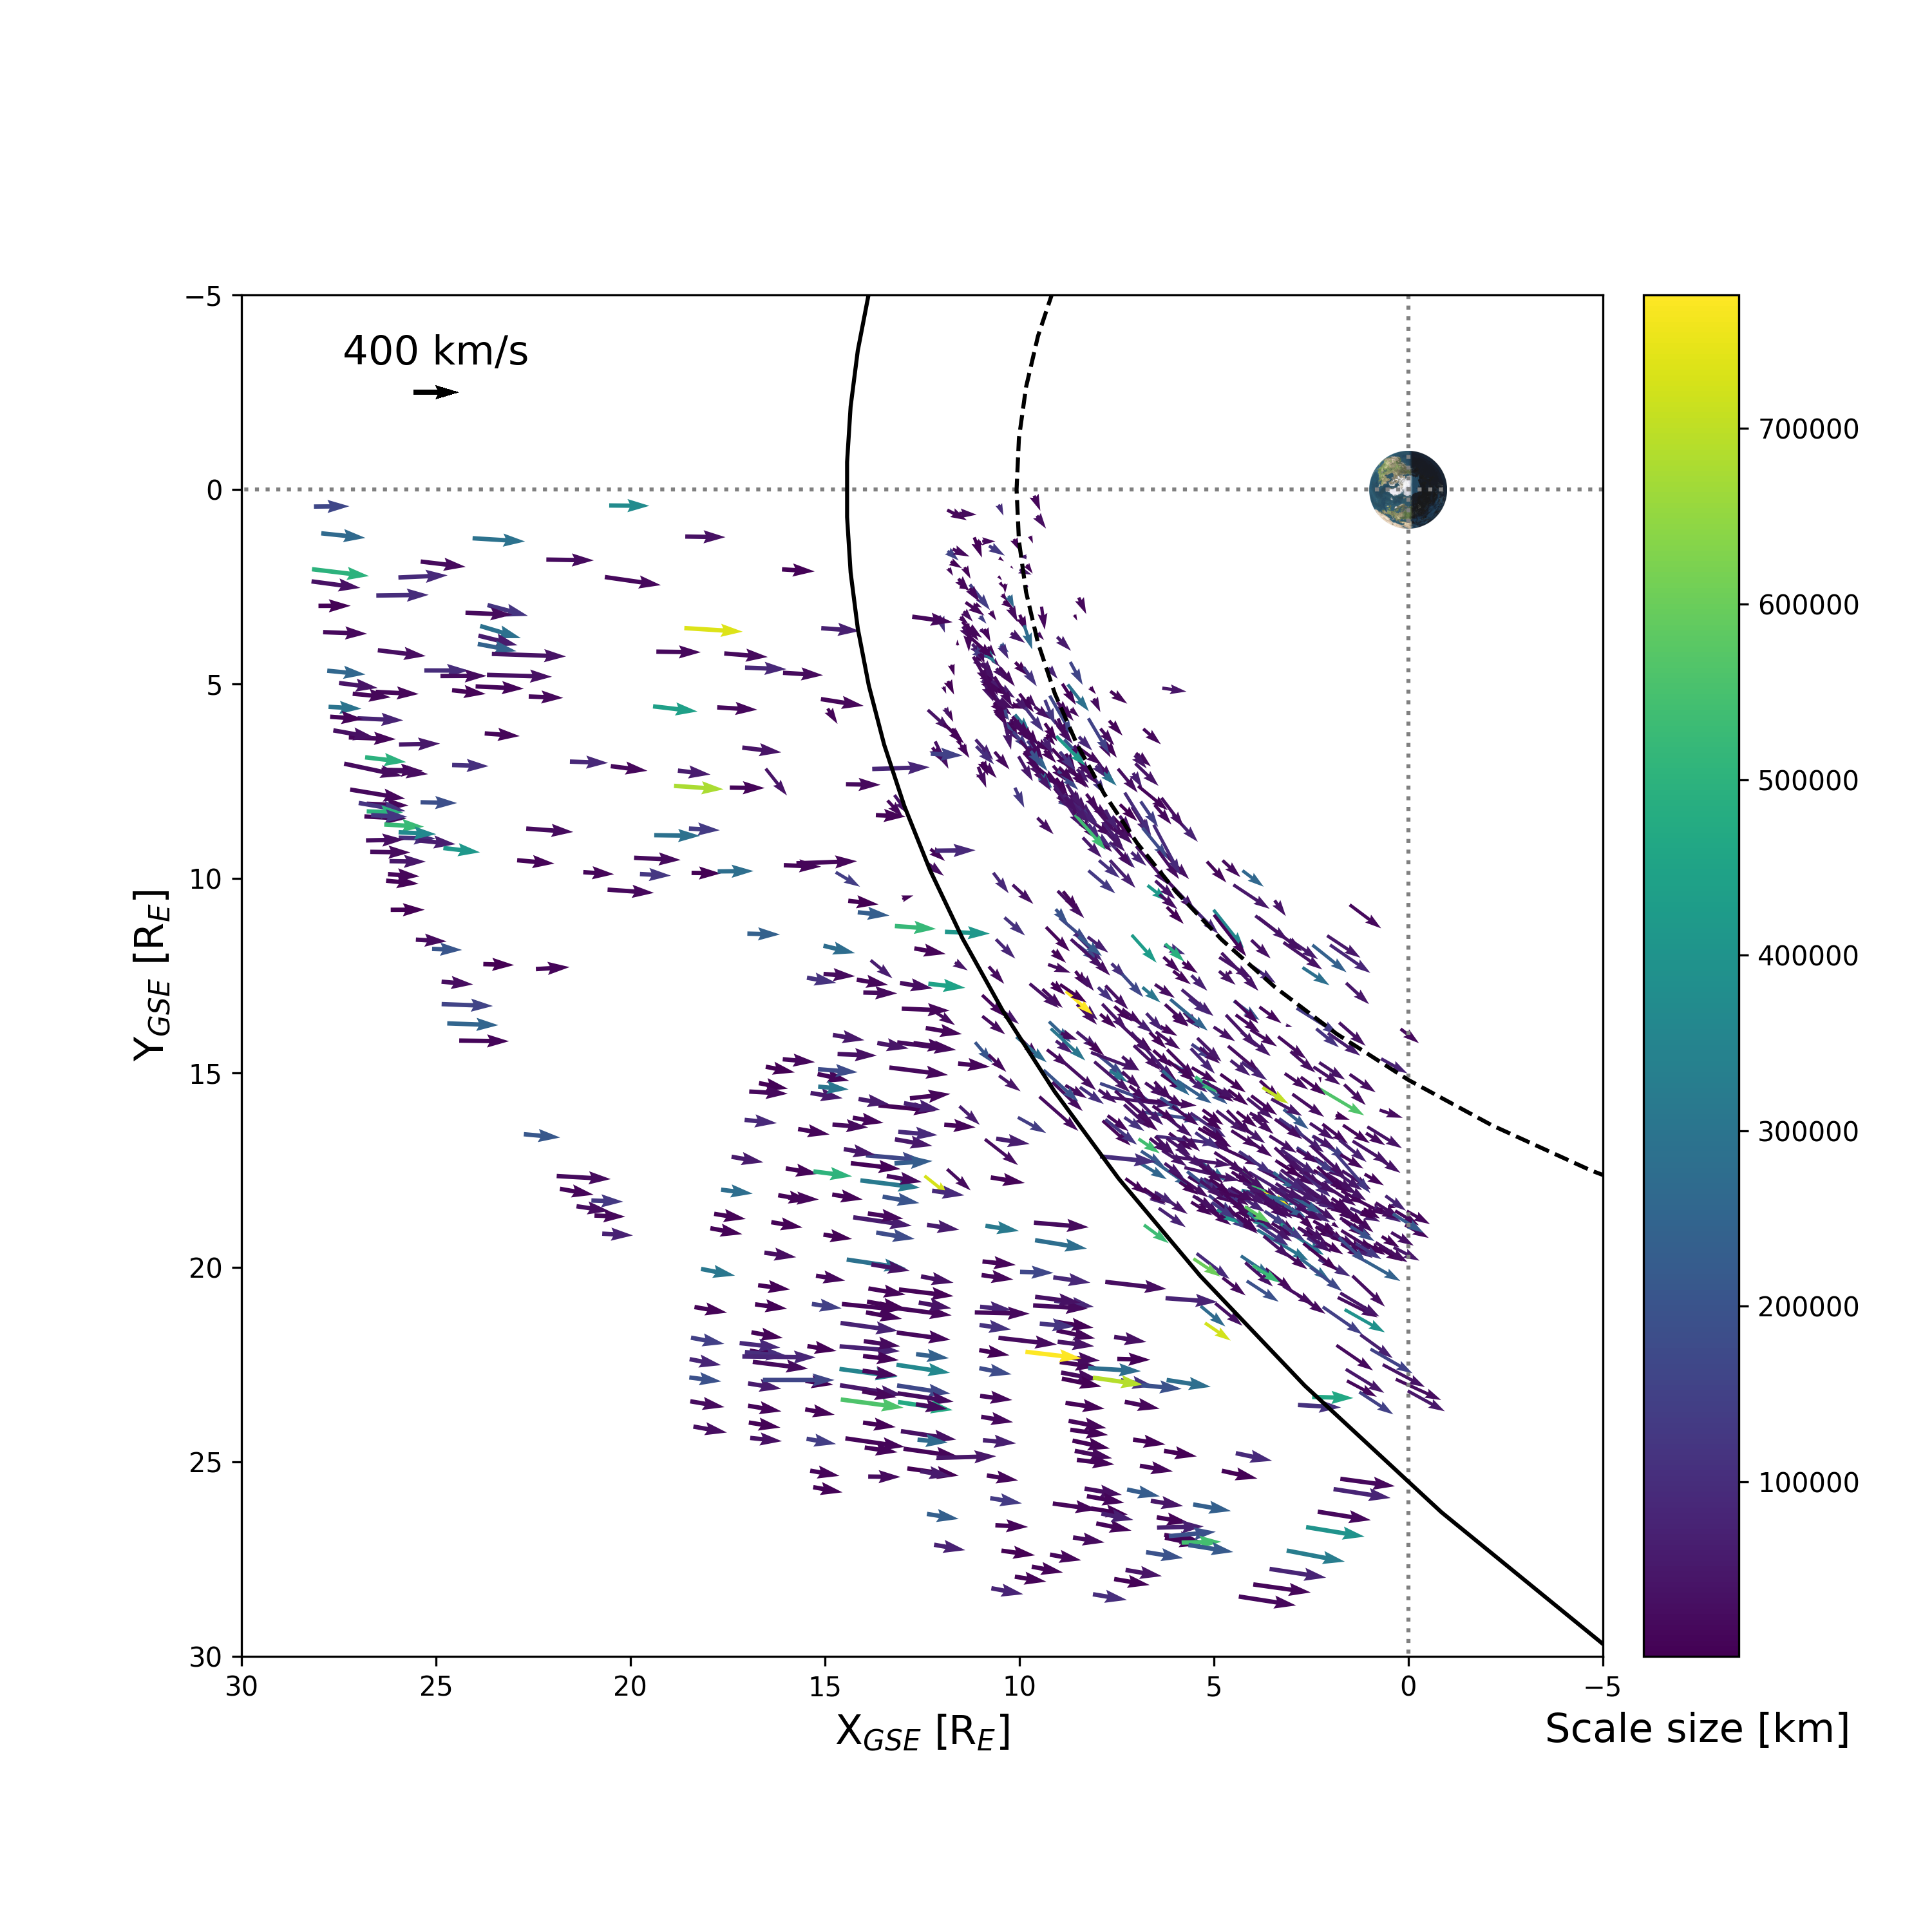
\includegraphics[width=\textwidth]{Figures/Orbits/VHT_xy_scalesize.png}
%     \caption[Orbit plot of flow vectors associated with the SFRs, in relation to their scale size]{Plot showing the $\mathbf{V_{HT}}$ vectors at the locations of one-tenth of the total events identified in the solar wind and magnetosheath on the GSE-$XY$ plane. The color gradient indicates the scale size of the SFRs associated with the $\mathbf{V_{HT}}$ vectors. The nominal bow shock (solid curve) and magnetopause (dashed curve) locations are drawn based on the models by \citet{Shue:1997} and \citet{SlavinHolzer:1984}, respectively. A reference vector of magnitude 400 km/s is shown in the upper left corner.}
%     \label{fig:VHT-scalesize}
% \end{figure}

Figure \ref{fig:histogram-orientation} shows the histograms of the $z$-axis orientation angles of the structures identified from the GS-based algorithm. For the solar wind, there is a single peak in the polar angle distribution centered around 60-70 degrees; however, for the magnetosheath there are two prominent peaks: one around 20-40 degrees and another from around 120-140 degrees. There is a significant trough in the distribution for the magnetosheath events around 80-100 degrees. The azimuthal angle has a flatter distribution in the solar wind than in the magnetosheath. The azimuthal angles in the solar wind show a small dip in the distribution around 170 degrees, and correspondingly there are two narrower peaks for the azimuthal angle in the magnetosheath, around 100 degrees and 260-300 degrees, possibly separated by 180 degrees. The shift in the dip between the two distributions is small, going from about 170 to 200 degrees for the two regions. Overall, the distributions of the azimuthal angle maintain similar shapes in the two regions, except for an additional enhanced peak near $\Phi\approx 0$ in the magnetosheath. The significant change in the polar angle in the magnetosheath indicates that the structures likely experience a rotation in the orientation downstream of the bow shock. It is possible that the interaction with the bow shock forces the change in the orientation of the magnetic structures.

\begin{figure}
    \centering
    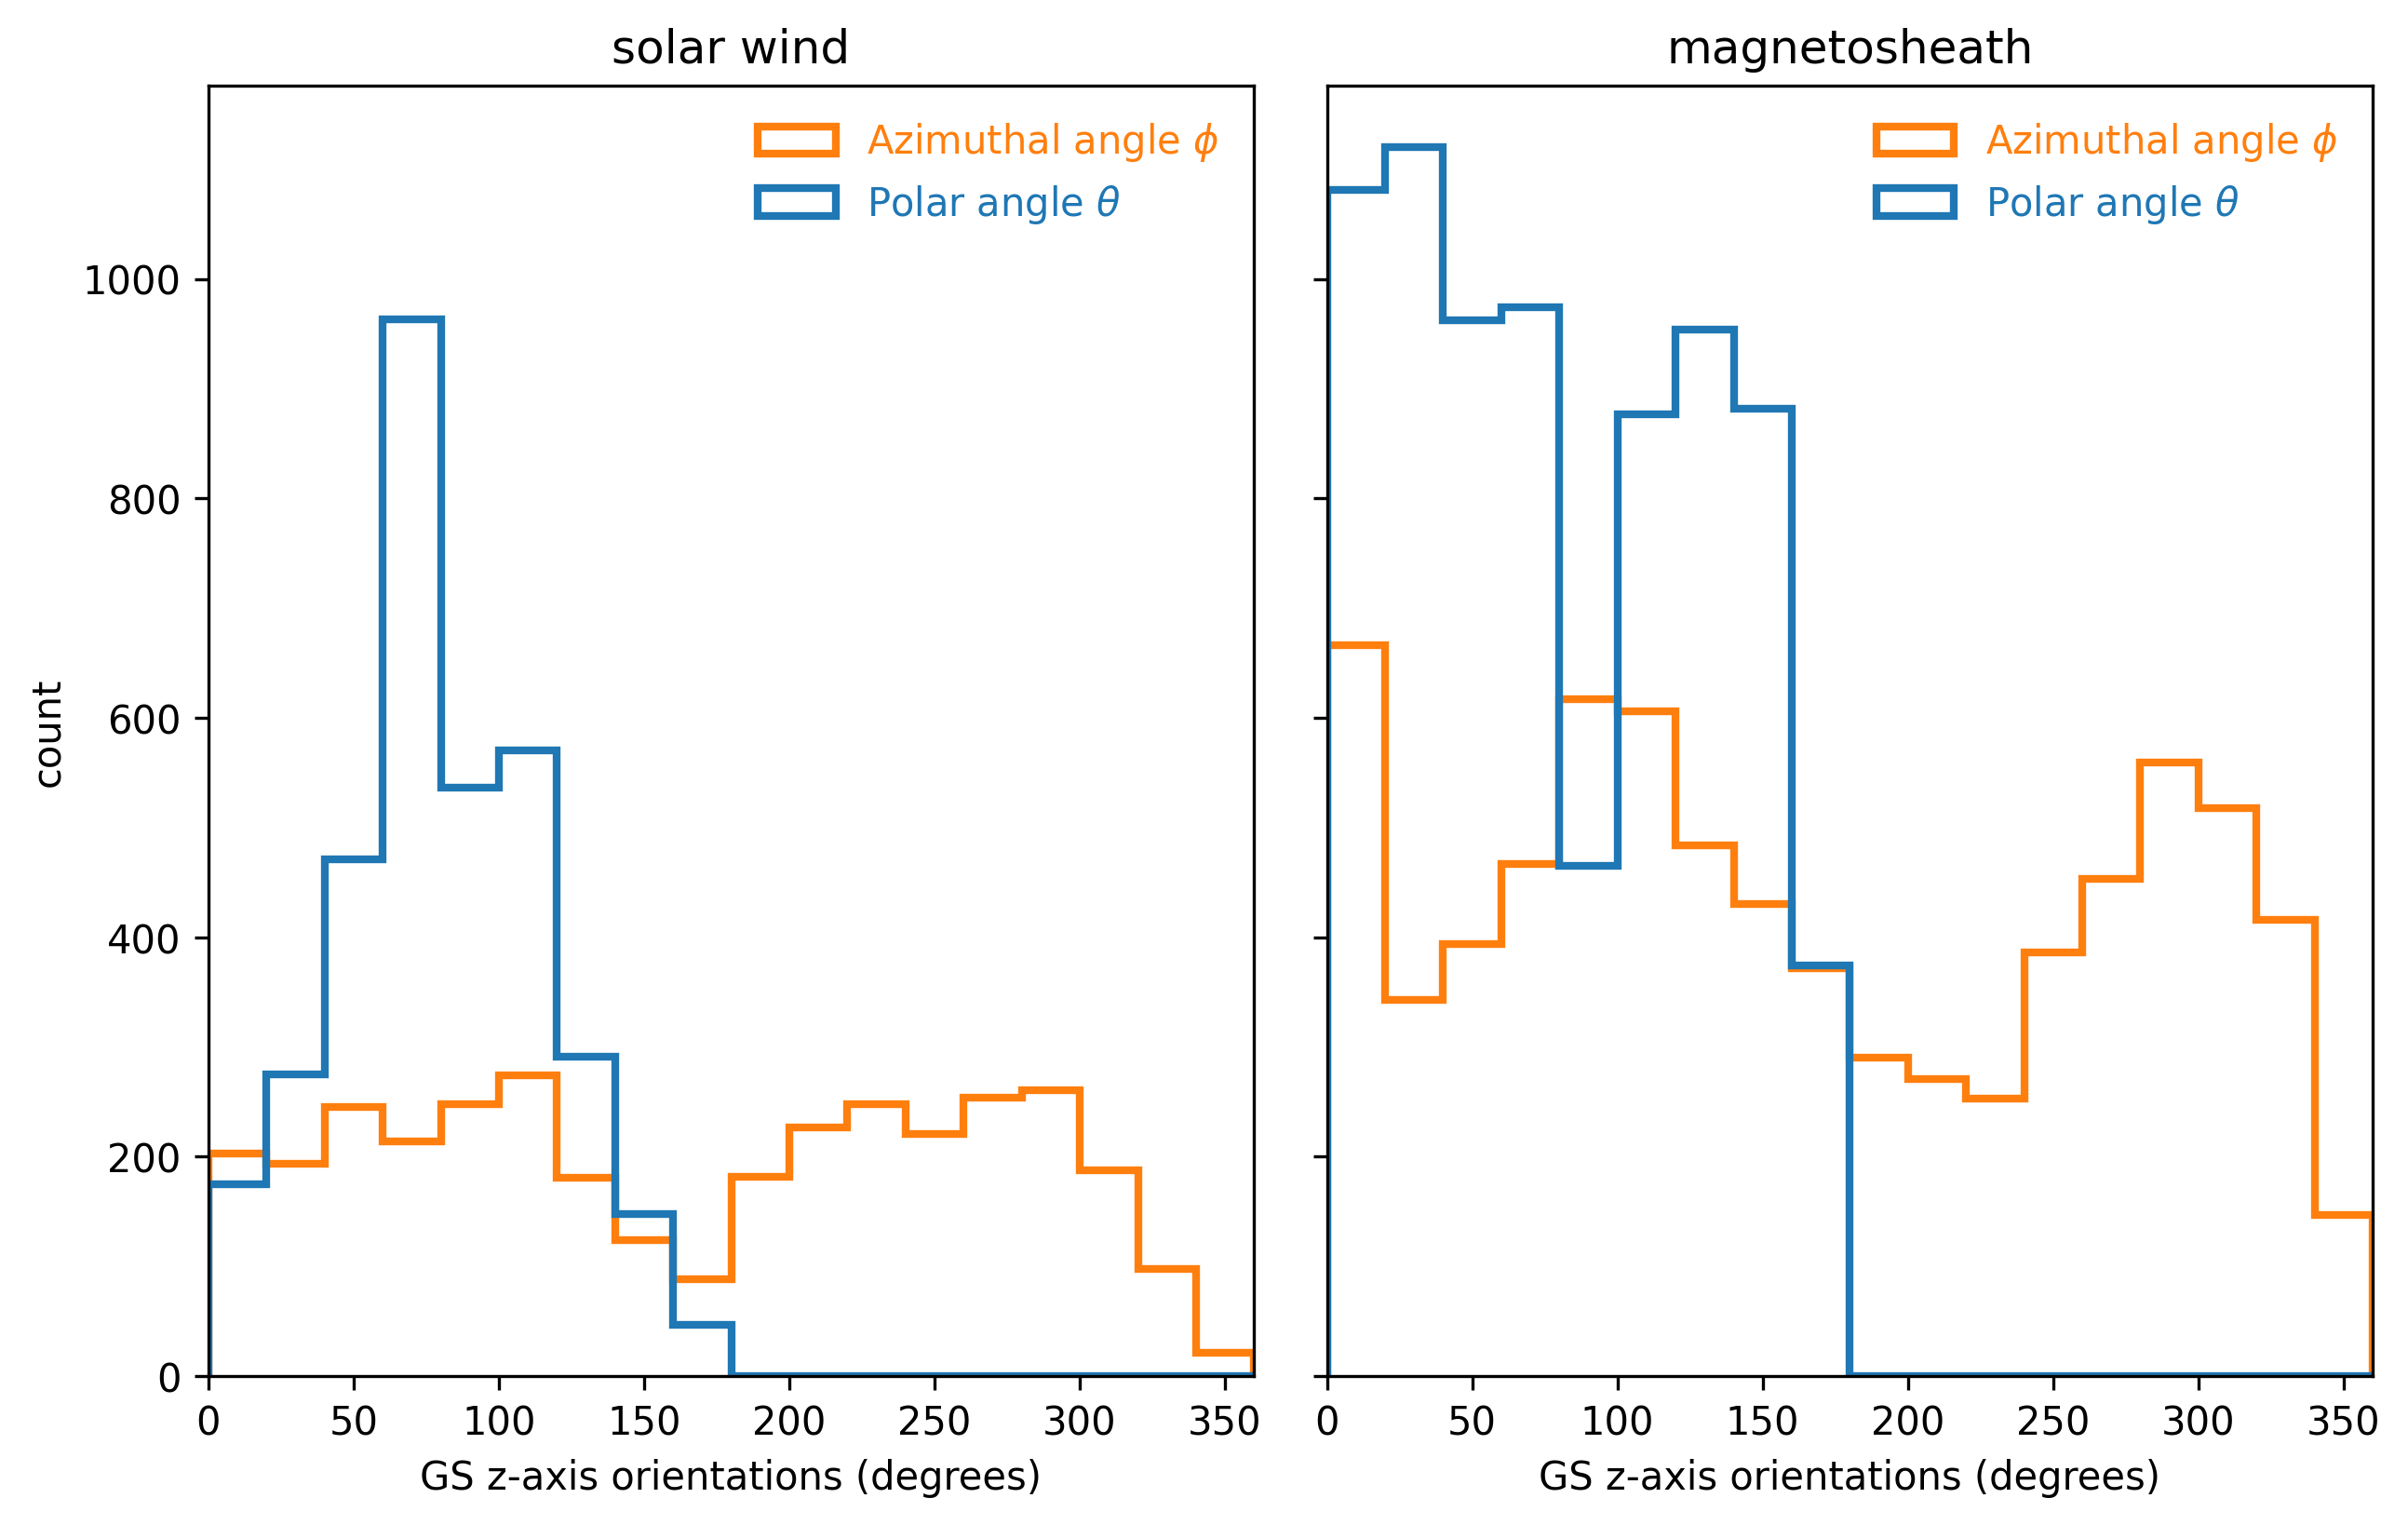
\includegraphics[width=\textwidth]{Figures/Histograms/histogram_orientation.png}
    \caption[Distributions of the azimuthal  and polar angles that define the $z$-axis of SFR structures]{Distributions of the azimuthal (orange) and polar angles (blue) of the directional angles that define the $z$-axis (in the GSE coordinate system) of the SFR structures identified from the GS-based analysis in the solar wind (left panel) and the magnetosheath (right panel).}
    \label{fig:histogram-orientation}
\end{figure}